\documentclass[final]{our-book}
\usepackage{makeidx}
% \usepackage{index}
\usepackage{our-multind}
\usepackage{enumerate}
\usepackage{times, mathptm}
\usepackage{sunil}
\usepackage{amsmath}
% \usepackage{times,amsmath}
\usepackage[thmmarks,amsmath]{ntheorem}
%\usepackage{multicol}
\usepackage{apalike}
\usepackage{xspace}

\usepackage{pifont}
\usepackage{float}
\floatstyle{ruled}
\restylefloat{figure}

\usepackage{array}
\usepackage{delarray}

\usepackage{fancybox}
%% the following two packages are needed to properly annotate exercises 
%% on both odd and even pages
\usepackage{mparhack}
\usepackage{chngpage}  

%%----------
%% HOL stuff
%%----------

% =====================================================================
%
% Macros for typesetting the HOL system manual
%
% =====================================================================

% ---------------------------------------------------------------------
% Abbreviations for words and phrases
% ---------------------------------------------------------------------

\newcommand\TUTORIAL{{\footnotesize\sl TUTORIAL}}
\newcommand\DESCRIPTION{{\footnotesize\sl DESCRIPTION}}
\newcommand\REFERENCE{{\footnotesize\sl REFERENCE}}
\newcommand\LOGIC{{\footnotesize\sl LOGIC}}
\newcommand\LIBRARIES{{\footnotesize\sl LIBRARIES}}

\newcommand{\bs}{\texttt{\char'134}} % backslash
\newcommand{\lb}{\texttt{\char'173}} % left brace
\newcommand{\rb}{\texttt{\char'175}} % right brace
\newcommand{\td}{\texttt{\char'176}} % tilde
\newcommand{\lt}{\texttt{\char'74}} % less than
\newcommand{\gt}{\texttt{\char'76}} % greater than
\newcommand{\dol}{\texttt{\char'44}} % dollar
% double back quotes ``
\newcommand{\dq}{\texttt{\char'140\char'140}}
%These macros were included by slind:

\newcommand{\holquote}[1]{\dq#1\dq}

\def\HOL{{\small HOL}}
\def\holn{\HOL}  % i.e. hol n(inety-eight), no digits in
                 % macro names is a bit of a pain; deciding to do away
                 % with hol98 nomenclature means that we just want to
                 % write HOL for hol98.
\def\holnversion{Kananaskis-7}
\def\holnsversion{Kananaskis~7} % version with space rather than hyphen
\def\LCF{{\small LCF}}
\def\LCFLSM{{\small LCF{\kern-.2em}{\normalsize\_}{\kern0.1em}LSM}}
\def\PPL{{\small PP}{\kern-.095em}$\lambda$}
\def\PPLAMBDA{{\small PPLAMBDA}}
\def\ML{{\small ML}}
\def\holmake{\texttt{Holmake}}

\newcommand\ie{\mbox{i{.}e{.}}}
\newcommand\eg{\mbox{e{.}g{.}}}
\newcommand\viz{\mbox{viz{.}}}
\newcommand\adhoc{\mbox{\it ad hoc}}
\newcommand\etal{{\it et al.\/}}
\newcommand\etc{\mbox{etc{.}}}

% ---------------------------------------------------------------------
% Simple abbreviations and macros for mathematical typesetting
% ---------------------------------------------------------------------

\newcommand\fun{{\to}}
\newcommand\prd{{\times}}

\newcommand\conj{\ \wedge\ }
\newcommand\disj{\ \vee\ }
\newcommand\imp{ \Rightarrow }
\newcommand\eqv{\ \equiv\ }
\newcommand\cond{\rightarrow}
\newcommand\vbar{\mid}
\newcommand\turn{\ \vdash\ }
\newcommand\hilbert{\varepsilon}
\newcommand\eqdef{\ \equiv\ }

\newcommand\natnums{\mbox{${\sf N}\!\!\!\!{\sf N}$}}
\newcommand\bools{\mbox{${\sf T}\!\!\!\!{\sf T}$}}

\newcommand\p{$\prime$}
\newcommand\f{$\forall$\ }
\newcommand\e{$\exists$\ }

\newcommand\orr{$\vee$\ }
\newcommand\negg{$\neg$\ }

\newcommand\arrr{$\rightarrow$}
\newcommand\hex{$\sharp $}

\newcommand{\uquant}[1]{\forall #1.\ }
\newcommand{\equant}[1]{\exists #1.\ }
\newcommand{\hquant}[1]{\hilbert #1.\ }
\newcommand{\iquant}[1]{\exists ! #1.\ }
\newcommand{\lquant}[1]{\lambda #1.\ }

\newcommand{\leave}[1]{\\[#1]\noindent}
\newcommand\entails{\mbox{\rule{.3mm}{4mm}\rule[2mm]{.2in}{.3mm}}}

% ---------------------------------------------------------------------
% Font-changing commands
% ---------------------------------------------------------------------

\newcommand{\theory}[1]{\hbox{{\small\tt #1}}}
\newcommand{\theoryimp}[1]{\texttt{#1}}

\newcommand{\con}[1]{{\sf #1}}
\newcommand{\rul}[1]{{\tt #1}}
\newcommand{\ty}[1]{\textsl{#1}}

\newcommand{\ml}[1]{\mbox{{\def\_{\char'137}\texttt{#1}}}}
\newcommand{\holtxt}[1]{\ml{#1}}
\newcommand\ms{\tt}
\newcommand{\s}[1]{{\small #1}}

\newcommand{\pin}[1]{{\bf #1}}
\def\m#1{\mbox{\normalsize$#1$}}

% ---------------------------------------------------------------------
% Abbreviations for particular mathematical constants etc.
% ---------------------------------------------------------------------

\newcommand\T{\con{T}}
\newcommand\F{\con{F}}
\newcommand\OneOne{\con{One\_One}}
\newcommand\OntoSubset{\con{Onto\_Subset}}
\newcommand\Onto{\con{Onto}}
\newcommand\TyDef{\con{Type\_Definition}}
\newcommand\Inv{\con{Inv}}
\newcommand\com{\con{o}}
\newcommand\Id{\con{I}}
\newcommand\MkPair{\con{Mk\_Pair}}
\newcommand\IsPair{\con{Is\_Pair}}
\newcommand\Fst{\con{Fst}}
\newcommand\Snd{\con{Snd}}
\newcommand\Suc{\con{Suc}}
\newcommand\Nil{\con{Nil}}
\newcommand\Cons{\con{Cons}}
\newcommand\Hd{\con{Hd}}
\newcommand\Tl{\con{Tl}}
\newcommand\Null{\con{Null}}
\newcommand\ListPrimRec{\con{List\_Prim\_Rec}}


\newcommand\SimpRec{\con{Simp\_Rec}}
\newcommand\SimpRecRel{\con{Simp\_Rec\_Rel}}
\newcommand\SimpRecFun{\con{Simp\_Rec\_Fun}}
\newcommand\PrimRec{\con{Prim\_Rec}}
\newcommand\PrimRecRel{\con{Prim\_Rec\_Rel}}
\newcommand\PrimRecFun{\con{Prim\_Rec\_Fun}}

\newcommand\bool{\ty{bool}}
\newcommand\num{\ty{num}}
\newcommand\ind{\ty{ind}}
\newcommand\lst{\ty{list}}

% ---------------------------------------------------------------------
% \minipagewidth = \textwidth minus 1.02 em
% ---------------------------------------------------------------------

\newlength{\minipagewidth}
\setlength{\minipagewidth}{\textwidth}
\addtolength{\minipagewidth}{-1.02em}

% ---------------------------------------------------------------------
% Environment for the items on the title page of a case study
% ---------------------------------------------------------------------

\newenvironment{inset}[1]{\noindent{\large\bf #1}\begin{list}%
{}{\setlength{\leftmargin}{\parindent}%
\setlength{\topsep}{-.1in}}\item }{\end{list}\vskip .4in}

% ---------------------------------------------------------------------
% Macros for little HOL sessions displayed in boxes.
%
% Usage: (1) \setcounter{sessioncount}{1} resets the session counter
%
%        (2) \begin{session}\begin{verbatim}
%             .
%              < lines from hol session >
%             .
%            \end{verbatim}\end{session}
%
%            typesets the session in a numbered box.
% ---------------------------------------------------------------------

\newlength{\hsbw}
\setlength{\hsbw}{\textwidth}
\addtolength{\hsbw}{-\arrayrulewidth}
\addtolength{\hsbw}{-\tabcolsep}
\newcommand\HOLSpacing{13pt}

\newcounter{sessioncount}
\setcounter{sessioncount}{0}

\newenvironment{session}{\begin{flushleft}
 \refstepcounter{sessioncount}
 \begin{tabular}{@{}|c@{}|@{}}\hline
 \begin{minipage}[b]{\hsbw}
 \vspace*{-.5pt}
 \begin{flushright}
 \rule{0.01in}{.15in}\rule{0.3in}{0.01in}\hspace{-0.35in}
 \raisebox{0.04in}{\makebox[0.3in][c]{\footnotesize\sl \thesessioncount}}
 \end{flushright}
 \vspace*{-.55in}
 \begingroup\small\baselineskip\HOLSpacing}{\endgroup\end{minipage}\\ \hline
 \end{tabular}
 \end{flushleft}}

% ---------------------------------------------------------------------
% Macro for boxed ML functions, etc.
%
% Usage: (1) \begin{holboxed}\begin{verbatim}
%               .
%               < lines giving names and types of mk functions >
%               .
%            \end{verbatim}\end{holboxed}
%
%            typesets the given lines in a box.
%
%            Conventions: lines are left-aligned under the "g" of begin,
%            and used to highlight primary reference for the ml function(s)
%            that appear in the box.
% ---------------------------------------------------------------------

\newenvironment{holboxed}{\begin{flushleft}
  \begin{tabular}{@{}|c@{}|@{}}\hline
  \begin{minipage}[b]{\hsbw}
% \vspace*{-.55in}
  \vspace*{.06in}
  \begingroup\small\baselineskip\HOLSpacing}{\endgroup\end{minipage}\\ \hline
  \end{tabular}
  \end{flushleft}}

% ---------------------------------------------------------------------
% Macro for unboxed ML functions, etc.
%
% Usage: (1) \begin{hol}\begin{verbatim}
%               .
%               < lines giving names and types of mk functions >
%               .
%            \end{verbatim}\end{hol}
%
%            typesets the given lines exactly like {boxed}, except there's
%            no box.
%
%            Conventions: lines are left-aligned under the "g" of begin,
%            and used to display ML code in verbatim, left aligned.
% ---------------------------------------------------------------------

\newenvironment{hol}{\begin{flushleft}
 \begin{tabular}{c@{}@{}}
 \begin{minipage}[b]{\hsbw}
% \vspace*{-.55in}
 \vspace*{.06in}
 \begingroup\small\baselineskip\HOLSpacing}{\endgroup\end{minipage}\\
 \end{tabular}
 \end{flushleft}}

% ---------------------------------------------------------------------
% Emphatic brackets
% ---------------------------------------------------------------------

\newcommand\leb{\lbrack\!\lbrack}
\newcommand\reb{\rbrack\!\rbrack}


% ---------------------------------------------------------------------
% Quotations
% ---------------------------------------------------------------------


%These macros were included by ap; they are used in Chapters 9 and 10
%of the HOL DESCRIPTION

\newcommand{\inds}%standard infinite set
 {\mbox{\rm I}}

\newcommand{\ch}%standard choice function
 {\mbox{\rm ch}}

\newcommand{\den}[1]%denotational brackets
 {[\![#1]\!]}

\newcommand{\two}%standard 2-element set
 {\mbox{\rm 2}}

%macros for pictures in latex

\def\puthrule(#1,#2)#3{\put(#1,#2){\line(1,0){#3}}}
\def\putvrule(#1,#2)#3{\put(#1,#2){\line(0,1){#3}}}
\def\putdot(#1){\put(#1){\circle*{0.2}}}
\def\ignore#1{}
\def\putgrid(#1,#2)(#3,#4){\multiput(#1,#2)(1,0){#3}{\circle*{0.2}}
\multiput(#1,#2)(0,1){#4}{\circle*{0.2}}}

\def\putdevice(#1,#2)#3{\put(#1,#2){\framebox(4,2){\small{\tt #3}}}}
\def\putport(#1,#2)#3{\put(#1,#2){\makebox(4,1){\small{\tt #3}}}}


% =====================================================================
% Macros for typesetting hol reference manual entries
% =====================================================================

% ---------------------------------------------------------------------
% boolean flag for verbose printing of reference manual typesetting
% ---------------------------------------------------------------------

\newif\ifverboseref
\verbosereffalse                          % don't be verbose

% ---------------------------------------------------------------------
% Macro for generating right-hand page running titles.
% ---------------------------------------------------------------------

\makeatletter

\def\mkhead{\futurelet\@t\chsize}
\def\chsize#1.{\ifx a\@t \markright{{\protect\bf #1}}\else
               \ifx b\@t \markright{{\protect\bf #1}}\else
               \ifx c\@t \markright{{\protect\bf #1}}\else
               \ifx d\@t \markright{{\protect\bf #1}}\else
               \ifx e\@t \markright{{\protect\bf #1}}\else
               \ifx f\@t \markright{{\protect\bf #1}}\else
               \ifx g\@t \markright{{\protect\bf #1}}\else
               \ifx h\@t \markright{{\protect\bf #1}}\else
               \ifx i\@t \markright{{\protect\bf #1}}\else
               \ifx j\@t \markright{{\protect\bf #1}}\else
               \ifx k\@t \markright{{\protect\bf #1}}\else
               \ifx l\@t \markright{{\protect\bf #1}}\else
               \ifx m\@t \markright{{\protect\bf #1}}\else
               \ifx n\@t \markright{{\protect\bf #1}}\else
               \ifx o\@t \markright{{\protect\bf #1}}\else
               \ifx p\@t \markright{{\protect\bf #1}}\else
               \ifx q\@t \markright{{\protect\bf #1}}\else
               \ifx r\@t \markright{{\protect\bf #1}}\else
               \ifx s\@t \markright{{\protect\bf #1}}\else
               \ifx t\@t \markright{{\protect\bf #1}}\else
               \ifx u\@t \markright{{\protect\bf #1}}\else
               \ifx v\@t \markright{{\protect\bf #1}}\else
               \ifx w\@t \markright{{\protect\bf #1}}\else
               \ifx z\@t \markright{{\protect\bf #1}}\else
               \ifx y\@t \markright{{\protect\bf #1}}\else
               \ifx z\@t \markright{{\protect\bf #1}}\else
               \markright{{\protect\small\bf #1}}\fi
               \fi\fi\fi\fi\fi\fi\fi\fi\fi\fi\fi\fi\fi\fi\fi
               \fi\fi\fi\fi\fi\fi\fi\fi\fi\fi}

\makeatother

% ---------------------------------------------------------------------
% \DOC{<object>}  : start a manual entry for <object>.
% ---------------------------------------------------------------------

\newcommand{\DOC}[2]%
{\bigskip
 {\ifverboseref{\def\_{\string_}\typeout{Typesetting: #1}}\fi}
 \bgroup\samepage               % ended after \TYPE
 \mkhead #1.
 \begin{flushleft}
 \begin{tabular}{|c|}\hline
 \begin{minipage}{\minipagewidth}
 \bigskip
 {\def\_{\char'137}\LARGE\tt #2}\autoindex{#1@{\tt #1}}
 \bigskip
 \end{minipage}\\ \hline
 \end{tabular}
 \end{flushleft}
 \vskip10pt}

% ---------------------------------------------------------------------
% \setseps = set the spacing parameters for above and below displays
% ---------------------------------------------------------------------
\def\setseps{\partopsep=0mm\topsep=12pt plus2pt minus2pt}

% ---------------------------------------------------------------------
% flag for typesetting SEEALSO list
% ---------------------------------------------------------------------
\newif\ifseealso
\seealsofalse                     % start false.

% ---------------------------------------------------------------------
% \TYPE {<thing>} : {<type>}
% ---------------------------------------------------------------------
\def\TYPE{\noindent}

% ---------------------------------------------------------------------
% Commands for parts of a \DOC:
%    \SYNOPSIS
%    \DESCRIBE
%    \FAILURE
%    \EXAMPLE
%    \USES
%    \SEEALSO
% ---------------------------------------------------------------------

\newcommand\beforeskip{\vspace{12pt plus4pt minus4pt}}

\newcommand{\SYNOPSIS}%
{\beforeskip\leftline{\large\bf Synopsis}\nobreak\noindent}

\newcommand{\DESCRIBE}%
{\beforeskip\leftline{\large\bf Description}\nobreak\noindent}

\newcommand{\FAILURE}%
{\beforeskip\leftline{\large\bf Failure}\nobreak\noindent}

\newcommand{\EXAMPLE}%
{\beforeskip\leftline{\large\bf Example}\nobreak\noindent}

\newcommand{\USES}%
{\beforeskip\leftline{\large\bf Uses}\nobreak\noindent}

\newcommand{\COMMENTS}%
{\beforeskip\leftline{\large\bf Comments}\nobreak\noindent}

\newcommand{\SEEALSO}%
{\beforeskip\seealsotrue\leftline{\large\bf See also}\nobreak\noindent%
\bgroup\raggedright\small\tt\catcode`\_=12}

% ---- added by S-K Chin --------
\newcommand{\IMPLEMENTATION}%
{\beforeskip\leftline{\large\bf Implementation}\nobreak\noindent}


% ---------------------------------------------------------------------
% \ENDDOC = do nothing, but close off the group started by \SEEALSO
% ---------------------------------------------------------------------

\newcommand{\ENDDOC}{\ifseealso \egroup\seealsofalse \else \relax \fi}

% =====================================================================
% Commands for typesetting theorems
% =====================================================================

\makeatletter

% ---------------------------------------------------------------------
% define \@xboxverb<thing>\ENDTHEOREM to mean <thing>\ENDTHEOREM
% ---------------------------------------------------------------------

\begingroup \catcode `|=0 \catcode `[= 1
\catcode`]=2 \catcode `\{=12 \catcode `\}=12
\catcode`\\=12 |gdef|@xboxverb#1\ENDTHEOREM[#1|ENDTHEOREM]
|endgroup

% ---------------------------------------------------------------------
% \bboxverb<thing> = <thing> in a verbatim box 5mm from left margin
% ---------------------------------------------------------------------

\def\@boxverb{\bgroup\leftskip=5mm\parindent\z@
\parfillskip=\@flushglue\parskip\z@
\obeylines\small\tt \catcode``=13 \@noligs \let\do\@makeother \dospecials}

\def\boxverb{\@boxverb \frenchspacing\@vobeyspaces \@xboxverb}

% ---------------------------------------------------------------------
% \ENDTHEOREM just finishes off the group (and kick page if necessary)
% ---------------------------------------------------------------------

\def\ENDTHEOREM{\egroup\filbreak}

% ---------------------------------------------------------------------
% \THEOREM <name> <thy> ... \ENDTHEOREM = typeset a theorem
% ---------------------------------------------------------------------

\def\THEOREM #1 #2 {
 \autoindex{#1@{\tt #1}}
   \vspace{4mm plus2mm minus1mm}
\noindent {\def\_{{\char'137}}\small\tt #1}\quad({\small\tt #2}) \par \boxverb
}

\makeatother

% ---------------------------------------------------------------------
% The theory name \none = italic "none"
% ---------------------------------------------------------------------

\def\none{{\it none}}

\usepackage{proof}
\usepackage{holtex}
\usepackage{holtexbasic}

%\includeonly{introduction}
%\includeonly{networkedAC}
%\includeonly{coreRules,basicACconcepts}


%% Added 5 Nov 2004
%%
%% The following code will enable both LaTeX (and dvips) and PDF LaTeX
%% to work on the same files, making both our lives much happier.
%%
\ifx\pdfoutput\undefined
\usepackage[dvips]{graphicx}
\else
\usepackage[pdftex]{graphicx}
\usepackage{epstopdf}
\pdfcompresslevel=9
\fi
% if using pdflatex, we must use our .pdf images instead of .(e?)ps
\ifx\pdfoutput\undefined
\else
\DeclareGraphicsExtensions{.pdf,.gif,.jpg} % the formats we have images in
\fi

%\usepackage[dvipsnames,usenames]{color}
\usepackage[svgnames]{xcolor}

%\usepackage{fancyheadings}
\usepackage{amssymb, amsmath}

% \usepackage{float}
% %\floatstyle{ruled}
% \floatstyle{boxed}
% \restylefloat{figure}
% \restylefloat{table}


% %\usepackage{theorem}

%% get parts to show up correctly in the table of contents
\makeatletter

\let\toc@draw\relax
\def\l@part#1#2{%
 \toc@draw
 \gdef\toc@draw{\draw@part{\large #1}{\large #2}}}

%% following looks like \draw@chapter from sunil.sty
%% only change was in vertical spacing, which is sufficient
%% to prevent bad page break in toc
\def\draw@part#1#2{%
 \addpenalty{-\@highpenalty}%
    \addvspace{2.25em \@plus\p@}%
%  \vskip1em plus\p@
  \@tempdima1.5em
  \begingroup
    \parindent\z@\rightskip\@pnumwidth
    \parfillskip-\rightskip
    \bfseries
    \leavevmode
    \advance\leftskip\@tempdima
    \hskip-\leftskip
    {#1\hfil}\nobreak
      \if@pdf
      \else
        \hfil\nobreak\hb@xt@\@pnumwidth{\hss #2}%
\fi
    \par
    {\it\draw@authors}%
    \penalty\@highpenalty\endgroup}

\makeatother
%%%%%%%%%%%%%%%%%

\newtheorem{master}{Master}[section]
{%\theoremsymbol{\rule{.7ex}{1.8ex}}
  \theoremsymbol{\ensuremath{\Diamond}}
  \theoremstyle{break}
  \theoremheaderfont{\bfseries\slshape}
  \theorembodyfont{\upshape}
  \theoremprework{\bigskip}
  \theorempostwork{\bigskip}
%  \theoremindent1em
  \newtheorem{examp}{Example}[chapter]
}

{  
  \theorembodyfont{\itshape}
  {
    \theoremsymbol{\rule{.7ex}{.7ex}}
    \newtheorem{defin}{Definition}[chapter]
  }
  \newtheorem{thmexercise}{Exercise}[section]  
}

%  \theoremprework{\bigskip}



%----the environment for labeled exercises---------------------


\newcommand{\appn}{\ding{46}}
\newcommand{\analysis}{
\includegraphics[width=1.5em]{Figures/exerciseLabels/mag-glass}} 
\newcommand{\synthesis}{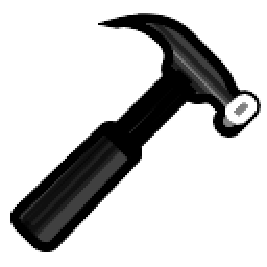
\includegraphics[width=1.5em]{Figures/exerciseLabels/hammer}} 
\newcommand{\eval}{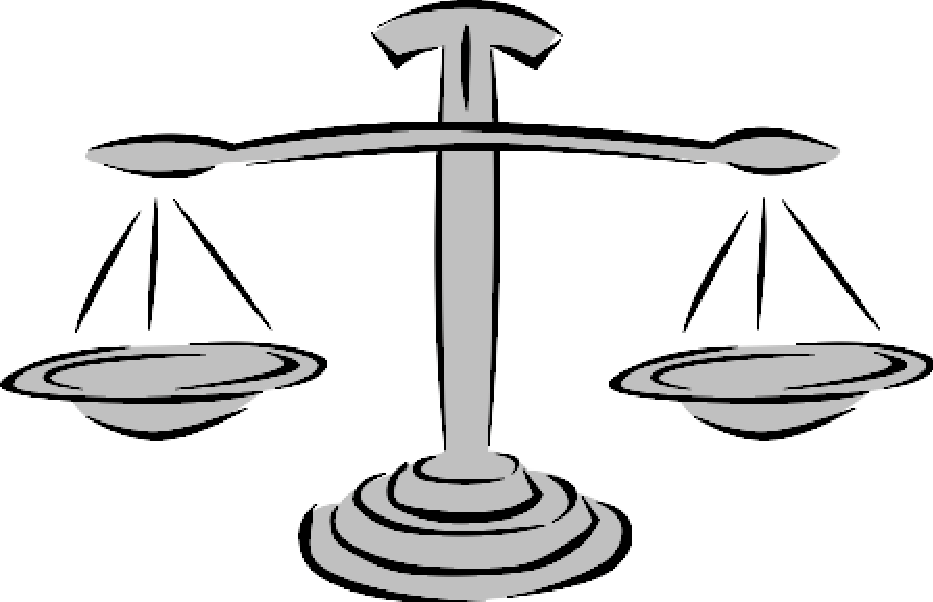
\includegraphics[width=1.5em]{Figures/exerciseLabels/scales}} 

\renewenvironment{definition}{\begin{defin}}{\end{defin}}
\renewenvironment{example}{\begin{examp}}{\end{examp}}
\newenvironment{exercise}[1][\appn]{\begin{thmexercise}\ %
    \checkoddpage
    \ifcpoddpage \reversemarginpar \fi
    \marginpar{\hfill #1}%
    \renewcommand{\theenumi}{\alph{enumi}}%
}
{\renewcommand{\theenumi}{\roman{enumi}}%
 \end{thmexercise}}

\newcommand{\chinbox}[1]{%
  \fbox{\parbox[t]{4.5in}{\textsc{Note to Self:} 
      \begin{center}
        #1
      \end{center}}}}

%% counters for use in pki.tex
%% had to be added here to allow piecemeal compilation of book.tex
\newcounter{count} \newcounter{restart} 

%%===Index related commands=====
%% main index
\newcommand{\mainindex}[1]{\index{book}{#1}}
%% symbol index
\newcommand{\symindex}[1]{\index{symbol}{#1}}

%% create the index
% \makeindex
\makeindex{symbol}
\makeindex{book}


\begin{document}
% %% get table/figure numbers to print properly in float lists
% \renewcommand*\l@figure{\@dottedtocline{1}{1.5em}{1in}}
% \renewcommand*\l@table{\l@figure}



\title{Transition Systems, Access Control, Security, and Trust: A
  Logical Approach%  \\
% \ \\ \textsc{Draft: Do Not Distribute }
}

\author{Shiu-Kai Chin and Susan Older}

\maketitle


%%%% Now to the real stuff...
\frontmatter
\thispagestyle{empty}

\begin{center}
  \textit{To the engineers and computer scientists who design and
    deliver the systems on which we depend} \\
\end{center}

\clearpage

\newcommand{\name}[1]{\ensuremath{\textit{#1}}}
\newcommand{\filename}[1]{\ensuremath{\mathtt{#1}}}
\newcommand{\rulespace}{\vspace*{2em}}


\newcommand{\pair}[1]{\ensuremath{\langle #1\rangle}}
%\newcommand{\annd}{\ensuremath{\ \&\ }}
\newcommand{\annd}{\ensuremath{\textrm{ and }}}
% \newcommand{\orr}{\ensuremath{\textrm{ or }}}
\newcommand{\pow}[1]{\ensuremath{\mathcal{P}(#1)}}
\newcommand{\set}[1]{\ensuremath{\{#1\}}}
\newcommand{\midset}[2]{\ensuremath{\set{#1 \mid #2}}}
\newcommand{\arrow}{\ensuremath{\rightarrow}}
\newcommand{\id}[1]{\ensuremath{\textsf{id}_{#1}}}
\newcommand{\subst}[3]{\ensuremath{{#1}\boldsymbol{[}#2\boldsymbol{/}#3\boldsymbol{]}}} 

%% For mathematical proofs with ``reasons'' on each step
\newenvironment{mathprf}
  {\begin{displaymath}\begin{array}{rcll}}{\end{array}\end{displaymath}}
\newcommand{\why}[1]{\ensuremath{\quad \text{#1}}}

%% for conventions (spelled out explicitly in text)
\newenvironment{convention}{\begin{description} \item[\textit{Convention:}
    ]}{\end{description}} 

\newcommand{\readernote}[2]{\noindent\shadowbox{\parbox{.95\textwidth}{%
      \begin{description} \item[\textit{#1:}] #2 \end{description}}}}



\newenvironment{indentedExample}{\begin{example}\ \begin{list}{}{}\item }{\end{list}\end{example}}

%\newenvironment{indentedExample}{\begin{example}}{\end{example}}
% for grammars

\newcommand{\isa}{\ensuremath{\; {:}{:}{=} \;}}
\newcommand{\goesto}{\ensuremath{\leadsto}}
%\newcommand{\ora}{\ensuremath{\;\mid\;}}
\newcommand{\ora}{\ensuremath{\;/\;}}
%\newcommand{\syncat}[1]{\hbox{\textcolor{red}{\sc$\langle$#1$\rangle$}}}
%\newcommand{\syncat}[1]{\hbox{{ \sc$\langle$#1$\rangle$}}}
%\newcommand{\syncat}[1]{\hbox{{ \bf #1 }}}
\newcommand{\syncat}[1]{\ensuremath{\textbf{#1}}\xspace}

% Miscellaneous

\newcommand{\defined}{\ensuremath{\quad \triangleq \quad}}
\newcommand{\defn}{\ensuremath{\stackrel{\mathrm{def}}{=}}}


\newcommand{\assign}{\ensuremath{:=}}

%%% for hiding self comments
%\renewcommand{\suebox}[1]{}
%\renewcommand{\chinbox}[1]{}

\newcommand{\key}[1]{\textbf{#1}}

% encryption

\newcommand{\encrypt}[2]{\ensuremath{\mathit{encrypt}(#2,#1)}}
\newcommand{\cat}[1]{\ensuremath{\langle\!\langle #1 \rangle \! \rangle}}

% Syntactic sets
\newcommand{\PName}{\ensuremath{\textbf{PName}}\xspace}
\newcommand{\PExp}{\ensuremath{\textbf{Princ}}\xspace}
\newcommand{\PropVar}{\ensuremath{\textbf{PropVar}}\xspace}
\newcommand{\LExp}{\ensuremath{\textbf{Form}}\xspace}
\newcommand{\LabelConst}{\ensuremath{\textbf{SecLabel}}\xspace}
\newcommand{\Level}{\ensuremath{\textbf{SecLevel}}\xspace}
\newcommand{\IntLabelConst}{\ensuremath{\textbf{IntLabel}}\xspace}
\newcommand{\IntLevel}{\ensuremath{\textbf{IntLevel}}\xspace}
% \newcommand{\PName}{\ensuremath{\textbf{\textsc{PName}}}\xspace}
% \newcommand{\PExp}{\ensuremath{\textbf{\textsc{Princ}}}\xspace}
% \newcommand{\PropVar}{\ensuremath{\textbf{\textsc{PropVar}}}\xspace}
% \newcommand{\LExp}{\ensuremath{\textbf{\textsc{Form}}}\xspace}
%\newcommand{\LExp}{\ensuremath{\textbf{\underline{Form} }}}
%\newcommand{\privs}{\ensuremath{\mathit{privs}}}
%\newcommand{\Targ}{\ensuremath{\mathcal{T}}}


% Principals
\newcommand{\with}{\ensuremath{\;\&\;}}
\newcommand{\quoting}{\ensuremath{\;|\;}}
\newcommand{\for}[1]{\ensuremath{\;\textsf{for}_{#1}\;}}

% Logical expressions
\newcommand{\has}{\ensuremath{\textsf{ has }}}
\newcommand{\says}{\ensuremath{\text{\footnotesize \textsf{ says }}}}
\newcommand{\controls}{\ensuremath{\text{\footnotesize \textsf{ controls }}}}
\newcommand{\serves}{\ensuremath{\textsf{ serves }}}
\newcommand{\speaksfor}{\ensuremath{\Rightarrow}}
\newcommand{\then}{\;\supset\;}
\newcommand{\phiplus}{\ensuremath{\varphi^{+}}}
% SKC - added syntactic sugar for ``represents''
\newcommand{\rreps}{\ensuremath{\text{\footnotesize \textsf{reps} }}}
\newcommand{\reps}[3]{\ensuremath{{#1} \text{\footnotesize \textsf{
          reps }}{#2}{\text{\footnotesize \textsf{ on }}}{#3}}}
\newcommand{\controlsandsays}{\ensuremath{\textsf{ controls+says }}}
\newcommand{\rp}[2]{\ensuremath{{#1} {\text{\footnotesize \textsf{
          reps }}}{#2}{\text{\footnotesize \textsf{ on }}}}}
\newcommand{\slv}[1]{\ensuremath{\text{\textsf{ slev}}(#1)}}
\newcommand{\ilv}[1]{\ensuremath{\text{\textsf{ ilev}}(#1)}}


% Semantics
\newcommand{\struct}[1]{\ensuremath{\langle {#1} \rangle}}
\newcommand{\krip}[1]{\ensuremath{\langle {#1} \rangle}}

\newcommand{\E}[1]{\ensuremath{\mathcal{E}_{\mathcal{M}}[\![#1]\!]}}
\newcommand{\Ee}{\ensuremath{\mathcal{E}_{\mathcal{M}}}}
\newcommand{\Em}[2]{\ensuremath{\mathcal{E}_{#2}[\![#1]\!]}}

%% for actions: 
%%   \actionit puts contents into textit mode
\newcommand{\action}[1]{\ensuremath{\langle #1 \rangle}}
\newcommand{\actionit}[1]{\ensuremath{\langle \textit{#1} \rangle}}

\newcommand{\sig}[1]{\ensuremath{\mathit{Signature}_{#1}}}

\newcommand{\mssmeet}{\ensuremath{\curlywedge}}
\newcommand{\mssbar}{\ensuremath{\|}}
\newcommand{\below}{\ensuremath{\leq}}

\newcommand{\eqmod}[1]{\ensuremath{\approx_{#1}}}

% Derivability

\newcommand{\infrule}[2]
   {\ensuremath{{\textstyle #1}\over{\textstyle #2}}}

\newcommand{\infname}[1]{\textit{#1}}

\newcommand{\irule}[3]
    {\ensuremath{\infname{#3}\quad {\displaystyle \frac{#1}{#2}}}}

\newcommand{\displaynewrule}[3]
{\begin{displaymath}
  \colorbox{LightGray}{\irule{#1}{#2}{#3}}
%  \colorbox{SpringGreen}{\irule{#1}{#2}{#3}}
\end{displaymath}}

\newcommand{\displaycorerule}[4]
{\begin{displaymath}
  \colorbox{lightgray}{\irule{#1}{#2}{#3}{#4}}
%  \colorbox{SkyBlue}{\irule{#1}{#2}{#3}{#4}}
\end{displaymath}}

\newcommand{\displaycoredef}[1]
{\begin{displaymath}
    \colorbox{lightgray}{\ensuremath{#1}}
%  \colorbox{SkyBlue}{\ensuremath{#1}}
\end{displaymath}}

%% Assorted notation for RBAC
\newcommand{\inherits}{\ensuremath{\,\succeq\,}}   % role inheritance
\newcommand{\Users}{\ensuremath{\mathit{Users}}}
\newcommand{\Perms}{\ensuremath{\mathit{Perms}}}
\newcommand{\Roles}{\ensuremath{\mathit{Roles}}}
\newcommand{\Sessions}{\ensuremath{\mathit{Sessions}}}
\newcommand{\SSD}{\ensuremath{\mathit{SSD}}}
\newcommand{\DSD}{\ensuremath{\mathit{DSD}}}
\newcommand{\ausers}{\ensuremath{\mathit{auth\_users}}}
\newcommand{\aperms}{\ensuremath{\mathit{auth\_perms}}}
\newcommand{\suser}{\ensuremath{\mathit{user}}}
\newcommand{\sroles}{\ensuremath{\mathit{roles}}}


% Generalized addresses
% \newcommand{\genAddr}[2]{\ensuremath{\langle\negmedspace\langle #1
%     \rangle\negmedspace\rangle}{\mid #2}}
\newcommand{\segName}[1]{\ensuremath{\langle\negmedspace\langle #1
    \rangle\negmedspace\rangle}}

%% address-descriptor location for named segment
\newcommand{\adLoc}[1]{\ensuremath{|\!| #1 |\!|}}
\newcommand{\segLoc}[1]
    {\ensuremath{\langle\!\!\langle #1 \rangle\!\!\rangle}}
\newcommand{\genAddr}[2]{\ensuremath{[ #1:#2 ]}}
\newcommand{\genAddrPair}[2]{\ensuremath{(#1,#2)}}

%% Formal proof environment

\newenvironment{formalProof}
{\begin{center}\small\begin{tabular}{ll}}{\end{tabular}\end{center}} 


%% Alternate Formal proof environment



\newenvironment{tabProof}{\begin{center}\footnotesize\begin{tabular}{r
        >{$}p{3.2in}<{$}p{1.0in}}}{\end{tabular}\end{center}}  
\newenvironment{tabProof2}{\begin{center}\footnotesize\begin{tabular}{r >{$}p{2.7in}<{$}p{1.5in}}}{\end{tabular}\end{center}} 

% if then else
\newcommand{\ite}[3]
   {\ensuremath{#1 \rightarrow #2 \mid #3}}

%%  Macro(s) for section summaries
\newcommand*{\summproblem}[1]{\def\fromsummproblem{#1}}
\newcommand*{\summanalysis}[1]{\def\fromsummanalysis{#1}}
\newcommand*{\summresults}[1]{\def\fromsummresults{#1}}

\newcommand{\missing}{\textsc{Missing Component}}
\summproblem{\missing}
\summanalysis{\missing}
\summresults{\missing}

\newcommand{\makesummary}
  {%\section{Summary} 
    \begin{enumerate}
    \item \textsc{What is the problem?}
%      \begin{quote}
%        \it What is the purpose of my thinking?  What precise
%        question am I trying to answer?  Within what point of view am I
%        thinking?
%      \end{quote}
%      \ \\ 

      \fromsummproblem
    \item  \textsc{How am I analyzing the problem?}
%      \begin{quote}
%        \it What am I taking for granted, and what assumptions am
%        I making? What information am I using?  How am I interpreting
%        that information?  What concepts or ideas are central to my
%        thinking? 
%      \end{quote}
%      \ \\ 

      \fromsummanalysis
    \item \textsc{What are the results?}
%      \begin{quote}
%        \it What conclusions am I coming to?  If I accept the
%        conclusions, what are the implications?  What would the
%        consequences be, if I put my thought into action?
%      \end{quote}
%      \ \\ 

      \fromsummresults
    \end{enumerate}

  \summproblem{\missing}
  \summanalysis{\missing}
  \summresults{\missing}
    
}


%----redefine implication as horseshoe instead of arrow--------

\renewcommand{\implies}{\supset}
\newcommand{\believes}{\ensuremath\textsf{ believes }}

%%% Local Variables: 
%%% mode: latex
%%% TeX-master: "book"
%%% End: 


%% from proofreader: table of contents should be on page vii
\setcounter{page}{6}

\tableofcontents
\listoftables
\listoffigures


\chapter*{Preface}

This manual is meant to be a companion to the textbook \emph{Access
  Control, Security, and Trust: A Logical Approach}, \cite{ACST}, by
Chin and Older. We have embedded the syntax and semantics of the
access-control logic in \cite{ACST} in the Cambridge Higher-Order
Logic (HOL-4) theorem prover, \cite{HOL}. Additionally, we have
defined inference rules in HOL corresponding to the inference rules in
\cite{ACST}.


%%% Local Variables:
%%% mode: latex
%%% TeX-master: "aclHOLManual"
%%% End:

% LocalWords:  emph vspace hfill Archidamus ldots textsc Kananaskis 7 RMAs AFRL
% LocalWords:  HOL Kananaskis

\mainmatter
%introduction
\documentclass[../../main/main.tex]{subfiles}

\pagenumbering{arabic}

\begin{document}
\glsresetall

\chapter{Introduction}
Some text here.\cite{ChinOlder} testing citations from the references.

      %%%%%%%%%%%%%%%%%%%% Section Motivation %%%%%%%%%%%%%%%%%%%%%%
\section{Motivation}\;abel{sec:intro:motivation}
\subsection{Systems Are Everywhere}
\subsection{CIA: Confidentiality, Integrity, and Accountability}


\section{This Master Thesis}\label{sec:thismasterthesis}
\glsresetall
This master thesis describes a method for designing secure systems.  The method is called \glsfirst{csbd}. \glsunset{csbd}  \glsname{csbd} has been successfully demonstrated on automated systems such as ... and ....  But, until this research, it has not been demonstrated on non-automated, human-centered systems.  

Systems span the range of fully automated to fully non-automated.  This master thesis focuses on one end of this range: non-automated, human-centered systems.


\begin{itemize}
\item The first question addressed in this master thesis is whether \gls{csbd} could be successfully applied to non-automated, human-centered systems.  This is the primary objective.  An example of a non-automated, human-centered system is the patrol base operations defined in the United States Army Ranger Handbook\cite{rangermanual}.   Patrol base operations exemplify a non-automated, human-centered system wherein security is critical to mission success.  In this master thesis, the results of applying CSBD to patrol base operations is discussed. 

\item The patrol base operations are also an example of a predefined system.  This means that this thesis also addresses the question of whether CSBD could be successfully applied to a pre-designed, non-automated, human-centered system.  This is important because many such systems in use today are already designed and implemented.  CSBD demonstrates that it can verify and document the security properties of current, in-use systems.  

\item These thesis describes a hierarchy of secure state machines (SSMs) used to model the patrol base operations.  This approach demonstrates that formal methods can be applied to large scale and complicated systems.  The hierarchy manages patrol base operations by successful levels of decreasing abstraction.  Each level in the hierarchy consists of one or more SSMs.  Each SSM is modularized and models one aspect of the patrol base operations at one level of abstraction.  The levels and modules are connected together by an OMNI level, all-seeing, principal.  Each module only needs to be aware of this OMNI level principal.  They do not need to be aware of the details of any other module.  With this divide-and-conquer approach, CSBD can be readily applied to large and complicated systems.

\item The successful application of CSBD to patrol base operations also suggests its use in combining automation with human-centered systems.  The approach employed by this master thesis involves describing the patrol base operations as a hierarchy of secure state machines.  This hierarchy has the property that it is easy to demonstrate security properties of the system, which is the goal of CSBD.  But, it also has the property that it describes the patrol base operations as a system that is amiable to automation.  Such automations of pre-defined non-automated, human-centered systems could include, for example, accountability systems for tracking supplies and personal.  In the not-so-distant future, the military, in particular, will most likely seek tracking and accountability systems for pre-existing, non-automated military operations.  These systems, like all security-sensitive military systems, should be designed according to NIST 800-160 standards.  These standards require the formal verification and documentation provided by CSBD and demonstrated in this thesis.   

\end{itemize}


\end{document}

\part{Preliminaries}


\chapter{Reasoning about Access Control}
\label{chap:access-control}

% ---- this points LaTeX to book.tex ---- 
% Local Variables: 
% TeX-master: "book"
% End:


\chapter{Reasoning about Transitions}
\label{chap:transitions}

% ---- this points LaTeX to book.tex ---- 
% Local Variables: 
% TeX-master: "book"
% End:


\chapter{Reasoning Using the Higher Order Logic Theorem Prover\\
\small{\redtext{\textsc{Do Not Distribute}}}}
\label{chap:hol}

% \chinbox{
%   \begin{itemize}
%   \item HOL as a CAD tool
%   \item HOL is stable
%   \item Chapter meant to provide reading knowledge, not a user's manual
%   \item Distinction between meta and object levels
%   \end{itemize}
% }

\paragraph*{Why Use Theorem Provers?}

Human error is ever present in even the simplest of calculations. As
security and integrity are crucial to critical applications such as
command-and-control, and designs have a myriad of detail, the chances
of getting every detail absolutely correct is vanishingly
small. 

The need to handle a large number of design and verification details
is not new. This is the same situation faced by design and
verification engineers of very large-scale integrated (VLSI)
circuits. Modern microprocessors have billions of transistors. Even
the simple-sounding task of accounting for all the connections among a
microprocessor's transistors is completely impractical using manual
methods alone. Computer-assisted design (CAD) tools for design-rule
checking (checking to make sure that circuit layouts satisfy rules
such as minimum width and spacing constraints between wires) and logic
to layout verification (checking that the electrical behavior of
transistor-level circuits is consistent with the logical behavior
described by logic schematics), are essential for VLSI hardware
design.

Assuring system security and integrity requires consistency among
policies and implementations across multiple levels of abstraction:
from high-level organizational policies down to the control of
physical memory. Managing and guaranteeing consistency among
access-control policies, trust assumptions, and interpretation of
messages and certificates is beyond manual methods.

Computer-assisted reasoning tools, such as proof checkers and theorem
provers, for checking consistency among policies and implementations,
have an analogous role to CAD tools in hardware design. Both are
antidotes to human error, self-delusion, and the complexity of large
numbers of design details. 

There are several advantages to using theorem provers and proof checkers.
\begin{enumerate}
\item Formal verification of proofs of theorems provides high
  assurance and confidence of correctness to designers, customers, and
  certifiers.
\item All the details of definitions and proofs are disclosed.
\item Properties, expressed as theorems, are both precise and
  accurate.
\item Theorem provers and proof checkers enable rapid checking, reuse,
  and reproduction of results by third parties uninvolved in the
  original design and verification effort.
\end{enumerate}

\paragraph*{Why HOL?}

There are many proof checkers and theorem provers, such as HOL, Coq,
Nuprl, and ACL2. Each have a long history of use and stability. We use
HOL for the following reasons.
\begin{enumerate}
\item HOL as collection of functions, in the ML (meta-language)
  programming language and interpreter, is highly flexible in terms of
  supporting user-defined inference rules and decision
  procedures. This enables us to extend HOL to include the
  access-control logic along with its inference rules.
\item HOL supports both forward inference (starting from theorems and
  proving new theorems) as well as backwards reasoning (starting from
  goals and proving theorems). HOL's forward inference rule capability
  mimics the proof style used in the access-control logic. HOL's
  backward reasoning capability allows for complicated proofs to be
  done efficiently due to the suppression of detail.
\item HOL has an extensive library of contributed libraries and
  examples. HOL's libraries enable users to build upon a sound
  foundation provided by others. This was the case when we developed
  the access-control logic.
\end{enumerate}

This chapter on HOL is not a tutorial or a complete description of
HOL. The HOL system comes with excellent documentation
(\emph{Tutorial, Description, Logic,} and \emph{Reference}). The
purpose of this chapter is to give a reading comprehension of HOL so
that readers can comprehend the access-control logic and operational
semantics in HOL. Our intent is to enable readers to both comprehend
and reproduce our results. By so doing, readers are able to create
their own extensions to the logic and inference rules related to the
access-control logic and transition systems.

\section{Terms and Types}
\label{sec:terms-types}

\paragraph*{ML and HOL}

HOL is implemented using the ML functional language. ML is a
\emph{strongly typed} language.  This means that every well-formed
expression in ML has a type. The advantage of strongly-typed languages
is the detection and avoidance of nonsensical expressions and
formulas.  For example, the expression $1 + 2 = 3$ is well typed,
assuming ``+'' denotes addition.

The relation between ML and HOL is this: \emph{HOL is implemented
  within ML as a set of types and functions that manipulate HOL
  objects}. More precisely, HOL \emph{objects} are \emph{HOL terms or
  formulas}, \emph{HOL types,} and \emph{HOL theorems}. HOL objects
are manipulated by ML functions. ML is the \emph{meta-language} that
constructs and deconstructs HOL objects.

\paragraph*{HOL Terms and ML Types}

\begin{center}
  \begin{table}[ht]
    \centering
    \begin{tabular}{|l|l|l|l|} \hline
\multicolumn{4}{|c|}{ } \\
\multicolumn{4}{|c|}{\bf Terms of the HOL Logic} \\
\multicolumn{4}{|c|}{ } \\
{\it Kind of term} & {\it \HOL{} notation} &
{\it Standard notation} &
{\it Description} \\ \hline
 & & & \\
Truth & {\small\verb|T|} & $\top$ & {\it true}\\ \hline
Falsity & {\small\verb|F|} & $\bot$ & {\it false}\\ \hline
Negation & {\small\verb|~|}$t$ & $\neg t$ & {\it not}$\ t$\\ \hline
Disjunction & $t_1${\small\verb|\/|}$t_2$ & $t_1\vee t_2$ &
$t_1\ ${\it or}$\ t_2$ \\ \hline
Conjunction & $t_1${\small\verb|/\|}$t_2$ & $t_1\wedge t_2$ &
$t_1\ ${\it and}$\ t_2$ \\ \hline
Implication & $t_1${\small\verb|==>|}$t_2$ & $t_1\imp t_2$ &
$t_1\ ${\it implies}$\ t_2$ \\ \hline
Equality & $t_1${\small\verb|=|}$t_2$ & $t_1 = t_2$ &
$t_1\ ${\it equals}$\ t_2$ \\ \hline
$\forall$-quantification & {\small\verb|!|}$x${\small\verb|.|}$t$ &
$\uquant{x}t$ & {\it for\ all\ }$x: t$ \\ \hline
$\exists$-quantification & {\small\verb|?|}$x${\small\verb|.|}$t$ &
$\equant{x}\ t$ & {\it for\ some\ }$x: t$ \\ \hline
$\hilbert$-term & {\small\verb|@|}$x${\small\verb|.|}$t$ &
$\hquant{x}t$ & {\it an}$\ x\ ${\it such\ that:}$\ t$ \\ \hline
Conditional & {\small\verb|if|} $t$ {\small\verb|then|} $t_1$
              {\small\verb|else|} $t_2$ &
$(t\rightarrow t_1, t_2)$ & {\it if\ }$t${\it \ then\ }$t_1${\it\ else\ }$t_2$
 \\ \hline
\end{tabular}

\caption{Terms in HOL}
\label{tab:logic-table}
\end{table}
\end{center}

Table~\ref{tab:logic-table} taken from \cite{HOLTutorial}, shows the
representation of HOL terms in ASCII, in standard notation, and with a
brief description of each term. The ASCII representation is what we
put into the HOL system as part of the ML interpreter.

Terms or well-formed formulas in HOL are predicate calculus terms
where (1) variables can range over predicates and functions---hence
the characterization of HOL as \emph{higher order}, and (2) all HOL
terms have a \emph{type}. There are various pretty printers supporting
HOL. Nevertheless, HOL makes use of ASCII characters to represent
elements such as $\forall$ (universal quantification) and $\in$ (set
membership).

Terms in HOL appear in ML as formulas surrounded by double backwards
quotes.  As examples, the formulas $p \wedge q$ (the conjunction of
$p$ and $q$) and $\forall x.P x$ (for all $x$ $P(x)$ is true), are
shown in HOL Session \ref{session:term1} below.
\begin{session}
\label{session:term1}
\begin{verbatim}

- ``p /\ q``;
> val it = ``p /\ q`` : term
- ``! x. P(x)``;
<<HOL message: inventing new type variable names: 'a>>
> val it = ``!x. P x`` : term
\end{verbatim}
\end{session}
The session above exemplifies an \emph{interactive} session in HOL,
where user inputs are on lines starting with a dash \texttt{-} and
ending with a semicolon \texttt{;}. System responses are on lines
starting with \texttt{>}.

In the session above, we entered \small{\verb|``p /\ q``|} and ML
responded with
\begin{verbatim}
> val it = ``p /\ q`` : term
\end{verbatim}
The response means that the \emph{ML value} of the input expression is
\small{\verb|``p /\ q``|}, which has \emph{\textbf{ML
  type}} \textrm{:term}. The same thing can be said about the response
\begin{verbatim}
> val it = ``!x. P x`` : term
\end{verbatim}
The input expression \small{\verb|``! x. P(x)``|} has the
ML type \texttt{:term}, which is the same ML type as
\small{\verb|``p /\ q``|}.

The only remaining explanation needed is to explain the meaning of:
\begin{verbatim}
<<HOL message: inventing new type variable names: 'a>>
\end{verbatim}
To do this, we need to talk about \emph{\textbf{HOL types}}, i.e.,
types in HOL as opposed to types in ML. The key concept here is to
distinguish between \emph{meta-level types} in ML versus
\emph{object-level types} in HOL. Viewed from the ML perspective, all
HOL formulas are of ML type \texttt{:term}.  Usually, we are concerned
about the types of objects in HOL, i.e., at the object level within
HOL.

\paragraph*{HOL Types}

When we say ``HOL types'', we mean the types of formulas within HOL,
as opposed to ML. As a concrete illustration, consider again the HOL
formula $p \wedge q$, where $\wedge$ denotes conjunction and is a
boolean operator operating on two boolean terms $p$ and $q$.

If we input \small{\verb|``p /\ q``|} into HOL, but this
time with HOL set to display HOL types, we get
Session~\ref{session:term2} shown below.
\begin{session}
  \label{session:term2}
\begin{verbatim}

- ``p /\ q``;
> val it = ``(p :bool) /\ (q :bool)`` : term
\end{verbatim}
\end{session}
As before, the above session shows that within ML that
\small{\verb|``p /\ q``|} evaluates to an ML value of type
\texttt{:term}.  Additionally, \emph{inside the quotes}, we see that
terms $p$ and $q$ have \emph{\textbf{HOL type}} \texttt{:bool}. To see
what the HOL type of \small{\verb|``p /\ q``|} is, we use
the ML function \texttt{type\_of}, whose ML type signature is
\texttt{: term -> hol\_type}. Session~\ref{session:term3} shows the ML
type signature of \texttt{type\_of} and the result of applying it to
\small{\verb|``p /\ q``|}.
\begin{session}
  \label{session:term3}
\begin{verbatim}

> val it = fn : term -> hol_type
- type_of ``p /\ q``;
> val it = ``:bool`` : hol_type
\end{verbatim}
\end{session}
The above result says that the HOL type of
\small{\verb|``p /\ q``|} is \texttt{:bool}, which makes
perfect sense.  Again, notice that this is \emph{HOL type}
\texttt{:bool} as opposed to ML type \texttt{:term}. This is another
illustration of the difference between operating at the \emph{object
  level} in HOL versus the \emph{meta level} in ML.

We can see this distinction with an even simpler example. Consider the
numeral 1. 1 entered without HOL quotes is the ML integer value 1,
i.e. \texttt{1 : int}.  In contrast, \texttt{``1``}
is the HOL \emph{natural number} \texttt{1 : num}.  This is shown
below in Session~\ref{session:term4}.
\begin{session}
  \label{session:term4}
\begin{verbatim}

- 1;
> val it = 1 : int
- ``1``;
> val it = ``(1 :num)`` : term
\end{verbatim}
\end{session}
The above shows the difference between the ML meta value 1 versus the
HOL object \texttt{``1``}.

\subparagraph*{HOL Type Variables}

HOL supports polymorphism through the use of \emph{type
  variables}. Type variables in HOL are similar to type variables in
functional languages such as ML and Haskell. Type variables in HOL all
start with a single forward quote mark \texttt{'}.  For example, the
HOL type \texttt{``:'a``} is a type variable (pretty printed as
$\alpha$).
\begin{session}
  \label{session:term5}
\begin{verbatim}

- ``:'a``;
> val it = ``:'a`` : hol_type
\end{verbatim}
\end{session}

As in functional languages, type variables and polymorphism allow
\emph{the same definition to be used on different types.}  The
advantages include simplicity derived from the reuse of definitions as
well as abstraction derived from properties of definitions that apply
over different types.  

For example, consider the pair \texttt{``(1,F)``}, i.e., the pair of
HOL terms \texttt{``1``} and \texttt{``F``} where \texttt{1} has HOL
type \texttt{``:num``} and \texttt{F} is the HOL value \emph{false}
with HOL type \texttt{``:bool``}. Session~\ref{session:term6} shows
that the HOL type of \texttt{``(1,F)``} is the Cartesian product $num
\times bool$, written in ASCII as \texttt{``:num \# bool``}.
\begin{session}
\label{session:term6}
\begin{verbatim}

- ``(1,F)``;
> val it = ``((1 :num),F)`` : term
- type_of ``(1,F)``;
> val it = ``:num # bool`` : hol_type
\end{verbatim}
\end{session}
HOL, as most functional languages do, has two accessor functions for
retrieving the first or second elements of pairs. In HOL, these
functions are \texttt{FST} and \texttt{SND}, respectively. In
Session~\ref{session:term7} below, we see that the HOL type of
\texttt{``FST``} is \texttt{``:'a \# 'b -> 'a``}. Specifically,
\texttt{FST} takes as an input a HOL pair (Cartesian product) where
the first element is of type \texttt{``:'a``}, and the second element
is of type \texttt{``:b``}. The value returned is the first element of
the pair, which is of type \texttt{``:'a``}.  Similarly,
\texttt{``SND``} also takes takes as an input a HOL pair (Cartesian
product) where the first element is of type \texttt{``:'a``}, and the
second element is of type \texttt{``:b``}. The value returned is the
second element of the pair, which is of type \texttt{``:'b``}.

\texttt{FST} and \texttt{SND} being polymorphic, can be applied to
pairs of any type. When applied to a specific pair, the type variables
\texttt{``:'a``} and \texttt{``:'b``} are instantiated to the
corresponding types of the specific pair. In
Session~\ref{session:term7} below, we see that the HOL type of
\texttt{``FST(1,F)``} is \texttt{``:num``} and the HOL type of
\texttt{``SND(1,F)``} is \texttt{``:bool``}. Thus, types
\texttt{``:'a``} and \texttt{``:'b``} were instantiated to types
\texttt{``:num``} and \texttt{``:bool``}, respectively.
\begin{session}
  \label{session:term7}
\begin{verbatim}

- ``FST``;
<<HOL message: inventing new type variable names: 'a, 'b>>
> val it =
    ``(FST :'a # 'b -> 'a)``
     : term
- ``SND``;
<<HOL message: inventing new type variable names: 'a, 'b>>
> val it =
    ``(SND :'a # 'b -> 'b)``
     : term
- type_of ``FST(1,F)``;
> val it = ``:num`` : hol_type
- type_of ``SND(1,F)``;
> val it = ``:bool`` : hol_type
\end{verbatim}

\end{session}

Based on the above examples, we can explain more fully the HOL message
in Session~\ref{session:term1}. Taking advantage of displaying types
explicitly when entering \texttt{``!x.P x``}, we see the HOL types of each component as shown below in Session~\ref{session:term8}:
\begin{session}
\label{session:term8}
\begin{verbatim}

- ``!x.P x``;
<<HOL message: inventing new type variable names: 'a>>
> val it = ``!(x :'a). (P :'a -> bool) x`` : term
\end{verbatim}
\end{session}
What Session~\ref{session:term8} shows is HOL will make variables,
predicates, and functions as general as possible by assigning type
variables whenever possible. In the above case, variable $x$ is
assigned the HOL type variable \texttt{``:'a``}.  As the type of
$P\;x$ ultimately must be boolean, the HOL type of predicate
\texttt{``P``} must be \texttt{``:'a -> bool``}, i.e., a function
operating on inputs of HOL type \texttt{``:'a``} and returning boolean
values.  The HOL message informs us that it used type variable
\texttt{``:'a``} when evaluating the expression \texttt{``!x.P x``}.

\section{Constructing and Deconstructing HOL Terms}
\label{sec:construction-deconstruction}

One of the benefits of using systems such as HOL is the ability to
extend the syntax and semantics of HOL \emph{safely}, i.e., in ways
that guarantee logical soundness.  This includes the capability to
introduce new syntax and semantics, such as the syntax of our
access-control logic and its associated Kripke semantics. We can also
introduce the inference rules of the access-control logic as sound HOL
inference rules.

As we will see shortly, inference rules in HOL are ML functions that
return HOL theorems as results. Central to inference rules is the
capability to construct and deconstruct HOL terms using built-in and
customized ML functions.  In this section, we will show how this is
done.

\begin{table}[tb]
  \centering
  \begin{tabular}{|l|l|l|l|l|}
    \hline
    \multicolumn{5}{|c|}{\textbf{ML Functions on HOL Terms}}\\
    \emph{Kind of term} & \emph{HOL notation} & \emph{Predicate} & \emph{Deconstructor} & \emph{Constructor}\\
    \hline
    Variable & $x$ & \small{\verb|is_var|}& \small{\verb|dest_var|}& \small{\verb|mk_var|}\\
    \hline
    HOL Type & $:ty$ & \small{\verb|is_vartype|} & \small{\verb|dest_vartype|} & \small{\verb|mk_vartype|} \\
    \hline
    Negation & {\small\verb|~|}$t$ &\small{\verb|is_neg|} & \small{\verb|dest_neg|}& \small{\verb|mk_neg|}\\
    \hline
    Disjunction & $t_1${\small\verb|\/|}$t_2$ & \small{\verb|is_disj|}& \small{\verb|dest_disj|}& \small{\verb|mk_disj|}\\
    \hline
    Conjunction & $t_1${\small\verb|/\|}$t_2$ & \small{\verb|is_conj|}& \small{\verb|dest_conj|}& \small{\verb|mk_conj|}\\
    \hline
    Implication & $t_1${\small\verb|==>|}$t_2$ & \small{\verb|is_imp|}& \small{\verb|dest_imp|}& \small{\verb|mk_imp|}\\
    \hline
    Equality & $t_1${\small\verb|=|}$t_2$ & \small{\verb|is_eq|}& \small{\verb|dest_eq|}& \small{\verb|mk_eq|}\\
    \hline
    $\forall$-quantification & {\small\verb|!|}$x${\small\verb|.|}$t$ & \small{\verb|is_forall|}& \small{\verb|dest_forall|}& \small{\verb|mk_forall|}\\
    \hline
    $\exists$-quantification & {\small\verb|?|}$x${\small\verb|.|}$t$ & \small{\verb|is_exists|}& \small{\verb|dest_exists|}& \small{\verb|mk_exists|}\\
    \hline
    $\hilbert$-term & {\small\verb|@|}$x${\small\verb|.|}$t$ & \small{\verb|is_select|}& \small{\verb|dest_select|}& \small{\verb|mk_select|}\\
    \hline
    Conditional & {\small\verb|if|} $t$ {\small\verb|then|} $t_1$
              {\small\verb|else|} $t_2$ &\small{\verb|is_cond|} & \small{\verb|dest_cond|}& \small{\verb|mk_cond|}\\
    \hline
    Function application & $t_1${\small{\verb| |}$t_2$} & \small{\verb|is_comb|}& \small{\verb|dest_comb|}& \small{\verb|mk_comb|}\\
    \hline
    Lambda abstraction & \verb|\|$x.f$ & \small{\verb|is_abs|}&\small{ }\verb|dest_abs|&\small{\verb|mk_abs|}\\
    \hline
  \end{tabular}
  \caption{Predicates, Deconstructor, and Constructor Functions}
  \label{tab:constructors-deconstructors}
\end{table}

Table~\ref{tab:constructors-deconstructors} show the predicates
(tests), deconstructor, and constructor functions for common HOL
formulas. When interacting directly with HOL through the ML
interpreter, we can input directly the HOL terms we want. However, in
the case where we build specialized inference rules, we need to be
able to deconstruct HOL terms and reassemble them in useful ways. Our
first example shows how to deconstruct an example HOL term.

\begin{example}
  Suppose we wish to take HOL terms of the form $t_1 \wedge t_2$ and
  reassemble them to form the term $t_2 \wedge t_1$.  The steps we
  take are the following:
  \begin{enumerate}
  \item deconstruct $t_1 \wedge t_2$ using \small{\verb|dest_conj|} to
    get the individual components $t_1$ and $t_2$, then
  \item construct the term $t_2 \wedge t_1$ using $t_1$ and $t_2$ with
    \small{\verb|mk_conj|}.
  \end{enumerate}

  As an illustration, suppose we have the HOL term
  \small{\verb|``p /\ q``|}. We use the steps above in the following
  HOL session.
  \begin{session}
    \label{session:term9}
\begin{verbatim}

- val (t1,t2) = dest_conj ``p /\ q``;
> val t1 = ``(p :bool)`` : term
  val t2 = ``(q :bool)`` : term
- mk_conj (t2,t1);
> val it = ``(q :bool) /\ (p :bool)`` : term
\end{verbatim}
  \end{session}

  How do we generalize the above to a function
  \small{\verb|swap_conj|}, which operates on HOL conjunctions?
  Essentially, we parametrized the input term and use \emph{let
    expressions} to define an ML function that swaps the order of
  terms in HOL conjunctions. Consider the HOL session below.
  \begin{session}
\begin{verbatim}

- fun swap_conj term =
  let
   val (t1,t2) = dest_conj term
  in
   mk_conj(t2,t1)
  end;
> val swap_conj = fn : term -> term
- swap_conj ``p /\ q``;
> val it =
    ``(q :bool) /\ (p :bool)``
     : term
- swap_conj ``(!x:'a.P x) /\ (?y:'b.Q y)``;
> val it =
    ``(?(y :'b). (Q :'b -> bool) y) /\ 
      !(x :'a). (P :'a -> bool) x`` : term
\end{verbatim}
  \end{session}

  The above illustrates how values and functions are defined in ML as
  well as let expressions. The example shows how arbitrary
  conjunctions
\end{example}

In the next example, we show how deal with function applications,
e.g., \texttt{``P x``}.
\begin{example}
  Suppose we wish to convert HOL terms of the form
  \small{\verb|P(x) ==> Q(y)|} to \small{\verb|Q(x) ==> P(y)|}. Our
  approach is to
  \begin{enumerate}
  \item deconstruct the top-level implication to get $P(x)$ and $Q(y)$, 
  \item deconstruct both function application $P(x)$ and $Q(y)$ to get
    $P$, $Q$, $x$, and $y$, and
  \item construct the desired term using the components above.
  \end{enumerate}

  \begin{session}
\begin{verbatim}

- fun swap_imp term =
let
  val (t1,t2) = dest_imp term
  val (f1,arg1) = dest_comb t1
  val (f2,arg2) = dest_comb t2
  val t3 = mk_comb(f2,arg1)
  val t4 = mk_comb(f1,arg2)
in
  mk_imp(t3,t4)
end;
> val swap_imp = fn : term -> term
- swap_imp ``P (x:'a) ==> Q (y:'a)``;
> val it =
    ``(Q :'a -> bool) (x :'a) ==> (P :'a -> bool) (y :'a)``
     : term
\end{verbatim}
  \end{session}

  The above example show that we can develop let expressions with
  multiple value (and function) assignments.
\end{example}

HOL has many built-in infix functions such as addition \texttt{+},
conjunction \small{\verb|/\|}, etc.  We can always transform infix
relations and functions into their prefix form by pre-pending
\small{\verb|$|} to the infix function. This is shown in the session
below where we create the function $\lambda x\;y. \$\wedge x\;y$.
\begin{session}
\begin{verbatim}

- val term = ``\x y.$/\ x y``;
> val term =
    ``\(x :bool) (y :bool). x /\ y``
     : term
- type_of term;
> val it =
    ``:bool -> bool -> bool``
     : hol_type
\end{verbatim}
\end{session}

Suppose a function that is expecting one argument form is applied to an
argument with a form different than expected. What happens? For
example, suppose that \small{\verb|swap_conj|} is applied to a simple
variable?
\begin{session}
\begin{verbatim}

- swap_conj ``x``;
<<HOL message: inventing new type variable names: 'a>>
! Uncaught exception: 
! HOL_ERR
\end{verbatim}
\end{session}
The error message above is not particularly informative. We can use
the ML function \emph{mk\_HOL\_ERR} to produce error messages to help
users and developers. \emph{mk\_HOL\_ERR} takes three strings as
arguments. Typically, the first string identifies the relevant module.
The second string identifies the relevant function. The third string
is the error message itself.  The session below shows another ML
function \emph{Swap\_Conj}, which uses both \emph{swap\_conj} and
\emph{mk\_HOL\_ERR}.
\begin{session}
\begin{verbatim}

- fun Swap_Conj term =
let
 fun swap_conj x =
 let
  val (t1,t2) = dest_conj x
 in
  mk_conj(t2,t1)
 end
in
 if is_conj term then swap_conj term
 else
  (Raise
   (mk_HOL_ERR "basics" "Swap_Conj" "input not conjunction"))
end;
> val Swap_Conj = fn : term -> term
- Swap_Conj ``A /\ B``;
> val it =
    ``(B :bool) /\ (A :bool)``
     : term
- Swap_Conj ``A ==> B``;

Exception raised at basics.Swap_Conj:
input not conjunction
! Uncaught exception: 
! HOL_ERR
\end{verbatim}
\end{session}

The above session also demonstrates how \small{\verb|swap_conj|} can
be defined internally to \small{\verb|Swap_Conj|} within an ML let
statement.

\begin{exercise}[\synthesis]
  Construct the following HOL terms using ML constructor
  functions. Note: for numbers and existing functions, it is
  permissible to use their corresponding HOL terms, e.g.,
  \texttt{``5``}, \texttt{\$+}, and \texttt{LENGTH}.  All other terms,
  including variables, must be constructed using ML functions.
      \begin{align*}
        & \forall x.(P(x) \wedge Q(x))\\
        & \exists x.(P(x) \vee Q(x))\\
        & P(5) \implies Q(6)\\
        & if \; P(x) \;then \;+ \;else \;-\\
        & CONS (1,2) [(3,4);(5,6)]\\
        & LENGTH (xs:(bool)list) = 6\\
        & MAP (f:\alpha \rightarrow \beta) (xs:(\alpha)list) =
        (ys:(\beta)list)\\
        & \lambda x.x+1\\
      \end{align*}
\end{exercise}

\begin{exercise}[\synthesis]
Define a function \texttt{AndImp2Imp} that takes HOL terms of the form
$(p \wedge q) \implies r$ and returns the term $p \implies (q \implies
r)$. The desired behavior of the function is illustrated below.
\begin{session}
\begin{verbatim}

- AndImp2Imp ``(~p\/q) /\ (q /\ ~r) ==> (s = t)``;
<<HOL message: inventing new type variable names: 'a>>
> val it = ``~p \/ q ==> q /\ ~r ==> (s = t)`` : term

- AndImp2Imp ``p /\ r``;
Exception raised at hw2.AndImp2Imp:
top term not implication
! Uncaught exception: 
! HOL_ERR

- AndImp2Imp ``p ==> (r /\ s)``;
Exception raised at hw2.AndImp2Imp:
antecedent not conjunction
! Uncaught exception: 
! HOL_ERR
\end{verbatim}
\end{session}
  
\end{exercise}

\begin{exercise}[\synthesis]
Define a function \texttt{ImpImp2And} that takes HOL terms of the form
$p \implies (q \implies r)$ and returns the term $(p \wedge q)
\implies r$. The desired behavior of the function is illustrated below.
\begin{session}
\begin{verbatim}

- AndImp2Imp ``(~p\/q) /\ (q /\ ~r) ==> (s = t)``;
<<HOL message: inventing new type variable names: 'a>>
> val it = ``~p \/ q ==> q /\ ~r ==> (s = t)`` : term

- ImpImp2And(AndImp2Imp ``(~p\/q) /\ (q /\ ~r) ==> (s = t)``);
<<HOL message: inventing new type variable names: 'a>>
> val it = ``(~p \/ q) /\ q /\ ~r ==> (s = t)`` : term

- ImpImp2And ``p /\ q ==> r``;
Exception raised at hw2.ImpImp2And:
term not implication
! Uncaught exception: 
! HOL_ERR

- ImpImp2And ``p ==> (q \/ r)``;
Exception raised at hw2.ImpImp2And:
term not implication
! Uncaught exception: 
! HOL_ERR
\end{verbatim}
\end{session}
  
\end{exercise}

\section{Theorems in HOL}
\label{sec:theorems-hol}

Theorems in HOL are ML objects of type \texttt{:thm}.  Inference rules
in HOL are ML functions that return ML objects of type
\texttt{:thm}. In this introduction to forward inference in HOL, we
learn the basics of doing HOL proofs using ML inference rules. Forward
proofs, as opposed to goal-oriented (so-called backwards proofs), take
very small and precise steps. This degree of precision promotes a
clear understanding of proofs, which is a useful foundation for larger
proofs using sophisticated decision procedures.

Theorems in HOL are \emph{sequents} of the form $\Gamma \vdash
\varphi$, where $\Gamma$ and $\varphi$ are a set of boolean terms and
a boolean term, respectively. $\Gamma$ is the set of terms known as
the \emph{hypotheses} of a theorem. $\varphi$ is the conclusion.

Theorems in HOL are guaranteed to be \emph{valid} and \emph{safe}. By
valid, we mean whenever all the hypotheses in $\Gamma$ are true, the
conclusion $\varphi$ is guaranteed to be true, with no exceptions. By
safe, we mean that the implementation of HOL in ML has demonstrated
that all objects of ML type \texttt{:thm} derived using the inference
rules of HOL are in fact legitimate theorems. Validity is a property
of the inference rules of HOL as a logical system.  Safety is a
property of sound programming. This is why we are learning both
logic and functional programming.

In this introduction to doing proofs in HOL, we start with two simple
examples: the first proves that conjunction is commutative, the second
proves that element 1 of the list [1;2;3] (indexed from 0) is 2.  For
each example, we will do the following:
\begin{enumerate}
\item show the desired outcome,
\item give an informal outline of the proof in words,
\item give a formal proof using sequents and inference rules, and
\item check the sequent-based proof in HOL.
\end{enumerate}

% Your two homework problems are based on ideas and techniques
% illustrated by the two examples. You are expected to replicate the
% above steps in your solutions.

% In addition to learning how to do the above, you will also learn the
% beginning pragmatics of using HOL's large library of theories and
% inference rules.  You will learn how to load a theory, open it, and
% use its contents of definitions and theorems.

\subsection{Proof of Symmetry of Conjunction}
\label{sec:conj-proof}

\paragraph*{Desired Outcome}

The theorem we will prove is:
\begin{gather*}
  \sq{\forall p\;q.p \wedge q \Leftrightarrow q \wedge p},
\end{gather*}
that is, for all booleans $p$ and $q$, conjunction is commutative.

In HOL, we expect the following result:
\begin{session}
\begin{verbatim}

- val Example1 =
    ... ;
> val Example1 = |- !p q. p /\ q <=> q /\ p : thm
\end{verbatim}
\end{session}

\paragraph*{Informal Proof Outline}

In general, to show that $p \Leftrightarrow q$, it suffices to show
(1) $p \implies q$ and (2) $q \implies p$. With this in mind, our
informal proof depends on showing $p \wedge q \implies q \wedge p$ and
$q \wedge p \implies p \wedge q$. The proof is this.
\begin{enumerate}
\item From $p \wedge q$ we can conclude $q$ is true.
\item From $p \wedge q$ we can conclude $p$ is true.
\item From $p \wedge q$ and that $q$ and $p$ are derivable from $p
  \wedge q$ we can conclude $q \wedge p$ is true.
\item Similarly, from $q \wedge p$ we can derive both $p$ and $q$ are
  true separately.
\item From $q \wedge p$ and that $p$ and $q$ are both true we can
  conclude $p \wedge q$.
\item Given all of the above, we conclude $p \wedge q \Leftrightarrow
  q \wedge p$.
\end{enumerate}

While the above sounds plausible, the underlying question is \emph{is
  the conclusion valid?} \emph{Is the proof correct?} Mistakes in
homework exercises are one thing, mistakes in systems that people use
are quite another.  To check our thinking we take our proof outline
and attempt what is known as a \emph{formal} proof.  A proof is formal
when each step in the proof corresponds to the application of an
inference rule of the logical system we using. Essentially, starting
with the assumptions, we \emph{derive} each step using an inference
rule, much like we apply a function to its arguments to get the
result. We illustrate this in the next section.

\begin{figure}[t]
  \centering
  % \fbox{
  \begin{scriptsize}
    \begin{tabular}[h]{>{$}m{0.25\linewidth}<{$}>{$}
        m{0.25\linewidth}<{$}>{$} m{0.25\linewidth}<{$}}
      \irule{}{\seq{t}{t}}{ASSUME t} & 
      \irule{\seqs{\Gamma}{t}}{\seqs{\Gamma - \set{u}}{u \implies t}}{DISCH $u$} &
      \irule{}{\sq{}{t = t}}{REFL $t$}\\\\
      \irule{\seqs{\Gamma_1}{t_1} \quad \seqs{\Gamma_2}{t_2}}
      {\seqs{\Gamma_1 \cup \Gamma_2}{t_1 \wedge t_2}}{CONJ} & 
      \irule{\seqs{\Gamma}{t_1 \wedge t_2}}{\seqs{\Gamma}{t_1}}{CONJUNCT1} &
      \irule{\seqs{\Gamma}{t_1 \wedge t_2}}{\seqs{\Gamma}{t_2}}{CONJUNCT2} \\\\
      \multicolumn{3}{c}
      {\irule{\seqs{\Gamma_1}{t_1 \implies t_2} \quad \seqs{\Gamma_2}{t_1}}
        {\seqs{\Gamma_1 \cup \Gamma_2}{t_2}}{MP} \qquad
       \irule
       {\seqs{\Gamma_1}{t_1 = t_2} \quad
         \seqs{\Gamma_2}{t1}
       }
       {\seqs{\Gamma_1 \cup \Gamma_2}{t_2}}
       {EQ\_MP}
      }\\\\
      \multicolumn{3}{c}
      {\irule
        {\seqs{\Gamma_1}{t_1 \implies t_2} \quad 
          \seqs{\Gamma_2}{t_2 \implies t_1}}
        {\seqs{\Gamma_1 \cup \Gamma_2}{t_1 \Leftrightarrow t_2}}
        {IMP\_ANTISYM\_RULE}} \\\\
      \multicolumn{3}{c}
      {
        \irule{\seqs{\Gamma_1}{t_1 \implies t_2} \quad \seqs{\Gamma_2}{t_2 \implies t_3}}
        {\seqs{\Gamma_1 \cup \Gamma_2}{t_1 \implies t_3}}{IMP\_TRANS} \qquad
        \irule{\seqs{\Gamma}{\neg t}}{\seqs{\Gamma}{t \implies F}}{NOT\_ELIM} \qquad
        \irule{\seqs{\Gamma}{t \implies F}}{\seqs{\Gamma}{\neg t}}{NOT\_INTRO}
      }\\\\
      \multicolumn{3}{c}
      {
        \irule{\seqs{\Gamma}{t_1}}{\seqs{\Gamma}{t_1 \vee t_2}}{DISJ1} \qquad
        \irule{\seqs{\Gamma}{t_1}}{\seqs{\Gamma}{t_2 \vee t_1}}{DISJ2} \qquad
        \irule{\seqs{\Gamma}{s \implies t}}{\seqs{\Gamma}{\neg s \vee t}}{IMP\_ELIM} \qquad
        \irule{\seqs{\Gamma}{t_1 \vee t_2}}{\seqs{\Gamma}{\neg t_1 \implies t_2}}{DISJ\_IMP}
      }\\\\
      \multicolumn{1}{c}
      {\irule{\seqs{\Gamma}{t}}{\seqs{\Gamma}{\forall x.t}}{GEN $x$ where $x$ not free in $\Gamma$}} &
      \multicolumn{2}{c}{\irule{\seqs{\Gamma}{t}}{\seqs{\Gamma}
          {\forall x_1 \ldots x_n.t}}
        {GENL [$x_1,\ldots,x_n$] where no $x_i$ is free in $\Gamma$}}\\\\
      \multicolumn{3}{c}
      {\irule{\seqs{\Gamma}{\forall (x:ty).t_m}}
        {\seqs{\Gamma}{t_m[t/x]}}
        {ISPEC $t:ty'$ where $t$ is free for $x$ in $t_m$, 
          and $ty'$ is an instance of $ty$}} \\\\
      \multicolumn{3}{c}
      {\irule{\seqs{\Gamma}{\forall x_1 \ldots x_n.t}}
        {\seqs{\Gamma}{t[t_1, \ldots, t_n/x_1, \dots, x_n]}}{ISPECL [$t_1$,$\ldots$, $t_n$]
          where $t_i$ is free for $x_i$ in $t_m$}} \\\\
      \multicolumn{3}{c}
      {\irule{\seqs{\Gamma_1}{t_1 = v_1} \ldots \seqs{\Gamma_n}{t_n = v_n} \quad \seqs{\Gamma}{t}}
        {\seqs{\Gamma_1 \cup \ldots \cup \Gamma_n \cup \Gamma}{t[v_1,\dots,v_n/t_1,\ldots,t_n]}}
        {SUBS [\seqs{\Gamma_1}{t_1 = v_1};$\ldots$;\seqs{\Gamma_n}{t_n = v_n}] (\seqs{\Gamma}{t})}
      }\\\\
      \multicolumn{3}{c}
      {
        \irule
        {\seqs{\Gamma}{t}}
        {\seqs{\Gamma_1 \cup \ldots \cup \Gamma_n \cup \Gamma}{t'}}
        {REWRITE\_RULE [\seqs{\Gamma_1}{t_1};\ldots;\seqs{\Gamma_n}{t_n}]}
        {\parbox{0.4\linewidth}{Uses tautologies in the ML list \texttt{basic\_rewrites} as 
            well as the list of theorems supplied by the user. There is no specified ordering
            to the rewrites. It may not terminate.
          }}
      }
    \end{tabular}
  \end{scriptsize}% }

  \caption{HOL Inference Rules}
  \label{fig:inference-rules-1}
\end{figure}

% \begin{figure}[t]
%   \centering
%   \begin{small}
%     \begin{tabular}[h]{>{$}m{0.25\linewidth}<{$}>{$}
%         m{0.25\linewidth}<{$}>{$} m{0.25\linewidth}<{$}}
%       \irule{}{\seq{t}{t}}{ASSUME t} & 
%       \irule{\seqs{\Gamma}{t}}{\seqs{\Gamma - \set{u}}{u \implies t}}{DISCH $u$} &
%       \irule{}{\sq{}{t = t}}{REFL $t$}\\\\
%       \irule{\seqs{\Gamma_1}{t_1} \quad \seqs{\Gamma_2}{t_2}}
%       {\seqs{\Gamma_1 \cup \Gamma_2}{t_1 \wedge t_2}}{CONJ} & 
%       \irule{\seqs{\Gamma}{t_1 \wedge t_2}}{\seqs{\Gamma}{t_1}}{CONJUNCT1} &
%       \irule{\seqs{\Gamma}{t_1 \wedge t_2}}{\seqs{\Gamma}{t_2}}{CONJUNCT2} \\\\
%       \multicolumn{1}{c}
%       {\irule{\seqs{\Gamma_1}{t_1 \implies t_2} \quad \seqs{\Gamma_2}{t_1}}
%         {\seqs{\Gamma_1 \cup \Gamma_2}{t_2}}{MP}} &
%       \multicolumn{2}{c}
%       {\irule{\seqs{\Gamma_1}{t_1 \implies t_2} \quad \seqs{\Gamma_2}{t_2 \implies t_1}}
%         {\seqs{\Gamma_1 \cup \Gamma_2}{t_1 \Leftrightarrow t_2}}{IMP\_ANTISYM\_RULE}} \\\\
%       \multicolumn{1}{c}
%       {\irule{\seqs{\Gamma}{t}}{\seqs{\Gamma}{\forall x.t}}{GEN $x$ where $x$ not free in $\Gamma$}} &
%       \multicolumn{2}{c}{\irule{\seqs{\Gamma}{t}}{\seqs{\Gamma}
%           {\forall x_1 \ldots x_n.t}}
%         {GENL [$x_1,\ldots,x_n$] where no $x_i$ is free in $\Gamma$}}\\\\
%       \multicolumn{3}{c}
%       {\irule{\seqs{\Gamma}{\forall (x:ty).t_m}}
%         {\seqs{\Gamma}{t_m[t/x]}}
%         {ISPEC $t:ty'$ where $t$ is free for $x$ in $t_m$, 
%           and $ty'$ is an instance of $ty$}} \\\\
%       \multicolumn{3}{c}
%       {\irule{\seqs{\Gamma}{\forall x_1 \ldots x_n.t}}
%         {\seqs{\Gamma}{t[t_1, \ldots, t_n/x_1, \dots, x_n]}}{ISPECL [$t_1$,$\ldots$, $t_n$]
%           where $t_i$ is free for $x_i$ in $t_m$}} \\
 
%     \end{tabular}
%   \end{small}

%   \caption{HOL Inference Rules}
%   \label{fig:inference-rules-1}
% \end{figure}

\paragraph*{Formal Proof Using Sequents}

\begin{figure}[t]
    \centering \begin{footnotesize}\fbox{
      \begin{tabular}[h]{r<{.}>{$}b{0.2\linewidth}<{$}b{0.3\linewidth}}
        1 & \seq{p \wedge q}{p \wedge q} & ASSUME $p \wedge q$\\
        2 & \seq{p \wedge q}{p} & CONJUNCT1 1\\
        3 & \seq{p \wedge q}{q} & CONJUNCT2 1\\
        4 & \seq{p \wedge q}{q \wedge p} & CONJ 3, 2\\
        5 & \sq{p \wedge q \implies q \wedge p} & DISCH $p \wedge q$, 4\\
        6 & \seq{q \wedge p}{q \wedge p} & ASSUME $q \wedge p$\\
        7 & \seq{q \wedge p}{q} & CONJUNCT1 6\\
        8 & \seq{q \wedge p}{p} & CONJUNCT2 6\\
        9 & \seq{q \wedge p}{p \wedge q} & CONJ 8, 7\\
        10 & \sq{q \wedge p \implies p \wedge q} & DISCH $q \wedge p$, 9\\
        11 & \sq{q \wedge p \Leftrightarrow p \wedge q} & IMP\_ANTISYM\_RULE 5, 10\\
        12 & \sq{\forall p\:q.q \wedge p \Leftrightarrow p \wedge q} & GENL [$p$, $q$], 11\\
      \end{tabular}}
  \end{footnotesize}

    \caption{Formal Proof of $\forall p\:q.p \wedge q \Leftrightarrow q \wedge p$}
\label{fig:proof-1}
\end{figure}

To do our formal proof, we will rely on the HOL inference rules in
Figure~\ref{fig:inference-rules-1}. Of course, HOL has a great many
inference rules and decision procedures to find proofs of theorems
(which is why the reference manual is almost 1200 pages long).  In
fact, all the proofs we have seen so far are trivial for HOL to prove
using its advanced theorem-proving functions. Nevertheless, for
\emph{educational} purposes, we restrict ourselves to the rules in
Figure~\ref{fig:inference-rules-1} so we can see explicitly and in
detail each and every step in our proofs. This kind of thinking and
capability is necessary for you to reason about and verify that your
designs are correct.

We formalize and recast the informal proof outline using sequents and
their associated inference rules. An example of a formal proof of
$\forall p\:q.p \wedge q \Leftrightarrow q \wedge p$ is shown in
Figure~\ref{fig:proof-1}.  We say ``an example'' as opposed to ``the
proof'' because there are typically many ways to do proofs. The one
shown above is just one example.

Remember that all theorems in HOL are \emph{sequents}.  You should
note that in all \emph{forward} proofs, such as the one in
Figure~\ref{fig:proof-1}, \emph{each line is a sequent}. Thus, forward
proofs start and end with theorems with everything in the middle being
a theorem, too. The line by line explanation of the proof in
Figure~\ref{fig:proof-1} is as follows. Note, when we say
``\emph{theorem n}'', we mean the sequent on line \emph{n}.
\begin{enumerate}
\item From the ASSUME rule, we can conclude what we assume, in this
  case $p \wedge q$. This is theorem 1.
\item From the CONJUNCT1 rule applied to theorem 1, if we have a theorem
  that has a conjunction as a conclusion, we can conclude the left
  element of a conjunction alone. This is theorem 2.
\item From the CONJUNCT2 rule applied to theorem 1, we can conclude
  the right conjunct of theorem 1. This is theorem 3.
\item From the CONJ rule, we conclude the conjunction of the
  conclusions of theorems 3 and 2. This is theorem 4.
\item From the DISCH rule applied to theorem 4, we can remove $p
  \wedge q$ from the hypotheses of theorem 4 and introduce it into the
  conclusion of a new theorem. The conclusion of the new theorem has
  $p \wedge q$ as an antecedent of an implication where the conclusion
  of the implication is the conclusion of theorem 4. This is theorem
  5. Notice at this point half of our proof is done as we have proved
  \sq{p \wedge q \implies q \wedge p}.
\item From the ASSUME rule, we introduce $q \wedge p$ as both an
  hypothesis and a conclusion of a theorem. This is theorem 6.
\item From the CONJUNCT1 rule applied to theorem 6, we conclude the
  first conjunct $q$. This is theorem 7.
\item From the CONJUNCT2 rule applied to theorem 7, we conclude the
  second conjunct $p$. This is theorem 8.
\item From the CONJ rule applied to theorems 8 and 7, we conclude $p
  \wedge q$. This is theorem 9.
\item From the DISCH rule applied to theorem 9, we conclude $q \wedge
  p \implies p \wedge q$ and remove $q \wedge p$ from the
  hypotheses. This is theorem 10. Notice at this point we have
  concluded the second half of our proof \sq{q \wedge p \implies p
    \wedge q}.
\item From the IMP\_ANTISYM\_RULE rule, which allows us to conclude
  \seqs{\Gamma_1 \cup \Gamma_2}{A \Leftrightarrow B} from
  \seqs{\Gamma_1}{A \implies B} and \seqs{\Gamma_2}{B \implies A},
  applied to theorems 5 and 10, we conclude \sq{p \wedge q
    \Leftrightarrow q \wedge p}. This is theorem 11.
\item From the GENL rule, which allows us to universally quantify over
  $p$ and $q$ so long as neither $p$ nor $q$ are free variables in the
  hypotheses. This is theorem 12 and corresponds exactly to the
  theorem we wanted to prove.
\end{enumerate}

At this point we have a formal proof, but done by hand. The question
still arises \emph{did we make a mistake?} While formal proofs done by
hand are a vast improvement over informal proof sketches, it is still
possible to incorrectly apply inference rules, write down terms
incorrectly, or fail to notice conditions such as variables appearing
in long lists of hypotheses. Just as before, making a mistake on a
homework problem is one thing. Making a mistake on a design that goes
into production or is released is quite another. The longer flaws
remain in a design, the more expensive it is to correct.  A mistake
discovered ``on the drawing board'' can be erased and corrected easily
with little or no cost.  A mistake discovered in a deployed product
may cost lives and/or property.  Recalls are expensive.

This brings us to the next section, checking our proofs using proof
checkers and theorem provers such as HOL to achieve the highest level
of assurance and verification.

\paragraph*{Proof Checked by HOL}

In this section we check the proof in Figure~\ref{fig:proof-1} using
HOL. We show how to do this in two stages:
\begin{enumerate}
\item checking the proof line by line interactively within HOL, followed by
\item composing all the individual steps into one inference rule that
  is the proof that creates the desired theorem.
\end{enumerate}

\begin{figure}[t]
  \centering
  \begin{session}
\begin{verbatim}

- val th1 = ASSUME ``p /\ q``;
> val th1 =  [.] |- p /\ q : thm
- val th2 = CONJUNCT1 th1;
> val th2 =  [.] |- p : thm
- val th3 = CONJUNCT2 th1;
> val th3 =  [.] |- q : thm
- val th4 = CONJ th3 th2;
> val th4 =  [.] |- q /\ p : thm
- val th5 = DISCH ``p /\ q`` th4;
> val th5 = |- p /\ q ==> q /\ p : thm
- val th6 = ASSUME ``q /\ p``;
> val th6 =  [.] |- q /\ p : thm
- val th7 = CONJUNCT1 th6;
> val th7 =  [.] |- q : thm
- val th8 = CONJUNCT2 th6;
> val th8 =  [.] |- p : thm
- val th9 = CONJ th8 th7;
> val th9 =  [.] |- p /\ q : thm
- val th10 = DISCH ``q /\ p`` th9;
> val th10 = |- q /\ p ==> p /\ q : thm
- val th11 = IMP_ANTISYM_RULE th5 th10;
> val th11 = |- p /\ q <=> q /\ p : thm
- GENL [``p:bool``,``q:bool``] th11;
> val it = |- !p q. p /\ q <=> q /\ p : thm
\end{verbatim}
  \end{session}
  \caption{HOL Proof of $\forall p\:q.p \wedge q \Leftrightarrow q \wedge p$}
\label{fig:hol-proof-1}
\end{figure}

\begin{figure}[t]
  \centering
  \begin{session}
\begin{verbatim}

- val Example1 =
let
  val th1 = ASSUME ``p /\ q``
  val th2 = CONJUNCT1 th1
  val th3 = CONJUNCT2 th1
  val th4 = CONJ th3 th2
  val th5 = DISCH ``p /\ q`` th4
  val th6 = ASSUME ``q /\ p``
  val th7 = CONJUNCT1 th6
  val th8 = CONJUNCT2 th6
  val th9 = CONJ th8 th7
  val th10 = DISCH ``q /\ p`` th9
  val th11 = IMP_ANTISYM_RULE th5 th10
in
  GENL [``p:bool``,``q:bool``] th11
end;
> val Example1 = |- !p q. p /\ q <=> q /\ p : thm
\end{verbatim}
  \end{session}
  \caption{HOL Inference Rule Composed from Individual Inference Rules
    Proving $\forall p\:q.p \wedge q \Leftrightarrow q \wedge p$}
\label{fig:hol-proof-2}
\end{figure}

Figure~\ref{fig:hol-proof-1} shows each step in HOL corresponding to
the formal proof in Figure~\ref{fig:proof-1}. The only difference is
that instead of line numbers we name the theorems \texttt{th1, th2,
  $\ldots$}, etc. Figure~\ref{fig:hol-proof-1} is an interactive proof
where theorems \texttt{th1} through \texttt{th11} are proved
sequentially one applied inference rule at a time.

At this point, even though the last line in
Figure~\ref{fig:hol-proof-1} is the final theorem we want, executing
each inference rule line by line interactively is inconvenient, error
prone (as typos are possible), and worst of all, time consuming. The
final step is to compose all of the individual function applications
into a single function. Doing so is straightforward. We put our
sequential applications of inference rules into a let statement. This
enables users to derive the theorem in one step, which significantly
increases the ease of reuse and verification by users.  The single
function that is the combination of all the inference rules is in
Figure~\ref{fig:hol-proof-2}.

\subsection{Proof that \textbf{\texttt{EL 1 [1;2;3] = 2}}}
\label{sec:list-proof}

In this example we illustrate how to build upon and use results from
previously defined theories in HOL. This illustrates one of the great
advantages of using a system such as HOL, its extensive library of
theories, all of which are conservative (i.e., sound) extensions to
the HOL system.  The primary theory we use is the theory of lists.

\subsubsection{Desired Outcome}
The theorem we will prove is the element indexed by 1 of the list
[1;2;3] is 2, where the indices start at 0. This is given by the
theorem:
\begin{gather*}
  \sq{EL \;1 \;[1;2;3] = 2}, \text{ where }\\
  (\forall l.EL \; 0 \;l = HD \;l) \wedge (\forall
  l\:n.EL(\mathit{SUC}\:n)\:l = EL\:n\:(TL\;l)), \text{ and}\\
  \forall h\:t.HD (h::t) = h \qquad \forall h\:t.TL(h::t) = t
\end{gather*}

In HOL, we expect the following result:
\begin{session}
\begin{verbatim}

- val Example2 =
  ... ;
> val Example2 = |- EL 1 [1; 2; 3] = 2 : thm
\end{verbatim}
\end{session}

As in the previous example, we will start with an informal proof
outline, then develop a formal sequent-based proof, and check the
formal proof in HOL.

\subsubsection{Informal Proof Outline}

The terms in the theorem are defined as part of the theory \emph{list}
in HOL. The relevant definitions (and their names) are as follows:

\begin{tabular}[h]{rl}
  HD  = &\HOLTokenTurnstile{} \HOLTokenForall{}\HOLBoundVar{h}
  \HOLBoundVar{t}. HD (\HOLBoundVar{h}::\HOLBoundVar{t}) =
  \HOLBoundVar{h}\\
  TL  = & \HOLTokenTurnstile{} \HOLTokenForall{}\HOLBoundVar{h}
  \HOLBoundVar{t}. TL (\HOLBoundVar{h}::\HOLBoundVar{t}) =
  \HOLBoundVar{t}\\
  EL  = & \HOLTokenTurnstile{} (\HOLTokenForall{}\HOLBoundVar{l}. EL 0
  \HOLBoundVar{l} = HD \HOLBoundVar{l}) \HOLTokenConj{}
  \HOLTokenForall{}\HOLBoundVar{l} \HOLBoundVar{n}. EL (SUC
  \HOLBoundVar{n}) \HOLBoundVar{l} = EL \HOLBoundVar{n} (TL
  \HOLBoundVar{l})
\end{tabular}

The essence of the proof is straightforward: we get to the $1^{st}$
element of the list [1;2;3] by eliminating the $0^{th}$ element (i.e.,
1) and seeing what is at the head of the remaining list, namely 2. We
also use the fact that SUC 0~=~1.

\subsubsection{Formal Proof Using Sequents}

\begin{figure}[t]
    \centering \begin{footnotesize}\fbox{
      \begin{tabular}[h]{r<{.}b{0.4\linewidth}b{0.3\linewidth}}
        % 1 & \sq{\textit{EL 1 [1;2;3] = EL 1 [1;2;3]}} & REFL \emph{EL 1 [1;2;3]}\\
        1 & \sq{\forall l.\textit{EL 0 l = HD l}} & CONJUNCT1 \emph{EL}\\
        2 & \sq{\forall l\:n.\textit{EL (SUC n) l = EL n (TL l)}} & 
        CONJUNCT2 \emph{EL}\\
        3 & \sq{\textit{EL (SUC 0)[1;2;3] = EL 0 (TL [1;2;3])}} &
        {ISPECL [[1;2;3],0], 2}\\
        4 & \sq{\textit{SUC 0 = 1}} & SUC\_CONV \emph{SUC 0}\\
        5 & \sq{\textit{EL 1 [1;2;3] = EL 0 (TL [1;2;3])}} & SUBS [1/SUC 0], 3\\
        6 & \sq{\textit{TL [1;2;3] = [2;3]}} & ISPECL \emph{[1,[2;3]]} TL\\
        7 & \sq{\textit{EL 1 [1; 2; 3] = EL 0 [2; 3]}} & 
        SUBS \textit{TL [1;2;3] = [2;3]}, 5\\
        8 & \sq{\textit{EL 0 [2; 3] = EL 0 [2; 3]}} & 
        REFL \textit{EL 0 [2; 3]}\\
        9 & \sq{\textit{EL 0 [2; 3] = HD [2; 3]}} &
        ISPEC \textit{[2;3]} 1\\
        10 & \sq{\textit{HD [2; 3] = 2}} &
        ISPECL \textit{[2,[3]]} HD\\
        11 & \sq{\textit{EL 0 [2; 3] = 2}} &
        SUBS \textit{[2/HD [2;3]]}, 9\\
        12 & \sq{\textit{EL 1 [1; 2; 3] = 2}} &
        SUBS \textit{[2/EL 0 [2;3]]}, 7\\
      \end{tabular}}
  \end{footnotesize}

    \caption{Formal Proof of EL 1 [1;2;3] = 2}
\label{fig:proof-2}
\end{figure}

As before, we rely on the formal sequent-based inference rules in
Figure~\ref{fig:inference-rules-1}. The essence of this proof relies
on \emph{instantiating or specializing} specific values into
universally quantified expressions that are definitions, and
\emph{substituting} the equalities into expressions. In fact, much of
this proof involves reasoning about equalities, a situation that comes
up often when reasoning about designs.

Figure~\ref{fig:proof-2} is an example of a sequent-based proof that
\emph{EL 1 [1;2;3] = 2}. A line by line explanation of the proof in
Figure~\ref{fig:proof-2} appears below.  As before, when we say
``\emph{theorem n}'', we mean the sequent on line \emph{n}.
\begin{enumerate}
% \item From the REFL (reflection) rule, which says that every term is
%   equal to itself, we conclude \emph{EL 1 [1; 2; 3] = EL 1 [1; 2; 3]}.
\item From the CONJUNCT1 rule applied to the definition of \emph{EL},
  we conclude $\forall l.\textit{EL 0 l = HD l}$.
\item From the CONJUNCT2 rule applied to \emph{EL} we conclude
  $\forall l \:n.\textit{EL (SUC n) l = EL n (TL l)}$
\item Specializing the universally quantified variables of theorem 3
  with [1;2;3] and 0 we conclude \emph{EL (SUC 0) [1; 2; 3] = EL 0 (TL
    [1; 2; 3])}.
\item Using the conversion SUC\_CONV applied to \emph{SUC 0} we
  conclude \emph{SUC 0 = 1}.
\item Using the SUBS rule to substitute 1 for \emph{SUC 0} in theorem
  5 we conclude \emph{EL 1 [1;2;3] = EL 0 (TL [1;2;3]).}
\item Substituting 1 and [2;3] into the definition of TL enables us to
  conclude \emph{TL [1;2;3] = [2;3]}.
\item Substituting \emph{[2;3]} for \emph{TL [1;2;3]} as justified by
  theorem 7 into theorem 6 yields \emph{EL 1 [1;2;3] = EL 0 [2;3]}.
\item Using the REFL rule, we conclude \emph{EL 0 [2;3] = EL 0 [2;3]}.
\item Applying \emph{ISPEC} [2;3] to theorem 2 enables us to conclude
  \emph{EL 0 [2; 3] = HD [2; 3]}.
\item Applying \emph{ISPECL} to specialize HD with \emph{[2;3]}
  enables us to conclude \emph{HD [2;3] = 2}.
\item Using SUBS to substitute 2 for \emph{HD [2;3]} in theorem 10
  produces \emph{EL 0 [2;3] = 2}.
\item Substituting 2 for \emph{EL 0 [2;3]} in theorem 8 produces the
  desired theorem \sq{EL 1 [1;2;3] = 2}.
\end{enumerate}


\subsubsection{Proof Checked by HOL}

\begin{figure}[t]
  \centering
  \begin{session}
\begin{verbatim}

- load "listTheory";
> val it = () : unit
- open listTheory;
...
 a long listing of the contents of listTheory
...

- print_theory "list";
Theory: list

Parents:
    operator
    ind_type
    pred_set
...
 a long listing of the contents of listTheory
...
\end{verbatim}
  \end{session}
  \caption{Loading, Opening, and Printing listTheory}
\label{fig:list-theory}
\end{figure}

This proof depends on the previously defined theory of lists, called
\texttt{listTheory}. When HOL is first invoked, only the basic HOL
theories and libraries are loaded.  To use the contents of a theory or
library requires two steps: first the theory is loaded using
\texttt{load}, second the contents are opened using \texttt{open}.  In
the case of \texttt{listTheory} what we do to load and open it as
shown in Figure~\ref{fig:list-theory}.

Notice that the argument taken by \texttt{load} is a \emph{string}, in
this case ``listTheory''.  The argument given to \texttt{open} is
\texttt{listTheory} \emph{without quotes}.  

Once a theory is loaded, we can print out its contents organized by
parent theories, type constants, term constants, definitions, and
theorems using the function \texttt{print\_theory} followed by the
theory name as an ML string.  In the case of lists, we apply
\texttt{print\_theory} to the string \texttt{``list''}.

To make our lives easier, we use one additional ML function that
returns theorems about numbers of the form \texttt{SUC n}, where
\texttt{n} is a natural number. The function we use is
\texttt{SUC\_CONV}, which is part of the library \texttt{reduceLib}.
As we only need this function and not the entire contents of
\texttt{reduceLib}, we can access and use \texttt{SUC\_CONV} as
follows.
\begin{session}
\begin{verbatim}

- reduceLib.SUC_CONV ``SUC 2``;
> val it = |- SUC 2 = 3 : thm
\end{verbatim}
\end{session}
We see from the above that \texttt{SUC\_CONV} when applied to the HOL
term \texttt{SUC 2} returns the natural number one higher than
2. \texttt{SUC\_CONV} is one example of a special class of ML
functions known as \emph{conversions}.  Conversions are functions that
take HOL terms $t$ and return a theorem of the form \sq{t = t'}, where
$t$ and $t'$ are equivalent forms.  We will learn more about
conversions later. For now, we will just make use of
\texttt{SUC\_CONV} to simplify our proofs.

After \texttt{listTheory} is loaded and opened in HOL we can check our
formal sequent-based proof line by line in HOL as shown in
Figure~\ref{fig:hol-proof-3}.  Once we have checked each step, we can combine all the steps into a single function as shown in Figure~\ref{fig:hol-proof-4}.

\begin{figure}[t]
  \centering
  \begin{session}
\begin{verbatim}

- val th1 = CONJUNCT1 EL;
> val th1 = |- !l. EL 0 l = HD l : thm
- val th2 = CONJUNCT2 EL;
> val th2 = |- !l n. EL (SUC n) l = EL n (TL l) : thm
- val th3 = ISPECL [``[1;2;3]``,``0``] th2;
> val th3 = |- EL (SUC 0) [1; 2; 3] = 
               EL 0 (TL [1; 2; 3]) : thm
- val th4 = reduceLib.SUC_CONV ``SUC 0``;
> val th4 = |- SUC 0 = 1 : thm
- val th5 = SUBS [th4] th3;
> val th5 = |- EL 1 [1; 2; 3] = EL 0 (TL [1; 2; 3]) : thm
- val th6 = ISPECL [``1``,``[2;3]``] TL;
> val th6 = |- TL [1; 2; 3] = [2; 3] : thm
- val th7 = SUBS [th6] th5;
> val th7 = |- EL 1 [1; 2; 3] = EL 0 [2; 3] : thm
- val th8 = REFL ``EL 0 [2;3]``;
> val th8 = |- EL 0 [2; 3] = EL 0 [2; 3] : thm
- val th9 = ISPEC ``[2;3]`` th1;
> val th9 = |- EL 0 [2; 3] = HD [2; 3] : thm
- val th10 = ISPECL [``2``,``[3]``] HD;
> val th10 = |- HD [2; 3] = 2 : thm
- val th11 = SUBS [th10] th9;
> val th11 = |- EL 0 [2; 3] = 2 : thm
- SUBS [th11] th7;
> val it = |- EL 1 [1; 2; 3] = 2 : thm
\end{verbatim}
  \end{session}
  \caption{HOL Proof of EL 1 [1;2;3] = 2}
  \label{fig:hol-proof-3}
\end{figure}

\begin{figure}[t]
  \centering
  \begin{session}
\begin{verbatim}

- val Example2 =
let
  val th1 = CONJUNCT1 EL
  val th2 = CONJUNCT2 EL
  val th3 = ISPECL [``[1;2;3]``,``0``] th2
  val th4 = reduceLib.SUC_CONV ``SUC 0``
  val th5 = SUBS [th4] th3
  val th6 = ISPECL [``1``,``[2;3]``] TL
  val th7 = SUBS [th6] th5
  val th8 = REFL ``EL 0 [2;3]``
  val th9 = ISPEC ``[2;3]`` th1
  val th10 = ISPECL [``2``,``[3]``] HD
  val th11 = SUBS [th10] th9
in
  SUBS [th11] th7
end;
> val Example2 = |- EL 1 [1; 2; 3] = 2 : thm
\end{verbatim}
  \end{session}
  \caption{HOL Inference Rule Composed from Individual Rules Proving
    EL 1 [1;2;3] = 2}
  \label{fig:hol-proof-4}
\end{figure}

As before, we can check our sequent-based formal proof in
Figure~\ref{fig:proof-2} and check each step of the proof.  This is
shown in Figure~\ref{fig:hol-proof-3}.


% %% ==== Exercises =====

\begin{exercise}[\synthesis]
  Prove the following theorem using the sequent-based inference rules
shown in Figure~\ref{fig:inference-rules-1}.
\begin{gather*}
  \forall p\:q.((p \wedge q) \implies r) \Leftrightarrow (p \implies q
  \implies r)
\end{gather*}
What you turn in is a single ML function that proves the theorem as
shown below in HOL.
\begin{session}
\begin{verbatim}

- val Theorem1 =
let
 ...
in
 ... 
end;
> val Theorem1 = |- !p q r. p /\ q ==> r <=> p ==> q ==> r : thm
\end{verbatim}
\end{session}
\end{exercise}

\begin{exercise}[\synthesis]
  Prove the following theorem using the sequent-based inference rules
shown in Figure~\ref{fig:inference-rules-1}.
\begin{gather*}
  \sq{[1;2] ++ [3;4] = [1;2;3;4]}.
\end{gather*}
Note: another way to write this is \sq{\textit{APPEND [1;2] [3;4] =
    [1;2;3;4]}}.  What you turn in is a single ML function that proves
the theorem as shown below in HOL.
\begin{session}
\begin{verbatim}

- val Theorem2 =
let
 ...
in
 ...
end;
> val Theorem2 = |- [1; 2] ++ [3; 4] = [1; 2; 3; 4] : thm
\end{verbatim}
\end{session}
\end{exercise}

\section{Custom Inference Rules}
\label{sec:custom-rules}

Doing forward proofs and creating custom inference rules in HOL are
closely related. In this section, we illustrate the process of turning
a forward proof into a forward inference rule. The benefits of
creating custom inference rules include saving time and effort.

In this set of supplemental exercises, we practice HOL proofs using
the inference rules shown in Figure~\ref{fig:inference-rules-1}.
These problems have several objectives. They will give you practice:
\begin{enumerate}
\item converting textbook problems into sequent-based proofs,
\item using sequent-based inference rules,
\item using HOL forward inference rules, and
\item \emph{creating your own inference rules}.
\end{enumerate}

One of the many benefits of using proof checkers and theorem proving
system such as HOL is the capability to extend the underlying HOL
logic with your own definitions.  These extensions can take the form
of new definitions, new theorems, new inference rules, new languages,
and new logical systems. As HOL only allows \emph{conservative} (i.e.,
validity-preserving) extensions, you and the people depending on your
work have a high degree of assurance that your results are
correct. Put another way, HOL checks your work and thereby increases
the confidence you have in your own work that it has integrity. Others
who depend on your work, can independently see the full details of
your work and verify your conclusions on their own.  Thus, HOL plays
in important role in \textbf{establishing trust and trustworthiness.}

% \subsection{Examples of Forward Proofs and Custom Inference Rules}
% \label{sec:examples}

\paragraph*{Proof of Modus Tollens}
\label{sec:modus-tollens}

Our first example is creating the \emph{Modus Tollens} inference
rule. In symbolic logic textbooks, the inference rule is typically
presented as:
\begin{align*}
  & p \implies q\\
  & \neg q\\
  & \therefore \neg p
\end{align*}
The inference rule says that if we have an implication $p \implies q$
and the negation of $q$, i.e., $\neg q$, then we can conclude $\neg
p$, the negation of $p$.

As HOL is based on sequents, the \emph{Modus Tollens} (MT) rule we
desire is similar to that of MP, and has the form:
\begin{gather*}
  \irule
  {\seqs{\Gamma_1}{t_1 \implies t_2} \quad \seqs{\Gamma_2}{\neg t_2}}
  {\seqs{\Gamma_1 \cup \Gamma_2}{\neg t_1}}
  {MT}.
\end{gather*}

When introducing a new inference rule it is best to prove the theorem
corresponding to the inference rule.  In this case, the theorem we
prove first is:
\begin{gather*}
  \seq{t_1 \implies t_2, \neg t_2}{\neg t_1}.
\end{gather*}
Figure~\ref{fig:example-proof-2} shows a sequent-based proof using the
inference rules in Figure~\ref{fig:inference-rules-1}.
Figure~\ref{fig:proof-tree-2} is the proof presented as a derivation
tree of inference rules.

% \begin{figure}[t]
%   \centering
%   \fbox{
%   \begin{tabular}{r<{.}>{$}b{0.3\linewidth}<{$}b{0.5\linewidth}}
%     1 & A \wedge B & assumption\\
%     2 & (A \vee C) \implies D \;/\therefore \;A \wedge D 
%       & assumption and desired conclusion\\
%     3 & A & CONJUNCT1, 1\\
%     4 & A \vee C & DISJ1 3\\
%     5 & D & MP 2,4\\
%     6 & A \wedge D & CONJ 4, 5\\
%   \end{tabular}
%   }
%   \caption{Example Proof}
%   \label{fig:example-proof-1}
% \end{figure}

% \begin{figure}[t]
%   \centering
%   \begin{tiny}
%     \begin{gather*}
%       \irule
%       {\irule
%       {\irule
%         {}
%         {\seq{A \wedge B}{A \wedge B}}
%         {ASSUME $A \wedge B$}}
%       {\seq{A \wedge B}{A}}
%       {CONJUNCT1} \qquad 
%       {\irule
%        {\irule
%          {}
%          {}
%          {\irule
%            {}
%            {\seq{(A \vee C) \implies D}{(A \vee C) \implies D}}
%            {ASSSUME $(A \vee C) \implies D$} \qquad
%            \irule
%            {\irule
%              {\irule
%                {}
%                {\seq{A \wedge B}{A \wedge B}}
%                {ASSUME $A\wedge B$}
%              }
%              {\seq{A \wedge B}{A}}
%              {CONJUNCT1}
%            }
%            {\seq{A \wedge B}{A \vee C}
%            }
%            {DISJ1}
%          }
%        }
%        {\seq{A \wedge B, (A \vee C) \implies D}{D}}
%        {MP}}}
%       {\seq{A \wedge B, (A \vee C) \implies D}{A \wedge D}}
%       {CONJ}
%     \end{gather*}
%   \end{tiny}
%   \caption{Proof Tree}
%   \label{fig:proof-tree-1}
% \end{figure}

\begin{figure}[t]
  \centering
  \fbox{
  \begin{tabular}{r<{.}>{$}b{0.25\linewidth}<{$}b{0.25\linewidth}}
    1 & \seq{A \implies B}{A \implies B} & ASSUME $A \implies B$\\
    2 & \seq{\neg B}{\neg B} & ASSUME $\neg B$\\
    3 & \seq{\neg B}{B \implies F} & NOT\_ELIM 2\\
    4 & \seq{A \implies B, \neg B}{A \implies F} & IMP\_TRANS 1, 3\\
    5 & \seq{A \implies B, \neg B}{\neg A} & NOT\_INTRO 4\\
  \end{tabular}
  }
  \caption{Proof of Modus Tollens}
  \label{fig:example-proof-2}
\end{figure}

\begin{figure}[t]
  \centering
  \begin{scriptsize}
    \irule { \irule { \irule {} {\seq{A\implies B}{A\implies B}}
        {ASSUME $A \implies B$} \qquad \irule { \irule {} {\seq{\neg
              B}{\neg B}} {ASSUME $\neg B$} } {\seq{\neg B}{B \implies
            F}} {NOT\_ELIM} } {\seq{A \implies B, \neg B}{A \implies
          F}} {IMP\_TRANS} } {\seq{A \implies B, \neg B}{\neg A}}
    {NOT\_INTRO}
  \end{scriptsize}

  \caption{Proof Tree for Modus Tollens}
  \label{fig:proof-tree-2}
\end{figure}



\paragraph*{Proof of Modus Tollens Theorem in HOL}

\begin{figure}[t]
  \centering
  \begin{small}
    \begin{session}
\begin{verbatim}

- val th1 = ASSUME ``A ==> B``;
> val th1 =  [.] |- A ==> B : thm
- val th2 = ASSUME ``~B``;
> val th2 =  [.] |- ~B : thm
- val th3 = NOT_ELIM th2;
> val th3 =  [.] |- B ==> F : thm
- val th4 = IMP_TRANS th1 th3;
> val th4 =  [..] |- A ==> F : thm
- val th5 = NOT_INTRO th4;
> val th5 =  [..] |- ~A : thm
\end{verbatim}
    \end{session}
  \end{small}
  \caption{HOL Proof of Modus Tollens}
  \label{fig:hol-proof-2}
\end{figure}

The proof of the theorem corresponding to \emph{Modus Tollens} appears
in Figures~\ref{fig:hol-proof-2}. It corresponds exactly to the proofs
shown in Figures~\ref{fig:example-proof-2} and \ref{fig:proof-tree-2}.

\paragraph*{Definition of the Modus Tollens Inference Rule}
\label{sec:mt-inference-rule}

\begin{figure}[t]
  \centering
  \begin{small}
    \begin{session}
\begin{verbatim}

- fun MT th1 th2 =
let 
  val th3 = NOT_ELIM th2
  val th4 = IMP_TRANS th1 th3
in
  NOT_INTRO th4
end;
> val MT = fn : thm -> thm -> thm
- val th1 = ASSUME ``A ==> B``;
> val th1 =  [.] |- A ==> B : thm
- val th2 = ASSUME ``~B``;
> val th2 =  [.] |- ~B : thm
- MT th1 th2;
> val it =  [..] |- ~A : thm
- val th1 = ASSUME ``(p \/ q \/ r) ==> (s /\ t)``;
> val th1 =  [.] |- p \/ q \/ r ==> s /\ t : thm
- val th2 = ASSUME ``~(s /\ t)``;
> val th2 =  [.] |- ~(s /\ t) : thm
- MT th1 th2;
> val it =  [..] |- ~(p \/ q \/ r) : thm
\end{verbatim}
    \end{session}
  \end{small}
  \caption{Source Code for MT Inference Rule with Two Test Cases}
  \label{fig:mt-code}
\end{figure}

Having done the proof of the theorem corresponding to \emph{Modus
  Tollens}, we can define a corresponding inference rule \emph{MT}
that is applied to two theorems, $\seqs{\Gamma_1}{t_1 \implies t_2}$
and $\seqs{\Gamma_2}{\neg t_2}$, to return the theorem $\seqs{\Gamma_1
  \cup \Gamma_2}{\neg t_1}$.

What we want to define is an ML function \emph{MT} that takes two
theorems (ML type thm) as arguments.  The first argument is a sequent
of the form \seqs{\Gamma_1}{t_1 \implies t_2}.  The second is a
sequent of the form \seqs{\Gamma_2}{\neg t_2}.  The result is a
sequent \seqs{\Gamma_1 \cup \Gamma_2}{\neg t_1}.

Looking at Figures~\ref{fig:example-proof-2} and \ref{fig:hol-proof-2}
we see that the two arguments to \emph{MT} are th1 and th2, and the
proof is carried out in lines 3 through 5, corresponding to theorems
th3 through th5. The inference rules for theorems th3 through th5 are
placed within the context of a let expression.  The theorems th1 and
th2 are arguments to which \emph{MT} is applied.

The definition of \emph{MT} along with its application to two test
cases is shown in Figure~\ref{fig:mt-code}.

\paragraph*{Definition of the Equivalence Expansion Inference Rule}
\label{sec:equiv-expansion-rule}

\begin{figure}[t]
  \centering
  \begin{small}
    \begin{session}
\begin{verbatim}

- fun EQ_EXPAND_RULE th1 =
let
  val (term1,term2) = dest_eq(concl th1)
  val th2 = ISPECL [term1,term2] EQ_EXPAND
in
  EQ_MP th2 th1
end;
> val EQ_EXPAND_RULE = fn : thm -> thm
- val th1 = ASSUME ``p <=> q``;
> val th1 =  [.] |- p <=> q : thm
- EQ_EXPAND_RULE th1;
> val it =  [.] |- p /\ q \/ ~p /\ ~q : thm
- val th1 = ASSUME ``(x:'a = y:'a) <=> (y:'a = z:'a)``;
> val th1 =  [.] |- (x = y) <=> (y = z) : thm
- EQ_EXPAND_RULE th1;
> val it =  
  [.] |- (x = y) /\ (y = z) \/ x <> y /\ y <> z : thm
\end{verbatim}
    \end{session}
  \end{small}
  \caption{Source Code for EQ\_EXPAND\_RULE}
  \label{fig:eq-expand-rule-code}
\end{figure}

In this example, we show how proofs and inference rules are
constructed from previously proved theorems in HOL.  Often, when
creating inference rules applied to theorems, we need to destruct the
theorems into their components and instantiate the components into
existing theorems.

For example, the \texttt{EQ\_EXPAND} theorem exists in HOL as shown
below.
\begin{session}
\begin{verbatim}

- EQ_EXPAND;
> val it = 
  |- !t1 t2. (t1 <=> t2) <=> t1 /\ t2 \/ ~t1 /\ ~t2 : thm
\end{verbatim}
\end{session}

Suppose we wish to create an inference rule \emph{EQ\_EXPAND\_RULE} as
shown below.
\begin{gather*}
  \irule
  {\seqs{\Gamma}{t_1 \Leftrightarrow t_2}}
  {\seqs{\Gamma}{t_1 \wedge t_2 \vee \neg t_1 \wedge \neg t_2}}
  {EQ\_EXPAND\_RULE}
\end{gather*}
The rule says that if $t_1$ is equivalent to $t_2$, then either both
$t_1$ and $t_2$ will be true ($t_1 \wedge t_2$) or both will be false
($\neg t_1 \wedge \neg t_2$).

The implementation of the rule is straightforward as shown in
Figure~\ref{fig:eq-expand-rule-code}.  The theorem to which the rule
is applied is destructed to get the terms corresponding to $t_1$ and
$t_2$.  These two terms are then instantiated into the EQ\_EXPAND
theorem. The final theorem is obtained using the EQ\_MP inference
rule.

Figure~\ref{fig:eq-expand-rule-code} also shows two test cases to
which the rule is applied.

\paragraph*{Simplifying Theorems}

When faced with theorems that can be simplified, use
\emph{REWRITE\_RULE []} to simplify them.  For example:

\begin{small}
\begin{verbatim}
- val th = ASSUME ``~~t``;
> val th =  [.] |- ~~t : thm
- REWRITE_RULE [] th;
> val it =  [.] |- t : thm
\end{verbatim}
\end{small}

shows that the term $\sim\sim t$ is simplified by REWRITE\_RULE [].

\begin{exercise}
Consider the following rule:
\begin{align*}
  & A \wedge B\\
  & (A \vee C) \implies D\\
  & \therefore A \wedge D
\end{align*}

Do the following:
\begin{enumerate}[{A.}]
\item Prove the following theorem in HOL:
  \begin{small}
\begin{verbatim}
> val Problem1 =  [..] |- A /\ D : thm
- hyp Problem1;
> val it = [``A /\ B``, ``A \/ C ==> D``] : term list
\end{verbatim}
  \end{small}
\item Create the inference rule corresponding to the above
  theorem. The rule is shown below.
  \begin{gather*}
    \irule
    {\seqs{\Gamma_1}{A \wedge B} \quad \seqs{\Gamma_2}{(A \vee C) \implies D}}
    {\seqs{\Gamma_1 \cup \Gamma_2}{A \wedge D}}
    {Rule 1}
  \end{gather*}
The behavior of the rule in HOL is shown below.
\begin{small}
\begin{verbatim}
- fun Rule1 th1 th2 =
let
 ...
in
 ...
end;
> val Rule1 = fn : thm -> thm -> thm
- val th1 = ASSUME ``(p ==> q) /\ (r ==> s)``;
> val th1 =  [.] |- (p ==> q) /\ (r ==> s) : thm
- val th2 = ASSUME ``((p ==> q) \/ t) ==> u``;
Rule1 th1 th2;
> val th2 =  [.] |- (p ==> q) \/ t ==> u : thm
- > val it =  [..] |- (p ==> q) /\ u : thm
\end{verbatim}
\end{small}

\end{enumerate}
  
\end{exercise}

\begin{exercise}
  \begin{enumerate}[{A.}]
\item Prove the following theorem in HOL.
  \begin{small}
\begin{verbatim}
 val Contrapos_thm = |- !p q. p ==> q <=> ~q ==> ~p : thm
\end{verbatim}
  \end{small}
\item Using the above theorem, implement the CONTRA\_RULE whose
  behavior is demonstrated below.
  \begin{small}
\begin{verbatim}
- fun CONTRA_RULE thm =
let
  ...
in
  ...
end;
> val CONTRA_RULE = fn : thm -> thm
- val th1 = ASSUME ``p ==> q``;
> val th1 =  [.] |- p ==> q : thm
- CONTRA_RULE th1;
> val it =  [.] |- ~q ==> ~p : thm
- val th1 = ASSUME ``(1 = 2) ==> (x:'a = y:'a)``;
> val th1 =  [.] |- (1 = 2) ==> (x = y) : thm
- CONTRA_RULE th1;
> val it =  [.] |- x <> y ==> 1 <> 2 : thm
\end{verbatim}
  \end{small}
\end{enumerate}

\end{exercise}

\begin{exercise}
  \begin{enumerate}[{A.}]
\item Prove the following theorem (known as the constructive dilemma
  theorem) in HOL.
  \begin{small}
\begin{verbatim}
> val ConstructiveDilemma_thm =  [..] |- q \/ s : thm
- hyp ConstructiveDilemma_thm;
> val it = [``(p ==> q) /\ (r ==> s)``, ``p \/ r``] : term list
\end{verbatim}
  \end{small}
\item Implement the CD\_RULE based on ConstructiveDilemma\_thm whose
  behavior is illustrated below.
  \begin{small}
\begin{verbatim}
- fun CD_RULE th1 th2 =
let 
 ...
in
 ...
end;
> val CD_RULE = fn : thm -> thm -> thm
- val th1 = ASSUME ``(A ==> B) /\ (C ==> D)``;
> val th1 =  [.] |- (A ==> B) /\ (C ==> D) : thm
- val th2 = ASSUME ``A \/ C``;
> val th2 =  [.] |- A \/ C : thm
- CD_RULE th1 th2;
> val it =  [..] |- B \/ D : thm
- hyp it;
> val it = [``(A ==> B) /\ (C ==> D)``, ``A \/ C``] : term list
\end{verbatim}
  \end{small}
\end{enumerate}

\end{exercise}

\begin{exercise}
  \begin{enumerate}[{A.}]
\item Prove the following theorem known as the absorption theorem.
  \begin{small}
\begin{verbatim}
- val Absorption_thm =
let
 ...
in
 ...
end;
> val Absorption_thm =  [.] |- p ==> p /\ q : thm
- hyp Absorption_thm;
> val it = [``p ==> q``] : term list
\end{verbatim}
  \end{small}
\item Create the ABSORP\_RULE corresponding to the absorption
  theorem. The rule's behavior is illustrated below.
  \begin{small}
\begin{verbatim}
- fun ABSORP_RULE th1 =
let
  ...
in
  ...
end;
> val ABSORP_RULE = fn : thm -> thm
- val th1 = ASSUME ``A ==> B``;
> val th1 =  [.] |- A ==> B : thm
- ABSORP_RULE th1;
> val it =  [.] |- A ==> A /\ B : thm
- hyp it;
> val it = [``A ==> B``] : term list
\end{verbatim}
  \end{small}

\end{enumerate}

\end{exercise}

\section{Goal-Oriented Proofs}

Most proofs in HOL are done starting with a \emph{goal} to be proved
as opposed to starting with a theorem, as we did for the previous
assignment. Goal-oriented proofs (otherwise known as \emph{backward}
proofs) start with a proposition we wish to prove. The proof proceeds
by simplifying the goal to simpler subgoals until they all correspond
to known theorems. The functions that are applied to goals to produce
simpler goals are known as \emph{tactics}. In this homework, you will
become familiar with some basic tactics and their operation, as well
as write your own tactics in ML.

\subsection{Basic Techniques}
\label{sec:basics}

\paragraph*{Setting Goals}

Goals have the same structure as sequents.  Goals have a list of
assumptions $\Gamma$ and a conclusion $t$.  They are represented as
\goals{\Gamma}{t}. While goals have the same structure as sequents,
\textbf{\standout{they are not theorems}} in HOL. Recall that theorems
\seqs{\Gamma}{t} are the \emph{safe type} in ML, i.e., all ML objects
of type \texttt{thm} are guaranteed to be mathematically valid. A
goal-oriented proof is done when a goal corresponds to an existing
theorem.

Goals are set using the ML function \texttt{set\_goal}.  The ML type
of \texttt{set\_goal} is shown below in
Session~\ref{session:set-goal-fun}. 
\begin{session}
\label{session:set-goal-fun}
  \begin{scriptsize}
\begin{verbatim}

- set_goal;
> val it = fn : term list * term -> proofs
\end{verbatim}
  \end{scriptsize}
\end{session}
Notice that \texttt{set\_goal} takes a pair $(\text{term list} \times
term)$ and returns \texttt{proofs}. The input pair is a goal of the
form \goals{\Gamma}{t}.

Suppose we wish to prove the goal \goal{A,B}{A \wedge B}. We apply
\texttt{set\_goal} to the pair $([``A:bool``,``B:bool``],``A \wedge
B``)$ and the result is a proof object as shown below. The result is
shown below in Session~\ref{session:set-goal}. The proof manager reports that
there is one proof in the current HOL session. The first proof has an
initial goal of $A \wedge B$ under the two assumptions in the
assumption list: assumption 0 being $B$ and assumption 1 being $A$.
\begin{session}
\label{session:set-goal}
  \begin{scriptsize}
\begin{verbatim}

- set_goal([``A:bool``,``B:bool``],``A /\ B``);
> val it =
    Proof manager status: 1 proof.
    1. Incomplete goalstack:
         Initial goal:
         
         A /\ B
         ------------------------------------
           0.  B
           1.  A
         
     : proofs
\end{verbatim}
  \end{scriptsize}
\end{session}

We quickly surmise that the above is true because whenever both $A$
and $B$ are true in the assumption list, then $A \wedge B$ must be
true in the assumptions. The task now becomes how to convince HOL of
this.  This leads us directly to tactics and tacticals---the functions
used in developing HOL proofs.

\subsection{Tactics}

In the same way that goals in backwards proofs correspond to theorems
in forward proofs, \emph{tactics} in backwards proofs correspond to
inference rules in forward proofs.  Specifically, just as inference
rules in forward proofs move us from theorem to theorem, tactics in
backwards proofs move us from goal to goal.%  Figure~\ref{fig:tactics}
% shows some of the basic tactics we use in this introduction.

As our first introduction to the use of tactics, consider
\texttt{CONJ\_TAC}. It is described by:
\begin{gather*}
  \tac
        {\goals{\Gamma}{t_1 \wedge t_2}}
        {\goals{\Gamma}{t_1} \qquad \goals{\Gamma}{t_2}}
        {CONJ\_TAC}.
\end{gather*}
Its interpretation is as follows: if we have the goal
\goals{\Gamma}{t_1 \wedge t_2}, then we can prove it if we can prove
both the (simpler) goals \goals{\Gamma}{t_1} and
\goals{\Gamma}{t_2}. Similar to forward inference rules that state if
you have the sequents above the (single) line, then you can write the
sequent below the line, the rules for tactics are if you have the goal
above the (double line) then you can reduce the goal to the subgoals
below the line by applying the named tactic to the goal above the
line.

Recall the description of CONJ.
\begin{gather*}
  \irule
  {\seqs{\Gamma_1}{t_1} \quad \seqs{\Gamma_2}{t_2}}
  {\seqs{\Gamma_1 \cup \Gamma_2}{t_1 \wedge t_2}}
  {CONJ}.
\end{gather*}
It is no coincidence that \texttt{CONJ\_TAC} looks like an upside-down
version of \texttt{CONJ}. Tactics do two things:
\begin{enumerate}
\item Simplify goals into one or more subgoals.
\item Justify why proving the subgoals will prove the goals, i.e.,
  what the corresponding forward inference rule should be applied to
  the sequents corresponding to the subgoals.
\end{enumerate}
A simple example will clarify what is happening.

Our current proof goal is to show \goal{A,B}{A \wedge B} is true. We
know that this is a provable goal from the forward inference rule
\texttt{CONJ}. In fact, the forward proof is straightforward, as shown
below in HOL Session~\ref{session:conj-forward-proof}
\begin{session}
\label{session:conj-forward-proof}

  \begin{scriptsize}
\begin{verbatim}

- show_assums := true;
> val it = () : unit
- val th1 = ASSUME ``A:bool``;
> val th1 =  [A] |- A : thm
- val th2 = ASSUME ``B:bool``;
> val th2 =  [B] |- B : thm
- CONJ th1 th2;;
> val it =  [A, B] |- A /\ B : thm
\end{verbatim}
  \end{scriptsize}
\end{session}

How do we do the corresponding proof starting with the goal
\\\verb|([``A:bool``,``B:bool``],``A /\ B``)|?  Defining\\
\verb|([``A``,``B``],``A /\ B``)| as shown below in
Session~\ref{session:goal1} we see as expected that the ML type of
\texttt{goal1} is \texttt{term list * term}, i.e., the Cartesian
product (pair) whose first element is a list of HOL terms, and whose
second element is a HOL term.
\begin{session}
  \label{session:goal1}
  \begin{scriptsize}
\begin{verbatim}

- val goal1 = ([``A:bool``,``B:bool``], ``A /\ B``);
> val goal1 = ([``A``, ``B``], ``A /\ B``) : term list * term
\end{verbatim}
  \end{scriptsize}
\end{session}

Looking at the ML type of the tactic \verb|CONJ_TAC|, as shown below
in Session~\ref{session:conj-tac}, shows that \verb|CONJ_TAC| takes as
its argument a goal and returns \emph{a pair} consisting of a
\emph{goal list} and a \emph{function} whose input is a list of
theorems and whose output is a theorem.
\begin{session}
\label{session:conj-tac}
  \begin{scriptsize}
\begin{verbatim}

- CONJ_TAC;
> val it = fn : term list * term -> (term list * term) list * (thm list -> thm)
\end{verbatim}
  \end{scriptsize}
\end{session}

The proof of \goal{A,B}{A \wedge B} using \verb|CONJ_TAC| is as
follows.  First, we apply \texttt{CONJ\_TAC} to \texttt{goal1} and get
the corresponding justification function \verb|just_fn|.  Next, we
apply \verb|just_fun| to the theorems \texttt{th1} and
\texttt{th2}. This is shown below in
Session~\ref{session:goal1-proof}.
\begin{session}
  \label{session:goal1-proof}
  \begin{scriptsize}
\begin{verbatim}

- CONJ_TAC goal1;
> val it = ([([``A``, ``B``], ``A``), ([``A``, ``B``], ``B``)], fn) :
  (term list * term) list * (thm list -> thm)
- val (goal_list,just_fn) = it;
> val goal_list = [([``A``, ``B``], ``A``), ([``A``, ``B``], ``B``)] :
  (term list * term) list
  val just_fn = fn : thm list -> thm
- just_fn [th1,th2];
> val it =  [A, B] |- A /\ B : thm
\end{verbatim}
  \end{scriptsize}
\end{session}

What is the magic within \verb|CONJ_TAC|? There is none. It is simply
the matter of defining the subgoals using the ML destructor function
\verb|dest_conj| on the input goal and defining the forward inference
rule that is applied to the two theorems corresponding to the
subgoals.  The following is an equivalent function \verb|Conj_tac|
whose definition corresponds to the definition of the HOL built-in ML
function \verb|CONJ_TAC|. Recall, that lambda functions of the form
$\lambda x. t$ are defined in ML by \verb|fn x => t|. Lambda functions
are \emph{anonymous} functions, i.e., functions with no names. The
definition of \verb|Conj_tac| is below in
Session~\ref{session:conj-tac-def}.
\begin{session}
  \label{session:conj-tac-def}
  \begin{scriptsize}
\begin{verbatim}

- fun Conj_tac (asl,term) =
let
  val (l,r) = dest_conj term
in
  ([(asl,l),(asl,r)], fn [th1,th2] => CONJ th1 th2)
end;
! Toplevel input:
!   ([(asl,l),(asl,r)], fn [th1,th2] => CONJ th1 th2)
!                       ^^^^^^^^^^^^^^^^^^^^^^^^^^^^
! Warning: pattern matching is not exhaustive

> val 'a Conj_tac = fn : 'a * term -> ('a * term) list * (thm list -> thm)
\end{verbatim}
  \end{scriptsize}
\end{session}
To demonstrate that \verb|Conj_tac|---our version of
\verb|CONJ_TAC|---works, we repeat the previous backwards proof using
\verb|Conj_tac| as shown in
Session~\ref{session:repeat-conj-tac-proof}. It produces the desired
final theorem.
\begin{session}
  \label{session:repeat-conj-tac-proof}
  \begin{scriptsize}
\begin{verbatim}

- Conj_tac goal1;
> val it = ([([``A``, ``B``], ``A``), ([``A``, ``B``], ``B``)], fn) :
  (term list * term) list * (thm list -> thm)
- val (goal_list,just_fn) = it;
> val goal_list = [([``A``, ``B``], ``A``), ([``A``, ``B``], ``B``)] :
  (term list * term) list
  val just_fn = fn : thm list -> thm
- just_fn [th1,th2];
> val it =  [A, B] |- A /\ B : thm
\end{verbatim}
  \end{scriptsize}

\end{session}


\section{Using Tactics and Tacticals}

\begin{table}[t]
  \centering
  \begin{footnotesize}
    \begin{tabular}{|m{0.15\linewidth}|m{0.15\linewidth}|c|c|}
      \hline
      \textbf{Purpose} & \textbf{ML function} & \textbf{Abbreviation} & \textbf{Example}\\
      \hline
      Setting top-level goal & \verb|set_goal| & \texttt{g} 
      & \verb|set_goal([``A``,``B``],``A /\ B``);|\\
      \hline
      Applying a tactic to a proof & \texttt{expand} & \texttt{e} & \verb|e(CONJ_TAC);|\\
      \hline
      Displaying the top-level goal & \verb|top_goal| & none & \verb|top_goal();| \\
      \hline
      Backing up one step in a proof & \texttt{backup} & \texttt{b }& \texttt{b();}\\
      \hline
    \end{tabular}
  \end{footnotesize}

  \caption{Proof Management Functions}
  \label{tab:proof-management-functions}
\end{table}

\subsection{Tactics}

Tactics are ML functions that operate on goals and return a pair
consisting of a list of (sub)goals with a justification function that
is a forward inference rule that proves a theorem corresponding to the
goal when applied to a list of theorems corresponding to the subgoals.
\emph{Tacticals} are ML functions that take one or more tactics as
arguments and returns a tactic.  Keeping track of all the goals and
justification functions manually is cumbersome.  

Fortunately, HOL has a proof management library that manages the goals
and justification functions automatically.  We already used one of the
proof management functions, \verb|set_goal|, to set our top-level goal
\goal{A,B}{A \wedge B}. To apply the tactic \verb|CONJ_TAC| to the
top-level goal in the proof, we apply the ML function \texttt{expand}
to \verb|CONJ_TAC|. The result is shown below in
Session~\ref{session:conj-tac-app}.
\begin{session}
\label{session:conj-tac-app}
  \begin{scriptsize}
\begin{verbatim}

- set_goal([``A:bool``,``B:bool``],``A /\ B``);
> val it =
    Proof manager status: 1 proof.
    1. Incomplete goalstack:
         Initial goal:
         
         A /\ B
         ------------------------------------
           0.  B
           1.  A
         
     : proofs

- expand(CONJ_TAC);
OK..
2 subgoals:
> val it =
    
    B
    ------------------------------------
      0.  B
      1.  A
    
    
    A
    ------------------------------------
      0.  B
      1.  A
     : proof
\end{verbatim}
  \end{scriptsize}
\end{session}
We see from the above that the proof manager, as a result of applying
\texttt{expand} to \verb|CONJ_TAC| produced two subgoals:
\goal{A,B}{A} and \goal{A,B}{B}.  When using HOL interactively, we can
only work on one goal at a time. That is, we can only work on the
\texttt{top goal} of the goal stack. Which is the top goal on the goal
stack?  We use \verb|top_goal| to find out. As
Session~\ref{session:top-goal} shows, \goal{A,B}{A} is the top goal on
the goal stack.
\begin{session}
  \label{session:top-goal}
  \begin{scriptsize}
\begin{verbatim}

- top_goal();
> val it = ([``A``, ``B``], ``A``) : term list * term
\end{verbatim}
  \end{scriptsize}
\end{session}

Recall, that we have \seq{A}{A} and \seq{B}{B} are theorems
\texttt{th1} and \texttt{th2}.  In a fashion corresponding to the
forward proof of \seq{A,B}{A \wedge B} we can use \texttt{th1} and
\texttt{th2} to finish the proof using tactics.  An ML function we can
use is \verb|ACCEPT_TAC| which we apply to \texttt{th1} to solve the
first subgoal followed by \texttt{th2} to solve the last. The
description of \verb|ACCEPT_TAC| is
\begin{gather*}
  \tac
  {\goals{\Gamma}{t}}
  {}
  {ACCEPT\_TAC \quad \seqs{\Gamma}{t}}.
\end{gather*}
\verb|ACCEPT_TAC| is a \emph{theorem-tactic} as it takes as its first
argument a \texttt{theorem} and returns a tactic. \verb|ACCEPT_TAC|
takes a theorem, in this case \seqs{A}{A} and when applied to the goal
\goal{A,B}{A} produces \emph{no goals}. This is the backwards proof
equivalent of a forward inference rule with no hypotheses.

Applying \verb|ACCEPT_TAC th1| solves the top goal. The proof manager
in HOL indicates that the goal is proved and prints out the remaining
subgoal \goal{A,B}{B}.
\begin{session}
  \label{session:top-goal-solved}
  \begin{scriptsize}
\begin{verbatim}

- val th1 = ASSUME ``A:bool``;
> val th1 =  [A] |- A : thm
- expand(ACCEPT_TAC th1);
OK..

Goal proved.
 [A] |- A

Remaining subgoals:
> val it =
    
    B
    ------------------------------------
      0.  B
      1.  A
     : proof
\end{verbatim}
  \end{scriptsize}
\end{session}

We prove the remaining goal using theorem \texttt{th2} as shown below.
\begin{session}
  \begin{scriptsize}
\begin{verbatim}

- val th2 = ASSUME ``B:bool``;
> val th2 =  [.] |- B : thm
- expand(ACCEPT_TAC th2);
OK..

Goal proved.
 [.] |- B
> val it =
    Initial goal proved.
     [..] |- A /\ B : proof
\end{verbatim}
  \end{scriptsize}
\end{session}

At this point, we have completed an \emph{interactive goal-oriented
  proof} in much the same way as we did when doing forward inference
proofs. Just as we did for forward proofs, we need to combine each
step into a single function. To do this, we need to use
\emph{tacticals}, i.e., functions that take tactics as arguments and
return tactics as results.

\begin{figure}[t]
  \centering
    \begin{scriptsize}
      \begin{tabular}{c}
        \tac
        {\goals{\Gamma}{t_1 \wedge t_2}}
        {\goals{\Gamma}{t_1} \qquad \goals{\Gamma}{t_2}}
        {CONJ\_TAC} \qquad
        \tac
        {\goals{\Gamma}{\forall x.t}}
        {\goals{\Gamma}{t[x'/x]}}
        {GEN\_TAC} \qquad
        \tac
        {\goals{\Gamma}{u \implies v}}
        {\goals{\Gamma \cup \set{u}}{v}}
        {DISCH\_TAC}\\
        \tac
        {\goals{\Gamma}{t_1 = t_2}}
        {\goals{\Gamma}{t_1 \implies t_2} \qquad 
         \goals{\Gamma}{t_2 \implies t_1}}
        {EQ\_TAC} \qquad
        \tac
        {\goals{\Gamma}{t}}
        {}
        {ACCEPT\_TAC \;$\seqs{\Gamma}{t}$}\\
        \tac
        {\goals{\Gamma}{t}}
        {\goals{\Gamma \cup \set{\text{terms due to resolution}}}{t}}
        {RES\_TAC}\\
        \tac
        {\goals{\Gamma}{t}}
        {\goals{\Gamma}{t' \quad\text{\parbox{0.5\linewidth}{where $t'$ is $t$ rewritten using supplied theorems,
            assumptions,\\ and built-in tautologies}}}}
        {ASM\_REWRITE_TAC}\\
        \tac
        {\goals{\Gamma}{t}}
        {\goals{\Gamma'}{t' \quad
            \text{\parbox{0.5\linewidth}{where $\Gamma'$ and $t'$ are obtained from $\goals{\Gamma}{t}$ by eliminating the outermost connective }}}}
        {STRIP\_TAC}
      \end{tabular}
    \end{scriptsize}
  \caption{Tactics}
\label{fig:tactics}
\end{figure}

\subsection{Tacticals}

\begin{figure}[t]
  \centering
      \begin{minipage}{0.92\linewidth}
        \begin{tiny}
          \begin{gather*}
            \tac {\goal{A,B}{A \wedge B}} { \tac {\goal{A,B}{A}}
              {\irule {} {\seq{A}{A}} {ASSUME ``A:bool``} }
              {ACCEPT\_TAC} \quad \tac {\goal{A,B}{B}} {\irule {}
                {\seq{B}{B}} {ASSUME ``B:bool``} } {ACCEPT\_TAC}}
            {CONJ\_TAC}
          \end{gather*}
        \end{tiny}
      \end{minipage}
  \caption{Tactic Proof Tree}
\label{fig:tactic-proof-tree}
\end{figure}

In this section, we introduce the \emph{tacticals} (functions that
take tactics as arguments and return a tactic as a result)
\texttt{THENL} and \texttt{THEN}.  These tacticals are often used to
compose single proof functions from the application of individual
tactics used to prove a goal interactively.

Figure~\ref{fig:tactic-proof-tree} shows the proof tree of tactics
used the prove the goal \goal{A,B}{A \wedge B}. We note from
Figure~\ref{fig:tactic-proof-tree} that the first step was the
application of \verb|CONJ_TAC| to the top-level goal.  This produced
two subgoals: \goal{A,B}{A} and \goal{A,B}{B}. The first goal was
proved using \verb|ACCEPT_TAC (ASSUME ``A:bool``)|. The second goal
was proved using \verb|ACCEPT_TAC (ASSUME ``B:bool``)|.

This type of proof structure occurs frequently, where a tactic is applied and yields
several subgoals, to which each subgoal is operated on by a different
tactic.  In general, this situation is handled by the \emph{infix
  tactical} \texttt{THENL}.  In general, if tactic $T_1$ produces $n$
subgoals, each of which is operated on by tactics $T_{21} \ldots
T_{2n}$, we can package up the $n+1$ tactics into a single tactic
using \texttt{THENL}.  Specifically,
\begin{gather*}
  \texttt{$T_1$ THENL [$T_{21}$, \ldots $T_{2n}$]}.
\end{gather*}

Session~\ref{session:theorem1-proof} shows the use of \texttt{THENL}
to prove, in a single tactic, the goal \goal{A,B}{A \wedge B}
\begin{session}
  \label{session:theorem1-proof}
  \begin{scriptsize}
\begin{verbatim}

- show_assums := true;
> val it = () : unit
- set_goal([``A:bool``,``B:bool``],``A /\ B``);
> val it =
    Proof manager status: 2 proofs.
    2. Completed goalstack:  [A, B] |- A /\ B
    1. Incomplete goalstack:
         Initial goal:
         A /\ B
         ------------------------------------
           0.  B
           1.  A
         
     : proofs
- expand(
 CONJ_TAC THENL
 [(ACCEPT_TAC (ASSUME ``A:bool``)),
  (ACCEPT_TAC (ASSUME ``B:bool``))]);
OK..
> val it =
    Initial goal proved.
     [A, B] |- A /\ B : proof
\end{verbatim}
  \end{scriptsize}
\end{session}

We can package the setting of a goal and its proof using
\verb|TAC_PROOF|. \verb|TAC_PROOF|takes a pair consisting of a goal
and a tactic proving the goal, and returns a theorem.

\begin{session}
  \label{session:tac-proof}
  \begin{scriptsize}
\begin{verbatim}

- val Theorem1 = 
TAC_PROOF
(
 ([``A:bool``,``B:bool``],``A /\ B``),
 (CONJ_TAC THENL
  [(ACCEPT_TAC (ASSUME ``A:bool``)),
   (ACCEPT_TAC (ASSUME ``B:bool``))])
);
> val Theorem1 =  [A, B] |- A /\ B : thm
\end{verbatim}
  \end{scriptsize}
\end{session}

\paragraph*{An alternate and simpler proof}
\label{sec:an-alternate-simpler}

In HOL there are numerous tactics and inference rules. The tactics we
have used thus far are very simple.  A very powerful and useful tactic
is \verb|ASM_REWRITE_TAC|.  This tactic rewrites the goal using
built-in rewrites (e.g., \verb|~~t = t|), a list of theorems supplied
by the user, and the \emph{set of assumptions in the goal}. The proof
using \verb|ASM_REWRITE_TAC|is shown below in
Session~\ref{session:asm-rewrite-tac-proof-1}.
\begin{session}
  \label{session:asm-rewrite-tac-proof-1}
  \begin{scriptsize}
\begin{verbatim}

- set_goal([``A:bool``,``B:bool``],``A /\ B``);
> val it =
    Proof manager status: 3 proofs.
    3. Completed goalstack:  [A, B] |- A /\ B
    2. Completed goalstack:  [A, B] |- A /\ B
    1. Incomplete goalstack:
         Initial goal:
         A /\ B
         ------------------------------------
           0.  B
           1.  A
         
     : proofs
- expand(CONJ_TAC);
OK..
2 subgoals:
> val it =
    B
    ------------------------------------
      0.  B
      1.  A
    
    A
    ------------------------------------
      0.  B
      1.  A
     : proof
- expand(ASM_REWRITE_TAC[]);
OK..

Goal proved.
 [A] |- A

Remaining subgoals:
> val it =
    B
    ------------------------------------
      0.  B
      1.  A
     : proof
- expand(ASM_REWRITE_TAC[]);
OK..

Goal proved.
 [B] |- B
> val it =
    Initial goal proved.
     [A, B] |- A /\ B : proof
\end{verbatim}
  \end{scriptsize} \end{session} We note that in this proof the same
tactic \verb|ASM_REWRITE_TAC []| is applied to both subgoals. While it
is correct to write\\
\verb|CONJ_TAC THENL [ASM_REWRITE_TAC [], ASM_REWRITE_TAC []]|, it is
more economical to use the \texttt{THEN} tactical. When we write $T_1$
\verb|THEN |$T_2$, what happens is tactic $T_1$ is applied to a goal,
then tactic $T_2$ is applied to \emph{all} subgoals. This is shown in
Session~\ref{session:asm-rewrite-tac-proof-2}. \begin{session}
  \label{session:asm-rewrite-tac-proof-2}
  \begin{scriptsize}
\begin{verbatim}

- set_goal([``A:bool``,``B:bool``],``A /\ B``);
> val it =
    Proof manager status: 4 proofs.
    4. Completed goalstack:  [A, B] |- A /\ B
    3. Completed goalstack:  [A, B] |- A /\ B
    2. Completed goalstack:  [A, B] |- A /\ B
    1. Incomplete goalstack:
         Initial goal:
         A /\ B
         ------------------------------------
           0.  B
           1.  A
         
     : proofs
- expand(CONJ_TAC THEN
       ASM_REWRITE_TAC []);
OK..
> val it =
    Initial goal proved.
     [A, B] |- A /\ B : proof
\end{verbatim}
  \end{scriptsize}
\end{session}

\paragraph*{An even simpler proof}
\label{sec:an-even-simpler}

Rewriting tactics are generally quite powerful. As a final
illustration with the current goal, we can prove the goal with a
single application of \verb|ASM_REWRITE_TAC| as shown below.
\begin{session}
  \label{session:asm-rewrite-tac-proof-3}
  \begin{scriptsize}
\begin{verbatim}

- set_goal([``A:bool``,``B:bool``],``A /\ B``);
> val it =
    Proof manager status: 5 proofs.
    5. Completed goalstack:  [A, B] |- A /\ B
    4. Completed goalstack:  [A, B] |- A /\ B
    3. Completed goalstack:  [A, B] |- A /\ B
    2. Completed goalstack:  [A, B] |- A /\ B
    1. Incomplete goalstack:
         Initial goal:
         A /\ B
         ------------------------------------
           0.  B
           1.  A
         
     : proofs
- expand(ASM_REWRITE_TAC []);
OK..
> val it =
    Initial goal proved.
     [A, B] |- A /\ B : proof
\end{verbatim}
  \end{scriptsize}

\end{session}

\subsection{Working with Assumptions}
\label{sec:working-with-assumptions}

Consider the case where we have a goal \goal{p, p \implies q}{q}. What
we want to do is use Modus Ponens on the two assumptions to derive $p$
and then prove the goal. The goal is shown below.

\begin{session}
  \begin{scriptsize}
\begin{verbatim}

- set_goal([``p:bool``,``p==>q``],``q:bool``);
> val it =
    Proof manager status: 12 proofs.
         
    1. Incomplete goalstack:
         Initial goal:
         q
         ------------------------------------
           0.  p ==> q
           1.  p
         
     : proofs
\end{verbatim}
  \end{scriptsize}
\end{session}

If we try simple rewriting using the assumptions we make no progress.
\begin{session}
  \begin{scriptsize}
\begin{verbatim}

- e(ASM_REWRITE_TAC []);
OK..
1 subgoal:
> val it =
    q
    ------------------------------------
      0.  p ==> q
      1.  p
     : proof
\end{verbatim}
  \end{scriptsize}
\end{session}

However, we can use the tactic \verb|RES_TAC|, which does apply
\emph{resolution} (an operation that includes Modus Ponens) on the
assumptions. This solves our goal.

\begin{session}
  \begin{scriptsize}
\begin{verbatim}

- e(RES_TAC);
OK..

Goal proved.
 [p, p ==> q] |- q
> val it =
    Initial goal proved.
     [p, p ==> q] |- q : proof
\end{verbatim}
  \end{scriptsize}
\end{session}


\begin{exercise}
  Do a tactic-based proof the absorption rule \seqs{}{\forall p \:q.(p
    \implies q) \implies (p \implies p \wedge q)}.  Do \textbf{not}
  use PROVE_TAC.
\end{exercise}

\begin{exercise}
  Do a tactic-based proof of the constructive dilemma rule
  \begin{gather*}
    \seqs{}{\forall p\:q\:r\:s.(p \implies q) \wedge (r \implies s)
      \implies (p \vee r) \implies (q \vee s)}.
  \end{gather*}
Do \textbf{not} use
  PROVE_TAC.
\end{exercise}

\begin{exercise}
  Write your own version of the tactic \verb|DISCH_TAC|.  Call your
  version \verb|Disch_tac|. Note: you will need to use the SML list
  functions in the SML Basis Library to manipulate the list of
  assumptions. You can look these functions up the the List Library of
  the SML Basis Library.

  Go to: \verb|http://www.standardml.org/Basis/overview.html|
\end{exercise}

\section{Using and Manipulating Assumptions in Goal-Oriented Proofs}
\label{sec:assumptions}

Manipulating assumptions within the assumption list of goals is often
necessary and sometimes frustrating. In this set of exercises we learn
several techniques for using and manipulating terms within the
assumption list of goals.

In our hand proofs, we typically refer to assumptions by their line
number. This generally is a \textbf{bad idea} in HOL because there is
no guarantee that the order of assumptions in proofs will be the
same. Thus, we must use some other means to identify the terms we want
in the assumption list.  Typically, we will do this by pattern
matching.

\subsection{Rewriting and Resolution}
\label{sec:resolution}

% \subsection{The Simplest Cases}

\paragraph*{Rewriting with the Assumption List}

The simplest cases are those where terms on the assumption list are
useful for rewriting the goals.  For example, suppose we have the goal
$\goal{\forall x:num.P(x)}{P(2)}$. We see that $P(2)$ should be true
under the assumption that $P(x)$ is true for all values of $x$, i.e.,
$\forall x.P(x)$.  What we do in this case is \emph{rewrite the goal
  $P(2)$} using the assumption $\forall x.P(x)$, which will prove the
goal. First, we set the goal corresponding to the above.
\begin{session}
  \begin{scriptsize}
\begin{verbatim}

- set_goal([``!(x:num).P(x)``],``(P:num->bool)(2)``);
> val it =
    Proof manager status: 1 proof.
    1. Incomplete goalstack:
         Initial goal:
         
         P 2
         ------------------------------------
           !x. P x
         
     : proofs
\end{verbatim}
  \end{scriptsize}
\end{session}

Second, we rewrite the goal using the assumptions in the assumption
list with ASM\_REWRITE\_TAC. This proves the goal and is one of the
easiest situations to handle.
\begin{session}
  \begin{scriptsize}
\begin{verbatim}

- e(ASM_REWRITE_TAC []);
OK..
> val it =
    Initial goal proved.
     [!x. P x] |- P 2 : proof
\end{verbatim}
  \end{scriptsize}
\end{session}
Finally, to clean up our proofs so they are executable in one step
(setting the goal and applying the tactics, we use TAC\_PROOF as shown
below.
\begin{session}
  \begin{scriptsize}
\begin{verbatim}

- val Example1 =
TAC_PROOF
(
 ([``!(x:num).P(x)``],``(P:num->bool)(2)``),
 (ASM_REWRITE_TAC [])
);
> val Example1 =  [!x. P x] |- P 2 : thm
\end{verbatim}
  \end{scriptsize}
\end{session}
\paragraph*{Resolution}

The second technique we learn deals with situations where rewriting
with the assumptions is insufficient to prove the goal.  In some
cases, a simple application of Modus Ponens in the assumptions is
enough to generate the goal within the assumptions. In these cases, a
simple application of RES\_TAC is all that is needed.  Suppose we have
the following goal to prove, i.e., $\forall x\:y\:z.((x \wedge y)
\implies z) \Leftrightarrow (x \implies y \implies z)$.
\begin{session}
  \begin{scriptsize}
\begin{verbatim}

- set_goal([],``!x y z.((x /\ y) ==> z) <=> (x ==> y ==> z)``);
> val it =
    Proof manager status: 1 proof.
    1. Incomplete goalstack:
         Initial goal:
         !x y z. x /\ y ==> z <=> x ==> y ==> z
         
         
     : proofs
\end{verbatim}
  \end{scriptsize}
\end{session}
We use STRIP\_TAC to remove the three universal quantifiers, then we
use EQ\_TAC to split the bi-conditional $\Leftrightarrow$ into two
implications.
\begin{session}
  \begin{scriptsize}
\begin{verbatim}

- expand(REPEAT STRIP_TAC);
OK..
1 subgoal:
> val it =
    x /\ y ==> z <=> x ==> y ==> z
    
     : proof
- expand(EQ_TAC);
OK..
2 subgoals:
> val it =
    (x ==> y ==> z) ==> x /\ y ==> z
    
    
    (x /\ y ==> z) ==> x ==> y ==> z
    
     : proof
\end{verbatim}
  \end{scriptsize}
\end{session}
We can apply STRIP\_TAC again to simplify the goal to just $z$ under
the assumptions of $x \wedge y \implies z$, $x$, and $y$. A this
point, what we recognize is that all three assumptions enable us to
conclude that $z$ is true in the assumptions.  If $x$ is true then
with $x \wedge y \implies z$ we can derive $y \implies z$, which with
the assumption $y$ allows us to derive $z$. This chain of reasoning
within the assumption list is invoked by RES\_TAC, as shown
below. RES\_TAC is capable enough to conclude that if the goal appears
in the assumptions then the proof is complete.
\begin{session} 
  \begin{scriptsize}
\begin{verbatim}

- expand(REPEAT STRIP_TAC);
OK..
1 subgoal:
> val it =
    z
    ------------------------------------
      0.  x /\ y ==> z
      1.  x
      2.  y
     : proof
- expand(RES_TAC);
OK..

Goal proved.
 [x, y, x /\ y ==> z] |- z

Goal proved.
 [] |- (x /\ y ==> z) ==> x ==> y ==> z
\end{verbatim}
  \end{scriptsize}
\end{session}
The remaining subgoal is proved in exactly the same way as the
previous subgoal.
\begin{session}
  \begin{scriptsize}
\begin{verbatim}

Remaining subgoals:
> val it =
    (x ==> y ==> z) ==> x /\ y ==> z
    
     : proof
- expand(REPEAT STRIP_TAC);
OK..
1 subgoal:
> val it =
    z
    ------------------------------------
      0.  x ==> y ==> z
      1.  x
      2.  y
     : proof
- expand(RES_TAC);
OK..

Goal proved.
 [x, y, x ==> y ==> z] |- z

Goal proved.
 [] |- (x ==> y ==> z) ==> x /\ y ==> z

Goal proved.
 [] |- x /\ y ==> z <=> x ==> y ==> z
> val it =
    Initial goal proved.
     [] |- !x y z. x /\ y ==> z <=> x ==> y ==> z : proof
\end{verbatim}
  \end{scriptsize}
\end{session}
As before, we combine both the setting of goals and the application of
tactics into one operations by using TAC\_PROOF.
\begin{session}
  \begin{scriptsize}
\begin{verbatim}

- val Example1 = 
TAC_PROOF
(
 ([],``!x y z.((x /\ y) ==> z) <=> (x ==> y ==> z)``),
 (REPEAT STRIP_TAC THEN
  EQ_TAC THEN
  REPEAT STRIP_TAC THEN
  RES_TAC)
);
> val Example1 = |- !x y z. x /\ y ==> z <=> x ==> y ==> z : thm
\end{verbatim}
  \end{scriptsize}
\end{session}

\subsection{Manipulating the Assumptions with PAT\_ASSUM}

Consider the following goal: $\goal{\neg p \vee q, p}{q}$. We set the
goal with set\_goal as shown below.
\begin{session}
  \begin{scriptsize}
\begin{verbatim}

- set_goal([``~p \/ q``, ``p:bool``],``q:bool``);
> val it =
    Proof manager status: 1 proof.
    1. Incomplete goalstack:
         Initial goal:
         
         q
         ------------------------------------
           0.  p
           1.  ~p \/ q
         
     : proofs
\end{verbatim}
  \end{scriptsize}
\end{session}
We recognize that $\neg p \vee q$ is equivalent to $p \implies q$.  We
note that $p$ is also part of the assumptions, so we would like to
derive $q$ and be done with our proof.  If we apply RES\_TAC to the
assumption list, here is what happens.
\begin{session}
  \begin{scriptsize}
\begin{verbatim}

- e(RES_TAC);
OK..
1 subgoal:
> val it =
    
    q
    ------------------------------------
      0.  p
      1.  ~p \/ q
     : proof
\end{verbatim}
  \end{scriptsize}
\end{session}
We see from above that \emph{nothing} happened! Basically, RES\_TAC is
not smart enough to recognize that $\neg p \vee q$ is equivalent to $p
\implies q$.  What we need to do is \emph{replace} $\neg p \vee q$
with $p \implies q$ in the assumption list and then use RES\_TAC to
complete the proof.

The primary question is how do we ``grab on'' to terms in the
assumption list? We could refer to $\neg p \vee q$ by its index in the
assumption list, i.e., assumption 1.  This technique is very
brittle. If for some reason the next time the order of assumptions is
somehow different, our proof will no longer work.

Instead of referring to assumptions by their place on the assumption
list, we refer to them by their form or \emph{pattern}. The PAT\_ASSUM
tactical is an effective way for manipulating terms on the assumption
list.  PAT\_ASSUM take two arguments:
\begin{enumerate}
\item a HOL term that is the pattern of the assumption to be
  manipulated, and
\item a theorem-tactic, i.e., a function that takes a theorem (a
  theorem corresponding to a term on the assumption list specified by
  the pattern) and returns a tactic as a result.
\end{enumerate}

For our example above, the pattern we use is \verb|``~A \/ B``|.
Note, we could have just as easily used the term we want to manipulate
itself as the pattern, i.e., \verb|``~p \/ q``|. However, to
illustrate the pattern matching capabilities of PAT\_ASSUM, we choose
\verb|``~A \/ B``|.

Next, we have to come up with a function that is a theorem-tactic. In
this case, assume that we have a theorem \verb|th| that corresponds to
\verb@[.] |- ~A \/ B@. What we want to do is (1) convert \texttt{th}
into a theorem of the form \verb@A ==> B@, and (2) add the theorem to
the assumption list.  We do (1) by DISJ\_IMP followed by REWRITE\_RULE
[] to simplify the double negated A, and then we accomplish (2) by
ASSUME_TAC applied to the rewritten theorem.

The session below shows how we develop the theorem to be added to the
assumption list.
\begin{session}
  \begin{scriptsize}
\begin{verbatim}

- val th = ASSUME ``~A \/ B``;
> val th =  [~A \/ B] |- ~A \/ B : thm
- DISJ_IMP th;
> val it =  [~A \/ B] |- ~~A ==> B : thm
- REWRITE_RULE [] (DISJ_IMP th);
> val it =  [~A \/ B] |- A ==> B : thm
\end{verbatim}
  \end{scriptsize}
\end{session}

We finally build anonymous function that is our theorem tactic.  The
theorem we want ASSUME\_TAC to add is REWRITE\_RULE [] (DISJ\_IMP th),
where \texttt{th} is the parameter representing the theorem to which
the theorem-tactic is applied.  Recall that lambda functions of the
form $\lambda x.t$ are represented in ML as \verb@fn x => t@. Thus,
the function that is our theorem tactic is
\begin{quote}
  \verb|fn th => ASSUME_TAC (REWRITE_RULE [] (DISJ_IMP th))|
\end{quote}
The expression we use is
\begin{verbatim}
  PAT_ASSUM ``~A \/ B`` 
    (fn th => ASSUME_TAC (REWRITE_RULE [] (DISJ_IMP th))).
\end{verbatim}
The result is shown in the session below. First, we undo by backup up
from the unproductive RES\_TAC step. Then we apply PAT\_ASSUM. We see
that the result is \verb|~p \/ q| is replace by \verb|p ==> q|.
\begin{session}
  \begin{scriptsize}
\begin{verbatim}

- b();
> val it =
    Initial goal:
    
    
    q
    ------------------------------------
      0.  p
      1.  ~p \/ q
     : proof
- e(PAT_ASSUM ``~A \/ B`` (fn th => ASSUME_TAC (REWRITE_RULE [] (DISJ_IMP th))));
OK..
1 subgoal:
> val it =
    
    q
    ------------------------------------
      0.  p
      1.  p ==> q
     : proof
\end{verbatim}
  \end{scriptsize}
\end{session}
At this point, we have a simple case where RES\_TAC can handle the rest.
\begin{session}
  \begin{scriptsize}
\begin{verbatim}

- e(RES_TAC);
OK..

Goal proved.
 [p, p ==> q] |- q
> val it =
    Initial goal proved.
     [p, ~p \/ q] |- q : proof
\end{verbatim}
  \end{scriptsize}
\end{session}
As always, we package everything up inside of TAC\_PROOF.
\begin{session}
  \begin{scriptsize}
\begin{verbatim}

- val Example3 =
TAC_PROOF
(
 ([``~p \/ q``, ``p:bool``],``q:bool``),
 (PAT_ASSUM ``~A \/ B`` (fn th => ASSUME_TAC (REWRITE_RULE [] (DISJ_IMP th))) THEN
  RES_TAC)
);
> val Example3 =  [p, ~p \/ q] |- q : thm
\end{verbatim}
  \end{scriptsize}
\end{session}


\subsection{More Examples}

\paragraph*{Dealing with Contrapositives in the Assumption List}

\begin{session}
  \begin{scriptsize}
\begin{verbatim}

- set_goal([``p ==> q``, ``~q``],``~p``);
> val it =
    Proof manager status: 2 proofs.
    2. Completed goalstack:  [p, ~p \/ q] |- q
    1. Incomplete goalstack:
         Initial goal:
         
         ~p
         ------------------------------------
           0.  ~q
           1.  p ==> q
         
     : proofs
\end{verbatim}
  \end{scriptsize}
\end{session}
The plan is to do the following:
\begin{enumerate}
\item Use \verb|``A ==> B``| as the pattern for theorem \texttt{th}
\item Build a theorem-tactical that does the following for \texttt{th}
  of the form $A \implies B$:
  \begin{enumerate}[{a.}]
  \item Convert $A \implies B$ to $\neg A \vee B$ by applying DISJ\_IMP.
  \item Rewrite \emph{once} $\neg A \vee B$ using the theorem
    DISJ\_SYM (\seqs{}{\forall A\:B.A \vee B \Leftrightarrow B \vee
      A}) to get $B \vee \neg A$.
  \item Convert $B \vee \neg A$ to its equivalent form $\neg B
    \implies \neg A$ using the DISJ\_IMP inference rule.
  \item Add the resulting theorem $\neg B \implies \neg A$ to the
    assumption list using ASSUME\_TAC.  The theorem-tactic is
    \begin{gather*}
      \lambda th.ASSUME\_TAC (DISJ\_IMP(ONCE\_REWRITE\_RULE
      [DISJ\_SYM](IMP\_ELIM \;th)))
    \end{gather*}
    In HOL, we write the above as:
\begin{verbatim}
fn th => 
 ASSUME_TAC 
 (DISJ_IMP(ONCE_REWRITE_RULE [DISJ_SYM](IMP_ELIM th)))
\end{verbatim}

  \end{enumerate}
\end{enumerate}
Everything is put together as shown below.
\begin{session}
  \begin{scriptsize}
\begin{verbatim}

- e(PAT_ASSUM 
  ``A ==> B`` 
  (fn th => 
    ASSUME_TAC 
    (DISJ_IMP 
     (ONCE_REWRITE_RULE [DISJ_SYM](IMP_ELIM th)))));
OK..
1 subgoal:
> val it =
    
    ~p
    ------------------------------------
      0.  ~q
      1.  ~q ==> ~p
     : proof
\end{verbatim}
  \end{scriptsize}
\end{session}
We see from the assumption list that if we apply RES\_TAC the proof
will be finished.
\begin{session}
  \begin{scriptsize}
\begin{verbatim}

- e(RES_TAC);
OK..

Goal proved.
 [~q, ~q ==> ~p] |- ~p
> val it =
    Initial goal proved.
     [~q, p ==> q] |- ~p : proof
\end{verbatim}
  \end{scriptsize}
\end{session}
As always, we package up everything into one application of
TAC\_PROOF.
\begin{session}
  \begin{scriptsize}
\begin{verbatim}

- val Example4 =
TAC_PROOF
(
 ([``p ==> q``, ``~q``],``~p``),
 (PAT_ASSUM 
  ``A ==> B`` 
  (fn th => 
    ASSUME_TAC 
    (DISJ_IMP 
     (ONCE_REWRITE_RULE [DISJ_SYM](IMP_ELIM th)))) THEN
  RES_TAC)
);
> val Example4 =  [~q, p ==> q] |- ~p : thm
\end{verbatim}
  \end{scriptsize}
\end{session}

\paragraph*{Reasoning with Contrapositives and Universally Quantified Statements}

In this example we have the following goal: $\goal{\forall x:num.P(x)
  \implies Q(x), \neg Q(5)}{\neg P(5)}$.
\begin{session}
  \begin{scriptsize}
\begin{verbatim}

- set_goal([``!(x:num).(P(x) ==> Q(x))``,``~(Q:num->bool)(5)``], 
           ``~(P:num->bool)(5)``);
> val it =
    Proof manager status: 3 proofs.
    3. Completed goalstack:  [p, ~p \/ q] |- q
    2. Completed goalstack:  [~q, p ==> q] |- ~p
    1. Incomplete goalstack:
         Initial goal:
         
         ~P 5
         ------------------------------------
           0.  ~Q 5
           1.  !x. P x ==> Q x
         
     : proofs
\end{verbatim}
  \end{scriptsize}
\end{session}
What we need to do is specialize $x$ in $\forall x.P(x) \implies Q(x)$
to 5, take the contrapositive, and do resolution to prove the
goal. First, we specialize $x$ to 5 using PAT\_ASSUM and replace
$\forall x.P(x) \implies Q(x)$ with $P(5) \implies Q(5)$.
\begin{session}
  \begin{scriptsize}
\begin{verbatim}

- e(PAT_ASSUM ``!x.t`` (fn th => (ASSUME_TAC (SPEC ``5`` th))));
<<HOL message: inventing new type variable names: 'a>>
OK..
1 subgoal:
> val it =
    
    ~P 5
    ------------------------------------
      0.  ~Q 5
      1.  P 5 ==> Q 5
     : proof
\end{verbatim}
  \end{scriptsize}
\end{session}
As we have done before, we take the contrapositive of $P(5) \implies
Q(5)$ using PAT\_ASSUM.
\begin{session}
  \begin{scriptsize}
\begin{verbatim}

- e(PAT_ASSUM 
  ``A ==> B`` 
  (fn th => 
    ASSUME_TAC 
    (DISJ_IMP 
     (ONCE_REWRITE_RULE [DISJ_SYM](IMP_ELIM th)))));
OK..
1 subgoal:
> val it =
    
    ~P 5
    ------------------------------------
      0.  ~Q 5
      1.  ~Q 5 ==> ~P 5
     : proof
\end{verbatim}
  \end{scriptsize}
\end{session}
Finally, we finish the proof using RES\_TAC.
\begin{session}
  \begin{scriptsize}
\begin{verbatim}

- e(RES_TAC);
OK..

Goal proved.
 [~Q 5, ~Q 5 ==> ~P 5] |- ~P 5

Goal proved.
 [~Q 5, P 5 ==> Q 5] |- ~P 5
> val it =
    Initial goal proved.
     [!x. P x ==> Q x, ~Q 5] |- ~P 5 : proof
\end{verbatim}
  \end{scriptsize}
\end{session}
As always, we package up the entire proof within TAC\_PROOF.
\begin{session}
  \begin{scriptsize}
\begin{verbatim}

- val Example5 =
TAC_PROOF
(
 ([``!(x:num).(P(x) ==> Q(x))``,``~(Q:num->bool)(5)``], ``~(P:num->bool)(5)``),
 (PAT_ASSUM ``!x.t`` (fn th => (ASSUME_TAC (SPEC ``5`` th))) THEN
  PAT_ASSUM 
  ``A ==> B`` 
  (fn th => 
    ASSUME_TAC 
    (DISJ_IMP 
     (ONCE_REWRITE_RULE [DISJ_SYM](IMP_ELIM th)))) THEN
  RES_TAC)
);
<<HOL message: inventing new type variable names: 'a>>
> val Example5 =  [!x. P x ==> Q x, ~Q 5] |- ~P 5 : thm
\end{verbatim}
  \end{scriptsize}
\end{session}

\paragraph*{Tightening Patterns When Needed}

Sometimes, more than one term in the assumption list matches the
supplied pattern. In these cases we can be more specific with the term
we supply to PAT\_ASSUM to match terms against.

For example, consider the following case where we have two terms with
the form \verb|A ==> B|:
\begin{session}
  \begin{scriptsize}
\begin{verbatim}

- set_goal([``(!x:'a.(P:'a -> bool) x) ==> r``, ``p ==> q``,``~r``, 
            ``p:bool``], ``?x:'a.~P x``);
> val it =
    Proof manager status: 5 proofs.
    5. Completed goalstack:  [p, ~p \/ q] |- q
    4. Completed goalstack:  [~q, p ==> q] |- ~p
    3. Completed goalstack:  [!x. P x ==> Q x, ~Q 5] |- ~P 5
    2. Completed goalstack:  [!x. P x ==> Q x, ~Q 5] |- ~P 5
    1. Incomplete goalstack:
         Initial goal:
         
         ?x. ~P x
         ------------------------------------
           0.  p
           1.  ~r
           2.  p ==> q
           3.  (!x. P x) ==> r
         
     : proofs
\end{verbatim}
  \end{scriptsize}
\end{session}
The following does what we want in that \verb|``A ==> B``| gets us the
right implication we want to manipulate, i.e., replace
\verb|(!x.P x) ==> r| with \verb|~r ==> ~!x.P x|.
\begin{session}
  \begin{scriptsize}
\begin{verbatim}

e(PAT_ASSUM 
  ``A ==> B`` 
  (fn th => 
    ASSUME_TAC 
    (DISJ_IMP 
     (ONCE_REWRITE_RULE [DISJ_SYM](IMP_ELIM th)))));
OK..
1 subgoal:
> val it =
    
    ?x. ~P x
    ------------------------------------
      0.  p
      1.  ~r
      2.  p ==> q
      3.  ~r ==> ~!x. P x
     : proof
\end{verbatim}
  \end{scriptsize}
\end{session}
However, suppose the assumption list has a slightly different order,
as shown below. If we do the same PAT\_ASSUM operation, we get:
\begin{session}
  \begin{scriptsize}
\begin{verbatim}

- set_goal([``p ==> q``,``(!x:'a.(P:'a -> bool) x) ==> r``, ``~r``, 
            ``p:bool``],``?x:'a.~P x``);
> val it =
    Proof manager status: 6 proofs.
    6. Completed goalstack:  [p, ~p \/ q] |- q
    5. Completed goalstack:  [~q, p ==> q] |- ~p
    4. Completed goalstack:  [!x. P x ==> Q x, ~Q 5] |- ~P 5
    3. Completed goalstack:  [!x. P x ==> Q x, ~Q 5] |- ~P 5
    2. Incomplete goalstack:
         Initial goal:
         
         ?x. ~P x
         ------------------------------------
           0.  p
           1.  ~r
           2.  p ==> q
           3.  (!x. P x) ==> r
         
         Current goal:
         
         ?x. ~P x
         ------------------------------------
           0.  p
           1.  ~r
           2.  p ==> q
           3.  ~r ==> ~!x. P x
         
    1. Incomplete goalstack:
         Initial goal:
         
         ?x. ~P x
         ------------------------------------
           0.  p
           1.  ~r
           2.  (!x. P x) ==> r
           3.  p ==> q
         
     : proofs
- e(PAT_ASSUM 
  ``A ==> B`` 
  (fn th => 
    ASSUME_TAC 
    (DISJ_IMP 
     (ONCE_REWRITE_RULE [DISJ_SYM](IMP_ELIM th)))));
OK..
1 subgoal:
> val it =
    
    ?x. ~P x
    ------------------------------------
      0.  p
      1.  ~r
      2.  (!x. P x) ==> r
      3.  ~q ==> ~p
     : proof
\end{verbatim}
  \end{scriptsize}
\end{session}
We see from the above that the wrong implication was manipulated by
PAT\_ASSUM. To fix this, we tighten up our pattern to the exact term
we wish to select, \verb|(!x. P x) ==> r|. After backing up from
selecting the wrong term and tightening up our term selection, we get:
\begin{session}
  \begin{scriptsize}
\begin{verbatim}

- b();
e(PAT_ASSUM 
  ``(!x:'a.P x) ==> r``
  (fn th => 
    ASSUME_TAC 
    (DISJ_IMP 
     (ONCE_REWRITE_RULE [DISJ_SYM](IMP_ELIM th)))));
> val it =
    Initial goal:
    
    
    ?x. ~P x
    ------------------------------------
      0.  p
      1.  ~r
      2.  (!x. P x) ==> r
      3.  p ==> q
     : proof
- OK..
1 subgoal:
> val it =
    
    ?x. ~P x
    ------------------------------------
      0.  p
      1.  ~r
      2.  p ==> q
      3.  ~r ==> ~!x. P x
     : proof
\end{verbatim}
  \end{scriptsize}
\end{session}
We apply RES\_TAC to deduce $\neg \forall x.P(x)$ in the assumptions.
\begin{session}
  \begin{scriptsize}
\begin{verbatim}

- e(RES_TAC);
OK..
1 subgoal:
> val it =
    
    ?x. ~P x
    ------------------------------------
      0.  p
      1.  ~r
      2.  p ==> q
      3.  ~r ==> ~!x. P x
      4.  ~!x. P x
      5.  q
     : proof
\end{verbatim}
  \end{scriptsize}
\end{session}

At this point, you may remember the relation $\exists x.\neg P(x) =
\neg \forall x.P(x)$.  We can find this theorem by consulting bool
theory in the online documentation at hol.sf.net,\\
\verb|http://hol.sourceforge.net/kananaskis-7-helpdocs/help/HOLindex.html|. The
theorem we want is \verb|NOT_FORALL_THM|, as shown below.
\begin{session}
  \begin{scriptsize}
\begin{verbatim}

- NOT_FORALL_THM;
> val it =  [] |- !P. ~(!x. P x) <=> ?x. ~P x : thm
\end{verbatim}
  \end{scriptsize}
\end{session}
We can do the proof in several ways.  One way is to rewrite the goal
using \verb|NOT_FORALL_THM|. The second way is to rewrite the
assumption.
\subparagraph{Rewriting the Goal}

To rewrite the goal we need to reverse the order of terms in
\verb|NOT_FORALL_THM|. This is done by specializing all the variables
in \verb|NOT_FORALL_THM| and using the SYM inference rule the result.
\begin{session}
  \begin{scriptsize}
\begin{verbatim}

- SYM (SPEC_ALL NOT_FORALL_THM);
> val it =  [] |- (?x. ~P x) <=> ~!x. P x : thm
\end{verbatim}
  \end{scriptsize}
\end{session}
With the above theorem, we rewrite the goal and finish the proof using
ASM\_REWRITE_TAC.
\begin{session}
  \begin{scriptsize}
\begin{verbatim}

- e(ASM_REWRITE_TAC [SYM (SPEC_ALL NOT_FORALL_THM)]);
OK..

Goal proved.
 [~!x. P x] |- ?x. ~P x

Goal proved.
 [p, ~r, p ==> q, ~r ==> ~!x. P x] |- ?x. ~P x
> val it =
    Initial goal proved.
     [p, ~r, p ==> q, (!x. P x) ==> r] |- ?x. ~P x : proof
\end{verbatim}
  \end{scriptsize}
\end{session}
As always, we bundle up everything within TAC\_PROOF.
\begin{session}
  \begin{scriptsize}
\begin{verbatim}

- val Example6 =
TAC_PROOF
(
 ([``p ==> q``,``(!x:'a.(P:'a -> bool) x) ==> r``, ``~r``, ``p:bool``],
  ``?x:'a.~P x``),
 (PAT_ASSUM 
  ``(!x:'a.P x) ==> r``
  (fn th => 
    ASSUME_TAC 
    (DISJ_IMP 
     (ONCE_REWRITE_RULE [DISJ_SYM](IMP_ELIM th)))) THEN
   RES_TAC THEN
   ASM_REWRITE_TAC [SYM (SPEC_ALL NOT_FORALL_THM)])
);
> val Example6 =  [p, ~r, p ==> q, (!x. P x) ==> r] |- ?x. ~P x : thm
\end{verbatim}
  \end{scriptsize}
\end{session}

\subparagraph{Rewriting the Assumptions}

The second approach is to rewrite the assumptions using
\verb|NOT_FORALL_THM|. This approach requires a bit of precision when
dealing with the assumptions---but it is good practice for us. Our
approach is as follows:
\begin{enumerate}
\item We use PAT\_ASSUM applied to \verb|``~!x. P x``| to specify that
  it is the theorem \texttt{th} that we will use in our
  theorem-tactic.
\item We will rewrite \verb|~!x. P x| to \verb|?x.~P x| by
  REWRITE\_RULE [NOT\_FORALL\_ASSUM] th.
\item The above theorem is put into the assumption list by ASSUME\_TAC.
\item The function that is the theorem-tactic is $\lambda
  th.ASSUME\_TAC (REWRITE\_RULE [NOT\_FORALL\_THM] th)$. This is
  written in ML as
  \begin{center}
    \verb|fn th => ASSUME_TAC(REWRITE_RULE [NOT_FORALL_THM] th)|
  \end{center}
\end{enumerate}
The result of doing the above is shown below.
\begin{session}
  \begin{scriptsize}
\begin{verbatim}

- e(PAT_ASSUM
  ``~!(x:'a).P x``
  (fn th => 
   ASSUME_TAC
   (REWRITE_RULE [NOT_FORALL_THM] th))
);

OK..
1 subgoal:
> val it =
    
    ?x. ~P x
    ------------------------------------
      0.  p
      1.  ~r
      2.  p ==> q
      3.  ~r ==> ~!x. P x
      4.  q
      5.  ?x. ~P x
     : proof
\end{verbatim}
  \end{scriptsize}
\end{session}
We see the goal in the assumption list, which means we can finish the
proof by ASM\_REWRITE\_TAC.
\begin{session}
  \begin{scriptsize}
\begin{verbatim}

- e(ASM_REWRITE_TAC []);
OK..

Goal proved.
 [?x. ~P x] |- ?x. ~P x

Goal proved.
 [~!x. P x] |- ?x. ~P x

Goal proved.
 [p, ~r, p ==> q, ~r ==> ~!x. P x] |- ?x. ~P x
> val it =
    Initial goal proved.
     [p, ~r, p ==> q, (!x. P x) ==> r] |- ?x. ~P x : proof
\end{verbatim}
  \end{scriptsize}
\end{session}
Finally, we wrap everything within TAC\_PROOF to prove the desired
theorem in one step.
\begin{session}
  \begin{scriptsize}
\begin{verbatim}

- val Example6 =
TAC_PROOF
(
 ([``p ==> q``,``(!x:'a.(P:'a -> bool) x) ==> r``, ``~r``, ``p:bool``],
  ``?x:'a.~P x``),
 (PAT_ASSUM 
  ``(!x:'a.P x) ==> r``
  (fn th => 
    ASSUME_TAC 
    (DISJ_IMP 
     (ONCE_REWRITE_RULE [DISJ_SYM](IMP_ELIM th)))) THEN
  RES_TAC THEN 
  PAT_ASSUM
  ``~!(x:'a).P x``
  (fn th => 
   ASSUME_TAC
   (REWRITE_RULE [NOT_FORALL_THM] th) THEN
  ASM_REWRITE_TAC []))
);
> val Example6 =  [p, ~r, p ==> q, (!x. P x) ==> r] |- ?x. ~P x : thm
\end{verbatim}
  \end{scriptsize}
\end{session}

\paragraph*{Combining Forward Proofs with the Assumption List}

Sometimes the simplest thing is to combine forward proofs with
backwards proofs. Consider the goal $\goal{p \implies q, q \implies
  r}{p \implies r}$. There are are two ways of dealing with this.  The
first way strips the implication in the goal and moves $q$ into the
assumption list followed by repeated resolutions to generate the goal
in the assumption list.  This is illustrated below.
\begin{session}
  \begin{scriptsize}
\begin{verbatim}

- set_goal([``p ==> q``,``q ==>r``],``p ==> r``);
> val it =
    1. Incomplete goalstack:
         Initial goal:
         
         p ==> r
         ------------------------------------
           0.  q ==> r
           1.  p ==> q
         
     : proofs
- e(STRIP_TAC);
OK..
1 subgoal:
> val it =
    
    r
    ------------------------------------
      0.  q ==> r
      1.  p ==> q
      2.  p
     : proof
- e(RES_TAC);
OK..
1 subgoal:
> val it =
    
    r
    ------------------------------------
      0.  q ==> r
      1.  p ==> q
      2.  p
      3.  q
     : proof
- e(RES_TAC);
OK..

Goal proved.
 [q, q ==> r] |- r

Goal proved.
 [p, p ==> q, q ==> r] |- r
> val it =
    Initial goal proved.
     [p ==> q, q ==> r] |- p ==> r : proof

- val Example7 =
TAC_PROOF
(([``p ==> q``,``q ==>r``],``p ==> r``),
 (STRIP_TAC THEN
  REPEAT RES_TAC)
);
> val Example7 =  [p ==> q, q ==> r] |- p ==> r : thm
\end{verbatim}
  \end{scriptsize}
\end{session}

Another approach to the above is to add the results of a forward proof
to the assumption list.  Specifically, the theorem derived by
\begin{verbatim}
  IMP_TRANS (ASSUME ``p ==> q``)(ASSUME ``q ==> r``)
\end{verbatim}
is \seq{p \implies q, q \implies r}{p \implies r}. As the sequent's
assumptions are contained in the assumptions on the assumption list,
we can add $p \implies r$ to the assumptions. Afterward, we use
ASM\_REWRITE\_TAC to finish the proof. The session below shows this
approach to the proof.  Notice that RES\_TAC does not know how to use
transitivity on the implications in the assumptions.
\begin{session}
  \begin{scriptsize}
\begin{verbatim}

- set_goal([``p ==> q``,``q ==>r``],``p ==> r``);
> val it =
    1. Incomplete goalstack:
         Initial goal:
          p ==> r
         ------------------------------------
           0.  q ==> r
           1.  p ==> q
         
     : proofs
- e(RES_TAC);
OK..
1 subgoal:
> val it =
    
    p ==> r
    ------------------------------------
      0.  q ==> r
      1.  p ==> q
     : proof
- b();
> val it =
    Initial goal:
    
    
    p ==> r
    ------------------------------------
      0.  q ==> r
      1.  p ==> q
     : proof
- IMP_TRANS (ASSUME ``p ==> q``)(ASSUME ``q ==> r``);
> val it =  [p ==> q, q ==> r] |- p ==> r : thm
- e(ASSUME_TAC(IMP_TRANS (ASSUME ``p ==> q``)(ASSUME ``q ==> r``)));
OK..
1 subgoal:
> val it =
    
    p ==> r
    ------------------------------------
      0.  q ==> r
      1.  p ==> q
      2.  p ==> r
     : proof
- e(ASM_REWRITE_TAC []);
OK..

Goal proved.
 [p ==> r] |- p ==> r
> val it =
    Initial goal proved.
     [p ==> q, q ==> r] |- p ==> r : proof
- val Example7 =
TAC_PROOF
(
 ([``p ==> q``,``q ==>r``],``p ==> r``),
 (ASSUME_TAC(IMP_TRANS (ASSUME ``p ==> q``)(ASSUME ``q ==> r``)) THEN
  ASM_REWRITE_TAC [])
);
> val Example7 =  [p ==> q, q ==> r] |- p ==> r : thm
\end{verbatim}
  \end{scriptsize}
\end{session}

\begin{exercise}
  Prove the following goals \textbf{without} using PROVE\_TAC.  Your
  final solution must be executable in a single step using TAC\_PROOF.
  \begin{enumerate}
  \item
\begin{verbatim}
set_goal
 ([``!x:'a.P(x) ==> M(x)``,``(P:'a->bool)(s:'a)``],
  ``(M:'a->bool)(s:'a)``);
\end{verbatim}
  \item
\begin{verbatim}
set_goal([``p /\ q ==> r``,``r ==> s``,``~s``],``p ==> ~q``);
\end{verbatim}
  \item
\begin{verbatim}
set_goal([``~(p /\ q)``, ``~p ==> r``,``~q ==> s``],``r \/ s ``);
\end{verbatim}
    (Hint: you might want to look up DeMorgan's theorem in HOL.)

  \end{enumerate}
\end{exercise}
% ---- this points LaTeX to book.tex ---- 
% Local Variables: 
% TeX-master: "book"
% End:

%  LocalWords:  Coq Nuprl ACL bool hol num accessor FST SND dest mk
%  LocalWords:  Deconstructor ty vartype disj eq forall cond xs ys th
%  LocalWords:  deconstructor AndImp ImpImp VLSI certifiers HOL's pre
% LocalWords:  boolean Kripke thm sequents booleans DISCH REFL ELIM
% LocalWords:  ANTISYM GENL ISPEC ISPECL indices HD SUC rl CONV Modus
% LocalWords:  listTheory reduceLib Tollens ConstructiveDilemma TAC
% LocalWords:  ABSORP subgoals tacticals fn destructor tac subgoal
%  LocalWords:  ASM THENL Ponens Disch SML ASSUM Contrapositives SYM
%  LocalWords:  contrapositive online sequent's DeMorgan's


\part{HOL Implementations}

\part{Transition Systems with Security Concerns}


\appendix
\chapter{Summary of the Access-Control Logic}
\label{cha:logic-summary}

This appendix provides a summary of the syntax and inference
rules of the access-control logic.  It is intended as a canonical
reference for the syntax and rules (both core and derived) introduced
throughout the book.

\section{Syntax}
We define \PName to be the collection of all simple principal names.
The set \PExp of all principal expressions is given by the following BNF
specification:
\begin{eqnarray*}
  \PExp &\isa& \PName \ora  \PExp \with \PExp \ora \PExp \quoting \PExp
\end{eqnarray*}
The convention for compound principals is that \with binds more tightly
than \quoting.

We let \PropVar be the collection of all propositional
variables.  The set \LExp of all well-formed expressions is given by
the following BNF specification:
\begin{eqnarray*}
  \LExp &::=&  \PropVar \ora
               \neg\ \LExp \ora
               (\LExp \vee \LExp) \ora \\
               & & 
               (\LExp \wedge \LExp) \ora 
               (\LExp \implies \LExp) \ora 
               (\LExp \equiv \LExp) \ora \\
               & & 
               (\PExp \speaksfor \PExp) \ora
               (\PExp \says \LExp) \ora
               (\PExp \controls \LExp) \\
               & & 
               (\reps{\PExp}{\PExp}{\varphi}) 
\end{eqnarray*}
Parentheses can be omitted according to the following conventions for
operator precedence, in decreasing tightness of bindings:
\begin{eqnarray*}
  & & \neg \\
  & & \says \quad \controls \quad \rreps \\
  & & \wedge \\
  & & \vee \\
  & & \implies \\
  & & \equiv \\
  & & 
\end{eqnarray*}

The definition of \LExp defines the core syntax of the logic. Three
extensions are made to describe confidentiality, integrity, and
role-based access control policies.

\paragraph*{Confidentiality}

We define \LabelConst to be the collection of \emph{simple security
  labels}, which are used as names for the various levels associated
with confidentiality. In addition to these specific security labels,
we will often want to refer abstractly to the security level assigned
to a particular principal $P$.  For this reason, we define the larger
set \Level of \emph{all} possible security-level expressions:
\begin{eqnarray*}
  \Level &\isa& \LabelConst \ora  \slv{\PName}
\end{eqnarray*}
That is, a security-level expression is either a simple security label
or an expression of the form $\slv{A}$, where $A$ is a simple principal
name.\footnote{This syntax precludes security-level expressions such as
  $\slv{P\with Q}$ or $\slv{P\quoting Q}$, because there is no standard
  technique for associating security classification labels with compound
  principals.} Informally, $\slv{A}$ refers to the security level of
principal $A$.

Finally, we extend our definition of well-formed formulas to support
comparisons of security levels:
\begin{eqnarray*}
    \LExp &::=&  \Level \leq_s \Level \ora \Level =_s \Level 
\end{eqnarray*}

\paragraph*{Integrity}

We define \IntLabelConst to be the collection of \emph{simple
  integrity labels}, and we define \IntLevel to be the set of
\emph{all} possible integrity-level expressions:
\begin{eqnarray*}
  \IntLevel &\isa& \IntLabelConst \ora  \ilv{\PName}
\end{eqnarray*}
Informally, $\ilv{A}$ refers to the integrity---i.e., quality or
trustworthiness---level of principal $A$.

We then extend our definition of well-formed formulas to support
comparisons of security levels:
\begin{eqnarray*}
    \LExp &::=&  \IntLevel \leq_i \IntLevel \ora \IntLevel =_i \IntLevel 
\end{eqnarray*}
The symbol $\leq_i$ denotes a partial ordering on integrity levels, in
the same way that $\leq_s$ denotes a partial ordering on security
levels.  In particular, $\leq_i$ is reflexive, transitive, and
antisymmetric.

\paragraph*{Role-based access control}

We extend the syntax of the logic to accommodate statements that
express equality among principals:
\[ \LExp ::=  (\PExp = \PExp) \]

%\section{Semantics}
\section{Core Rules, Derived Rules, and Extensions}

The following figures summarize the core rules, derived rules, and
extensions for the access-control logic:
\begin{itemize}
\item Figure~\ref{fig:summary-core-rules} is a summary of the core
  inference rules.
\item Figure~\ref{fig:summary-derived-rules} is a summary of
  frequently used derived inference rules.
\item Figure~\ref{fig:summary-delegation-rules} is a summary of
  inference rules for delegation.
\item Figure~\ref{fig:summary-security-level-rules} is a summary of
  inference rules for relating security levels.
\item Figure~\ref{fig:summary-integrity-level-rules} is a summary of
  inference rules for relating integrity levels.
\item Figure~\ref{fig:summary-principal-equality-rules} is a summary
  of inference rules regarding principal equality.
\end{itemize}


\begin{figure}[tbp]
  \begin{center}
    \ \rulespace

    \irule{}{\qquad\varphi\qquad}{Taut} $\qquad$ \mbox{if $\varphi$ is an 
      instance of a prop-logic tautology}    \rulespace

    \irule{\varphi \qquad  \varphi \implies \varphi'}{\varphi'}{Modus\
      Ponens}
%    \rulespace
    \qquad
    \irule{\varphi}{P \says \varphi}{Says}
%  \quad  \mbox{(for    all $P$)} 
    \rulespace

    \irule{}{(P \says (\varphi \implies \varphi')) \implies
      (P \says \varphi \implies P \says \varphi')}{MP\ Says} \rulespace

    \irule{}{P \speaksfor Q   \implies
      (P \says \varphi \implies Q \says \varphi)}{Speaks For} \rulespace

    \irule{}{(P \with Q \says \varphi) \equiv   ((P \says \varphi) \wedge
      (Q\says \varphi))}{\with Says}
    \rulespace

    \irule{}{(P \quoting Q \says \varphi) \equiv   (P \says Q\says
      \varphi)}{Quoting} 
    \rulespace

    \irule{}{P \speaksfor P}{Idempotency of $\speaksfor$} 
    \rulespace

    \irule{P\speaksfor Q\qquad Q \speaksfor R}{P\speaksfor
      R}{\parbox[c]{12ex}{\centering Transitivity\\ of $\speaksfor$}} 
    \qquad
%    \rulespace 
%
    \irule{P\speaksfor P' \quad Q \speaksfor Q'}{P\quoting Q \speaksfor
      P'\quoting Q'}{\parbox[c]{13ex}{\centering Monotonicity \\ of $\speaksfor$}}
    \rulespace

    \irule{\varphi_1\equiv \varphi_2 \qquad \subst{\psi}{\varphi_1}{q}}
    {\subst{\psi}{\varphi_2}{q}}{\infname{Equivalence}}
    \rulespace
  
    $P \controls \varphi \quad \defn \quad (P \says \varphi) \implies
    \varphi$
    \rulespace
    \caption{Summary of core rules for the access-control logic}
    \label{fig:summary-core-rules}
  \end{center}
\end{figure}

% \section{Derived Rules and Extensions}

\begin{figure}[tbp]
  \centering

    \irule{\varphi_1 \qquad \varphi_2}{\varphi_1 \wedge
      \varphi_2}{Conjunction} \rulespace 

    \irule{\varphi_1 \wedge \varphi_2}{\varphi_1}{Simplification (1)} 
    \hspace*{2em}
    \irule{\varphi_1 \wedge \varphi_2}{\varphi_2}{Simplification (2)} 
    \rulespace

    \irule{\varphi_1}{\varphi_1 \vee \varphi_2}{Disjunction (1)} 
    \hspace*{2em}
    \irule{\varphi_2}{\varphi_1 \vee \varphi_2}{Disjunction (2)} 
    \rulespace
   
    \irule{\varphi_1 \implies \varphi_2 \qquad \neg \varphi_2}{\neg
      \varphi_1}{Modus\ Tollens}
%    \hspace*{2em}
%     \irule{\varphi_1 \equiv \varphi_2 \qquad \varphi_1}
%     {\varphi_2}{Equivalence} 
     \rulespace
%
    \irule{\neg \neg \varphi}{\varphi}{Double\ negation}
    \rulespace

    \irule{\varphi_1 \vee \varphi_2 \qquad \neg
      \varphi_1}{\varphi_2}{\parbox[c]{11ex}{\centering Disjunctive\\ Syllogism}}
%    \rulespace
    \qquad
    \irule{\varphi_1 \implies \varphi_2 \qquad \varphi_2 \implies
      \varphi_3}{\varphi_1 \implies
      \varphi_3}{\parbox[c]{12ex}{\centering Hypothetical\\ Syllogism}} 
    \rulespace
  
    \irule{P \controls \varphi \quad P \says \varphi}{\varphi}{Controls}
    \rulespace

    \irule{P \speaksfor Q \quad P\says \varphi}{Q \says
      \varphi}{\parbox[c]{11ex}{\centering Derived \\ Speaks For}}
    \qquad
    \irule{P \speaksfor Q \quad Q \controls \varphi}{P \controls
      \varphi}{\parbox[c]{9ex}{\centering Derived Controls}}
    \rulespace

    \irule{P \says (\varphi_1 \wedge \varphi_2)}{P \says
      \varphi_1}{\parbox[c]{18ex}{\centering Says \\ Simplification (1)}}
    \quad 
    \irule{P \says (\varphi_1 \wedge \varphi_2)}{P \says \varphi_2}{\parbox[c]{18ex}{\centering Says \\ Simplification (2)}}
  \caption{Summary of useful derived rules}
  \label{fig:summary-derived-rules}
\end{figure}

% \begin{figure}
%   \centering

%   \infrule{\begin{array}[b]{c}
%       \textit{subject} \says \varphi \quad
%       \textit{authority} \controls (\textit{subject} \controls \varphi) \\
%       \textit{ticket} \speaksfor \textit{authority} \quad
%       \textit{ticket} \says (\textit{subject} \controls \varphi)
%     \end{array}}{\varphi}{Ticket} \rulespace

%   \infrule
%   {
%     \begin{matrix}
%       (\textrm{factor}_1 \with \textrm{factor}_2) \says \varphi \\
%       \textrm{authority}_1 \controls (\textrm{subject} \controls
%       \varphi) \\
%       \textrm{authority}_1 \says (\textrm{subject} \controls \varphi) \\
%       \textrm{authority}_2 \controls ((\textrm{factor}_1 \with
%       \textrm{factor}_2) \speaksfor \textrm{subject}) \\
%       \textrm{authority}_2 \says ((\textrm{factor}_1 \with \textrm{factor}_2)
%     \speaksfor \textrm{subject}) \rulespace
%     \end{matrix}
%     }
%     {\varphi}
%     {Two-Factor ACL}

%     \infrule{\begin{matrix}
%          \textrm{factor} \says \varphi_1\\
%          A_1 \controls ((\textrm{subject} \controls \varphi_2) \implies
%          \textrm{subject} \controls \varphi_1) \\
%          A_1 \says ((\textrm{subject} \controls \varphi_2) \implies
%          \textrm{subject} \controls \varphi_1) \\
%          A_2 \controls (\textrm{factor} \speaksfor \textrm{subject}) \\
%          \textrm{certificate} \says (\textrm{factor} \speaksfor
%          \textrm{subject}) \\
%          \textrm{certificate} \speaksfor A_2 \\
%          A_3 \controls (\textrm{subject} \controls \varphi_2) \\
%          \textrm{ticket} \says (\textrm{subject} \controls \varphi_2) \\
%          \textrm{ticket} \speaksfor A_3 \\
%        \end{matrix}} 
%      {\varphi_1} {ID \& Ticket} \rulespace

%   \caption{Summary of derived rules for basic access-control concepts}
  
% \end{figure}

% \begin{figure}
%   \centering
%   \infrule{\begin{array}[b]{c}
%       K_{ca} \speaksfor \name{Certificate Authority} \qquad K_{ca}
%       \says  (K_P \speaksfor P)  \\
%       \name{Certificate Authority} \controls (K_P \speaksfor P) 
%     \end{array}}{K_P \speaksfor P}{\parbox[c]{.8in}{Certificate Verification}}

  
%   \caption{Summary of derived rules for digital authentication}
%   \label{fig:dig-auth-rules}
% \end{figure}

\begin{figure}
  \centering

  $\reps{P}{Q}{\varphi} \defn P \quoting Q \says \varphi \implies Q
  \says \varphi$

  \rulespace

  $\irule{Q \controls \varphi \quad \reps{P}{Q}{\varphi} \quad P
    \quoting Q \says \varphi}{\varphi}{Reps}$

  \rulespace

  $\irule{}{\reps{A}{B}{\varphi} \equiv (A \controls (B \says
    \varphi))}{Rep Controls}$

  \rulespace

  $\irule{\begin{array}[b]{c} \reps{A}{B}{\varphi} \quad A | B \says
      \varphi
    \end{array}} {B \says \varphi} {Rep Says}$

  \rulespace

%   \irule
%   {
%     \begin{array}[b]{c}
%       Signature _Q \quoting \sig{P} \says (\langle \textit{pay
%         \emph{amt}}, Q \rangle \wedge \langle \textit{debit
%         \emph{amt}}, acct_P \rangle)\\
%       \sig{Q} \speaksfor Q \quad \sig{P} \speaksfor P \quad
%       \langle \textit{\emph{amt} covered}, acct_P \rangle \\
%       \langle \textit{\emph{amt} covered}, acct_P \rangle \implies
%       P\controls (\langle \textit{pay \emph{amt}}, Q \rangle \wedge
%       \langle \textit{debit \emph{amt}}, acct_P \rangle)\\
%       \reps{Q}{P}{(\langle \textit{pay \emph{amt}}, Q \rangle \wedge
%       \langle \textit{debit \emph{amt}}, acct_P \rangle)}\\
%     \end{array}
%   }
%   {\langle \textit{pay \emph{amt}}, Q \rangle
%     \wedge \langle \textit{debit \emph{amt}}, acct_P \rangle}
%   {\parbox[m]{0.5in}{Simple Checking}}.

  \caption{Summary of rules for delegation}
  \label{fig:summary-delegation-rules}
\end{figure}

\begin{figure}
  \centering

  $\ell_1 =_s \ell_2 \defn (\ell_1 \leq_s \ell_2) \wedge (\ell_2 \leq_s
  \ell_1)$ \vspace*{2em} 
  
  \irule{}{\ell \leq_s \ell}{Reflexivity of $\leq_s$} \vspace*{2em} 

  \irule{\ell_1 \leq_s \ell_2 \qquad \ell_2 \leq_s \ell_3}{\ell_1 \leq_s
    \ell_3}{Transitivity of $\leq_s$} 

  \caption{Inference rules for relating security levels}
  \label{fig:summary-security-level-rules}
\end{figure}



\begin{figure}
  \centering

  $\ell_1 =_i \ell_2 \defn (\ell_1 \leq_i \ell_2) \wedge (\ell_2 \leq_i
  \ell_1)$ \vspace*{2em} 
  
  \irule{}{\ell \leq_i \ell}{Reflexivity of $\leq_i$} \vspace*{2em} 

  \irule{\ell_1 \leq_i \ell_2 \qquad \ell_2 \leq_i \ell_3}{\ell_1 \leq_i
    \ell_3}{Transitivity of $\leq_i$} 

  \caption{Inference rules for relating integrity levels}
  \label{fig:summary-integrity-level-rules}
\end{figure}

\begin{figure}[t]
  \centering
   $P = Q \defn  P \speaksfor Q \;\wedge\;Q \speaksfor P$
   \rulespace
  
    \irule{P = Q \qquad \subst{\varphi}{P}{A}}
    {\subst{\varphi}{Q}{A}}{\infname{Principal Equality}}
    \rulespace


   \irule{}{P\quoting (R_1 \with \cdots \with R_k) = (P \quoting R_1)
    \with \cdots \with (P \quoting R_k)}{Distributivity of \quoting}
  ($k\geq 1$)
  \rulespace

    \irule{P \quoting (Q\with R) \says \varphi}{P\quoting Q \says \varphi}
      {Quoting Simplification} 
  \caption{Logical rules regarding principal equality}
  \label{fig:summary-principal-equality-rules}
\end{figure}


% \begin{figure}
%   \centering
%     \irule
%   {
%     \begin{array}[b]{c}
%       Signature _Q \quoting \sig{P} \says (\langle \textit{pay
%         \emph{amt}}, Q \rangle \wedge \langle \textit{debit
%         \emph{amt}}, acct_P \rangle)\\
%       \sig{Q} \speaksfor Q \quad \sig{P} \speaksfor P \quad
%       \langle \textit{\emph{amt} covered}, acct_P \rangle \\
%       \langle \textit{\emph{amt} covered}, acct_P \rangle \implies
%       P\controls (\langle \textit{pay \emph{amt}}, Q \rangle \wedge
%       \langle \textit{debit \emph{amt}}, acct_P \rangle)\\
%       \reps{Q}{P}{(\langle \textit{pay \emph{amt}}, Q \rangle \wedge
%       \langle \textit{debit \emph{amt}}, acct_P \rangle)}\\
%     \end{array}
%   }
%   {\langle \textit{pay \emph{amt}}, Q \rangle
%     \wedge \langle \textit{debit \emph{amt}}, acct_P \rangle}
%   {\parbox[m]{0.5in}{Simple Checking}}
%   \caption{Summary of rules for simple checking}
%   \label{fig:simple-checking-rules}
% \end{figure}

% \begin{figure}
%   \centering
  
%   \caption{Summary of derived rules for SSL/TLS}
%   \label{fig:ssl-rules}
% \end{figure}

% \begin{figure}
%   \centering
%     \irule
%     {
%       \begin{array}[t]{c}
%         Authority \controls \action{\textit{use session key}, K_\mathit{session}} \\
%         K \says \action{\textit{use session key}, K_\mathit{session}} \\
%         K \speaksfor Authority 
%       \end{array}
%     }
%     {\action{\textit{use session key}, K_\mathit{session}}}
%   {\parbox[c]{.6in}{Session Key \\
%       Receipt}} 
%   \rulespace

%     \irule
%     {
%       \begin{array}[t]{c}
%         K \says (K_\mathit{session} \controls \action{\name{get ticket,
%             service, P@\textit{add}}}) \\
%         K \speaksfor \name{AS} \\
%         \name{AS} \controls (K_\mathit{session} \controls
%         \action{\name{get ticket, service, P@\textit{add}}}) \\
%         K_\mathit{session} \says \action{\name{get ticket,
%             service, P@\textit{add} }} \\
%       \end{array}
%     }
%     {\action{\name{get ticket, service, P@\textit{add}}}}
%   {\parbox[c]{.7in}{Grant Service \\ Ticket}}
%   \rulespace

%     \irule
%     {
%       \begin{array}[t]{c}
%         \name{TGS} \controls (K_\mathit{session} \speaksfor P) \\
%         K \says (K_\mathit{session} \speaksfor P) \\
%         K \speaksfor \name{TGS} \\
%         K_\mathit{session} \says \mathit{service request}
%       \end{array}
%     }
%     {P \says \mathit{service request}}
%   {\parbox[c]{.7in}{Service Request}}
%   \rulespace

%   \caption{Summary of derived rules for Kerberos}
%   \label{fig:kerberos-rules}
% \end{figure}

% \begin{figure}
%   \centering
%       \irule
%     {
%       \begin{array}[t]{c}
%        Signature _Q \quoting Signature_P \says (\langle \textit{Pay
%          \emph{amt}}, Q \rangle \wedge \langle \textit{debit
%          \emph{amt}}, acct_P \rangle)\\
%        Signature_Q \says \langle \textit{credit \emph{amt}},acct_Q
%        \rangle \\
%        Signature_Q \speaksfor Q\\
%        \hspace*{-.8in}
%        (Q \quoting  Signature_P  \says  (\langle \textit{Pay
%          \emph{amt}}, Q \rangle \wedge \langle \textit{debit
%          \emph{amt}}, acct_P \rangle)) \implies \\
%        \hspace*{1in}
%        \langle \textit{Pay \emph{amt}}, Q \rangle \wedge (Q
%        \controls \langle \textit{credit \emph{amt}},acct_Q \rangle) \\ 
%       \end{array}
%     }
%     {\langle \textit{Pay \emph{amt}}, Q \rangle \wedge \langle
%       \textit{credit \emph{amt}}, acct_Q \rangle} 
%     {\parbox[b]{0.5in}{ACH Check Deposit}}
%     \rulespace

%     \irule
%     {
%       \begin{array}[t]{c}
%         Signature _Q \quoting Signature_P \says (\langle \textit{Pay
%           \emph{amt}}, Q \rangle \wedge \langle \textit{debit
%           \emph{amt}}, acct_P \rangle)\\
%         Signature_Q \speaksfor Q
%       \end{array}
%     }
%     {Bank_Q  \says  (ECC_{Bank_Q}  \says
%       (Q \quoting Signature_P) \says (\langle \textit{Pay
%         \emph{amt}}, Q \rangle \wedge \langle \textit{debit
%         \emph{amt}}, acct_P \rangle))}
%     {\parbox[c]{0.5in}{ACH Check Presentation}}
%     \rulespace

%     \irule
%     {
%       \begin{array}[b]{l}
%         Bank_Q  \says  (ECC_{Bank_Q} \says % \\
%          (Q \quoting Signature_P) \says (\langle \textit{Pay
%           \emph{amt}}, Q \rangle \wedge \langle \textit{debit
%           \emph{amt}}, acct_P \rangle)) \\
%         Bank_Q  \controls  (ECC_{Bank_Q} \says %\\
%          (Q \quoting Signature_P) \says (\langle \textit{Pay
%           \emph{amt}}, Q \rangle \wedge \langle \textit{debit
%           \emph{amt}}, acct_P \rangle)) %\\
% %         \rp{Bank_Q}{ECC_{Bank_Q}} \\
% %         \quad (Q \quoting Signature_P) \says (\langle \textit{Pay
% %           \emph{amt}}, Q \rangle \wedge \langle \textit{debit
% %           \emph{amt}}, acct_P \rangle))
%       \end{array}
%     }
%     {
%       \begin{array}[b]{l}
%         (ACH \with Bank_Q)  \says  (ECC_{Bank_Q}  \says
%         ((Q \quoting   Signature_P) \says %\\
%          (\langle \textit{Pay \emph{amt}},  Q \rangle \wedge \langle
%         \textit{debit \emph{amt}}, acct_P \rangle)))
%       \end{array}
%     }
%     {\parbox[c]{0.5in}{ACH \\ Countersign \\ Rule}}
%     \rulespace

%     \irule
%     {
%       \begin{array}[b]{c}
%         (ACH \with Bank_Q)  \says  (ECC_{Bank_Q}  \says
%         ((Q \quoting   Signature_P) \says 
%         (\langle \textit{Pay \emph{amt}},  Q \rangle \wedge \langle
%         \textit{debit \emph{amt}}, acct_P \rangle)))\\
%         %
%         \rp{((ACH \with Bank_Q)  \quoting  ECC_{Bank_Q})}{Q}
%         (Signature_P \says
%         (\langle \textit{Pay \emph{amt}},  Q \rangle \wedge \langle
%         \textit{debit \emph{amt}}, acct_P \rangle)) \\
%         Signature_P \speaksfor P\\
%         P \controls (\langle \textit{Pay \emph{amt}}, Q \rangle \wedge
%         \langle \textit{debit \emph{amt}}, acct_P \rangle)\\
%         \reps{Q}{P}{(\langle \textit{Pay \emph{amt}}, Q \rangle \wedge
%       \langle \textit{debit \emph{amt}}, acct_P \rangle)}
%       \end{array}
% }
%     {(Bank_P \says \langle \textit{Pay \emph{amt}}, Q \rangle)
%       \wedge \langle \textit{debit \emph{amt}}, acct_P \rangle}
%     {\parbox[b]{0.5in}{ACH Check Funding}}
%     \rulespace

%         \irule
%     {
%       \begin{array}[t]{c}
%         Bank_P \says \langle \textit{Pay \emph{amt}}, Q \rangle\\
%         Bank_P \controls \langle \textit{Pay \emph{amt}}, Q \rangle
%       \end{array}
%     }
%     {ACH \says \langle \textit{Pay \emph{amt}}, Q \rangle}
%     {ACH Check Settlement Rule}

%   \caption{Summary of derived rules for interbank checking}
%   \label{fig:ACH-checking-rules}
% \end{figure}

%%% Local Variables: 
%%% mode: latex
%%% TeX-master: "book"
%%% End: 


\chapter{Access-Control Logic Inference Rules in HOL}
\label{cha:access-control-logic}

\section{ACL\_ASSUM}
\label{sec:acl-assum}
\index{ACL\_ASSUM}

% \begin{verbatim}
% (***********************************************************
% * ACL_ASSUM
% *
% * ACL_ASSUM : term -> thm
% *
% * SYNOPSIS
% * Introduces an assumption in the access-control logic
% *
% * DESCRIPTION
% * When applied to a term f, which must have type Form,
% * ACL_ASSUM introduces a theorem 
% * (M,Oi,Os) sat f |- (M,Oi,Os) sat f.
% *
% *
% *     -----------------------------  ACL_ASSUM f
% *    (M,Oi,Os) sat f |- (M,Oi,Os) sat f
% *
% * FAILURE
% * Fails unless f has type Form.
% ***********************************************************)

% \end{verbatim}

% \begin{holboxed}
%   \begin{Large}
%     \texttt{\textbf{ACL\_ASSUM
% }}\hfill{}\texttt{\textbf{(acl\_infRules)}}    
%   \end{Large}
% \end{holboxed}
% \begin{verbatim}
% ACL_ASSUM : term -> thm
% \end{verbatim}

\DOC{ACL\_ASSUM}{ACL\_ASSUM\hfill(acl\_infRules)}

\noindent{\small\verb|ACL_ASSUM : term -> thm|}\egroup

\SYNOPSIS
Introduces an assumption in the access-control logic.

\DESCRIBE
When applied to a term $f$, which must have type Form,
\texttt{ACL\_ASSUM} introduces a theorem 
\begin{verbatim}
(M,Oi,Os) sat f |- (M,Oi,Os) sat f.


     ---------------------------------  ACL_ASSUM f
    (M,Oi,Os) sat f |- (M,Oi,Os) sat f
\end{verbatim}

\FAILURE
Fails unless $f$ has type Form.

\EXAMPLE
The following application:
\begin{holboxed}
\begin{verbatim}
- val a1 = 
      ACL_ASSUM 
      ``(Token:'c Princ) says (Role says f:('a,'c,'d,'e)Form)``;
\end{verbatim}
\end{holboxed}
produces the following result:
\begin{holboxed}
\begin{verbatim}
val a1 =  [.] |- (M,Oi,Os) sat Token says Role says f : thm
\end{verbatim}
\end{holboxed}

\IMPLEMENTATION
The implementation is as follows
\begin{holboxed}
\begin{verbatim}
fun ACL_ASSUM f = 
let
 val f_type = type_of f
 val f_type_parts = dest_type f_type
 val [prop_type, name_type, integ_type, sec_type] = snd f_type_parts
 val M_type = 
   mk_type ("Kripke",
            [prop_type, ``:'b``, name_type, integ_type, sec_type])
 val term = 
   Term`((M : ^(ty_antiq M_type)),(Oi : ^(ty_antiq integ_type) po),
         (Os : ^(ty_antiq sec_type) po)) sat ^f`
 in
   ASSUME term
 end;
\end{verbatim}
\end{holboxed}

\SEEALSO
ACL\_ASSUM2
\ENDDOC

\section{ACL\_ASSUM2}

\index{ACL\_ASSUM2}
% (***********************************************************
% * ACL_ASSUM2
% *
% * ACL_ASSUM : term -> term -> term -> thm
% *
% * SYNOPSIS
% * Introduces an assumption in the access-control logic
% * given a formula f, and partial orderings on integrity
% * labels Oi and security labels Os
% *
% * DESCRIPTION
% * When applied to a term f, which must have type Form,
% * Oi of type integ_type po, and Os of type sec_type po,
% * ACL_ASSUMs introduces a theorem 
% * (M,Oi,Os) sat f |- (M,Oi,Os) sat f.
% *
% *     -----------------------------  ACL_ASSUM2 f Oi Os
% *    (M,Oi,Os) sat f |- (M,Oi,Os) sat f
% *
% * FAILURE
% * Fails unless f has type Form, and Oi and Os have types
% * integ_type po and sec_type po, respectively
% ***********************************************************)
% \begin{holboxed}
%   \begin{Large}
%     \textbf{ACL_ASSUM2}\hfill{}\texttt{\textbf{(acl\_infRules)}}
%   \end{Large}
% \end{holboxed}

% \begin{verbatim}
% ACL_ASSUM2 : term -> term -> term -> thm
% \end{verbatim}

\DOC{ACL\_ASSUM}{ACL\_ASSUM2\hfill(acl\_infRules)}

\noindent{\small\verb|ACL_ASSUM2 : term -> term -> term -> thm|}\egroup


\SYNOPSIS
Introduces an assumption in the access-control logic
given a formula $f$, and partial orderings on integrity
labels $O_i$ and security labels $O_s$.

\DESCRIBE When applied to a term $f$, which must have type Form, $O_i$
of type \texttt{integ_type po}, and $O_s$ of type \texttt{sec_type
  po}, ACL_ASSUMs introduces a theorem \texttt{(M,Oi,Os) sat f |-
  (M,Oi,Os) sat f}.
\begin{verbatim}

    ----------------------------------  ACL_ASSUM2 f Oi Os
    (M,Oi,Os) sat f |- (M,Oi,Os) sat f
\end{verbatim}

\FAILURE Fails unless $f$ has type Form, and $O_i$ and $O_s$ have
types \texttt{integ\_type po} and \texttt{sec\_type po}, respectively.

\EXAMPLE
The following application of \texttt{ACL\_ASSUM2}:
\begin{holboxed}
\begin{verbatim}
- ACL_ASSUM2 
   ``(Token:'c Princ) says (Role says f:('a,'c,'d,'e)Form)`` 
   ``Int_order:'d po`` 
   ``Sec_Order:'e po``;
\end{verbatim}
\end{holboxed}
yields the following result:
\begin{holboxed}
\begin{verbatim}
> val it =  
  [.] |- (M,Int_order,Sec_Order) sat Token says Role says f : thm
\end{verbatim}
\end{holboxed}

\IMPLEMENTATION
\begin{holboxed}
\begin{verbatim}
fun ACL_ASSUM2 f Oi Os = 
let
 val f_type = type_of f
 val f_type_parts = dest_type f_type
 val [prop_type, name_type, integ_type, sec_type] = snd f_type_parts
 val M_type = 
   mk_type ("Kripke",
            [prop_type, ``:'b``, name_type, integ_type, sec_type])
 val term = 
   Term`((M : ^(ty_antiq M_type)),(^Oi : ^(ty_antiq integ_type) po),
         (^Os : ^(ty_antiq sec_type) po)) sat ^f`
 in
   ASSUME term
 end;
\end{verbatim}
\end{holboxed}

\SEEALSO
\texttt{ACL\_ASSUM}
\ENDDOC

\section{ACL\_CONJ}

\index{ACL\_CONJ}

% (***********************************************************
% * ACL_CONJ
% *
% * ACL_CONJ : thm -> thm -> thm
% *
% * SYNOPSIS
% * Introduces a conjunction in the access-control logic
% *
% * DESCRIPTION
% *
% *     A1 |- (M,Oi,Os) sat f1   A2 |- (M,Oi,Os) sat f2
% *     -------------------------------------------------  ACL_CONJ
% *                         A1 u A2 |- (M,Oi,Os) sat f1 andf f2
% *
% * FAILURE
% * Fails unless both theorems are of the form A |- (M,Oi,Os) sat f.
% ***********************************************************)
% \begin{holboxed}
%   \begin{Large}
%     \textbf{\texttt{ACL\_CONJ}}\hfill{}\textbf{\texttt{(acl\_infRules)}}
%   \end{Large}
% \end{holboxed}

% \begin{verbatim}
% ACL_CONJ : thm -> thm -> thm
% \end{verbatim}

\DOC{ACL\_CONJ}{ACL\_CONJ\hfill(acl\_infRules)}

\noindent{\small\verb|ACL_CONJ : thm -> thm -> thm|}\egroup

\SYNOPSIS
Introduces a conjunction in the access-control logic.

\DESCRIBE
\begin{verbatim}

  A1 |- (M,Oi,Os) sat f1   A2 |- (M,Oi,Os) sat f2
  ------------------------------------------------- ACL_CONJ
          A1 u A2 |- (M,Oi,Os) sat f1 andf f2
\end{verbatim}

\FAILURE 
Fails unless both theorems are of the form \texttt{A |- (M,Oi,Os) sat
f} and their types are the same.  

\EXAMPLE
The following example shows the conjunction of two theorems.
\begin{holboxed}
\begin{verbatim}
- val th1 = ACL_ASSUM ``p:('propVar,'pName,'Int,'Sec)Form``;
> val th1 =  [.] |- (M,Oi,Os) sat p : thm
- val th2 = ACL_ASSUM ``q:('propVar,'pName,'Int,'Sec)Form``;
> val th2 =  [.] |- (M,Oi,Os) sat q : thm
- ACL_CONJ th1 th2;
> val it =  [..] |- (M,Oi,Os) sat p andf q : thm
\end{verbatim}
\end{holboxed}


\IMPLEMENTATION
\begin{holboxed}
\begin{verbatim}
fun ACL_CONJ th1 th2 = 
   MATCH_MP(MATCH_MP (SPEC_ALL Conjunction) th1) th2;
\end{verbatim}
\end{holboxed}

\SEEALSO
ACL\_SIMP1, ACL\_SIMP2
\ENDDOC

\section{ACL\_DISJ1}

\index{ACL\_DISJ1}


% (***********************************************************
% * ACL_DISJ1
% *
% * ACL_DISJ1 : term -> thm -> thm
% *
% * SYNOPSIS
% * Introduces a right disjunct into the conclusion of an access-control
% * logic theorem
% *
% * DESCRIPTION
% *
% *               A |- (M,Oi,Os) sat f1
% *         --------------------------  ACL_DISJ1 f2
% *          A |- (M,Oi,Os) sat f1 orf f2
% *
% * FAILURE
% * Fails unless the input theorem is a disjunction in the
% * access-control logic and the types of f1 and f2 are the same.
% ***********************************************************)
% \begin{holboxed}
%   \begin{Large}
%     \textbf{\texttt{ACL\_DISJ1}}\hfill{}\textbf{\texttt{(acl\_infRules)}}
%   \end{Large}
% \end{holboxed}
% \begin{verbatim}
% ACL_DISJ1 : term -> thm -> thm
% \end{verbatim}

\DOC{ACL\_DISJ1}{ACL\_DISJ1\hfill(acl\_infRules)}

\noindent{\small\verb|ACL_DISJ1 : term -> thm -> thm|}\egroup

\SYNOPSIS
Introduces a right disjunct into the conclusion of an access-control
logic theorem.

\DESCRIBE
\begin{verbatim}

     A |- (M,Oi,Os) sat f1
  ----------------------------  ACL_DISJ1 f2
  A |- (M,Oi,Os) sat f1 orf f2
\end{verbatim}

\FAILURE
Fails unless the input theorem is a disjunction in the
access-control logic and the types of f1 and f2 are the same.

\EXAMPLE 
The following introduces a \emph{right} disjunct \emph{q} to
a theorem \texttt{[.] |- (M,Oi,Os) sat p}.
\begin{holboxed}
\begin{verbatim}
- val th = ACL_ASSUM ``p:('propVar,'pName,'Int,'Sec)Form``;
> val th =  [.] |- (M,Oi,Os) sat p : thm
- ACL_DISJ1 ``q:('propVar,'pName,'Int,'Sec)Form`` th;
> val it =  [.] |- (M,Oi,Os) sat p orf q : thm
\end{verbatim}
\end{holboxed}

\IMPLEMENTATION
\begin{holboxed}
\begin{verbatim}
fun ACL_DISJ1 f th = 
let
 val f_type = type_of f
 val term = Term`f2:^(ty_antiq f_type)`
in
 SPEC f (GEN term (MATCH_MP (SPEC_ALL Disjunction1) th))
end;
\end{verbatim}
\end{holboxed}

\SEEALSO
ACL\_DISJ2
\ENDDOC

\section{ACL\_DISJ2}

\index{ACL\_DISJ2}
  

% (***********************************************************
% * ACL_DISJ2
% *
% * ACL_DISJ2 : term -> thm -> thm
% *
% * SYNOPSIS
% * Introduces a left disjunct into the conclusion of an access-control
% * logic theorem
% *
% * DESCRIPTION
% *
% *               A |- (M,Oi,Os) sat f2
% *         --------------------------  ACL_DISJ2 f1
% *          A |- (M,Oi,Os) sat f1 orf f2
% *
% * FAILURE
% * Fails unless the input theorem is a disjunction in the
% * access-control logic and the types of f1 and f2 are the same.
% ***********************************************************)
\DOC{ACL\_DISJ2}{ACL\_DISJ2\hfill(acl\_infRules)}

\noindent{\small\verb|ACL_DISJ2 : term -> thm -> thm|}\egroup

\SYNOPSIS
Introduces a left disjunct into the conclusion of an access-control
logic theorem.

\DESCRIBE
\begin{verbatim}

    A |- (M,Oi,Os) sat f2
 ----------------------------  ACL_DISJ2 f1
 A |- (M,Oi,Os) sat f1 orf f2
\end{verbatim}


\FAILURE
Fails unless the input theorem is a disjunction in the
access-control logic and the types of f1 and f2 are the same.

\EXAMPLE
The following introduces a \emph{left} disjunct \emph{q} to
a theorem \texttt{[.] |- (M,Oi,Os) sat p}.
\begin{holboxed}
\begin{verbatim}
> val th =  [.] |- (M,Oi,Os) sat p : thm
- ACL_DISJ2 ``q:('propVar,'pName,'Int,'Sec)Form`` th;
> val it =  [.] |- (M,Oi,Os) sat q orf p : thm
\end{verbatim}
\end{holboxed}

\IMPLEMENTATION
\begin{holboxed}
\begin{verbatim}
fun ACL_DISJ2 f th = 
let
 val f_type = type_of f
 val term = Term`f1:^(ty_antiq f_type)`
in
 SPEC f (GEN term (MATCH_MP (SPEC_ALL Disjunction2) th))
end;
\end{verbatim}
\end{holboxed}

\SEEALSO
ACL\_DISJ1
\ENDDOC

\section{ACL\_DN}

\index{ACL\_DN}
 
% (***********************************************************
% * ACL_DN
% *
% * ACL_DN : thm -> thm
% *
% * SYNOPSIS
% * Applies double negation to formula in the access-control logic
% *
% * DESCRIPTION
% *
% *         A |- (M,Oi,Os) sat notf(notf f)
% *         ---------------------------  ACL_DN
% *               A |- (M,Oi,Os) sat f
% *
% * FAILURE
% * Fails unless the input theorem is a double negation in the
% * access-control logic
% ***********************************************************)

\DOC{ACL\_DN}{ACL_DN\hfill(acl\_infRules)}

\noindent{\small\verb|ACL_DN : thm -> thm|}\egroup

\SYNOPSIS
Applies double negation to a theorem in the access-control logic.

\DESCRIPTION
\begin{verbatim}

  A |- (M,Oi,Os) sat notf(notf f)
  ------------------------------- ACL_DN
        A |- (M,Oi,Os) sat f
\end{verbatim}

\FAILURE
Fails unless the input theorem is a double negation in the
access-control logic.

\EXAMPLE The following example shows the double negation being removed
from $\neg\neg(K_{Alice} \speaksfor Alice$.
\begin{holboxed}
\begin{verbatim}
- val th = 
  ACL_ASSUM 
  ``(notf (notf 
   (K_Alice speaksfor Alice))):('propVar, 'pName, 'Int, 'Sec)Form``;
<<HOL message: inventing new type variable names: 'a, 'b>>
> val th =  
   [.] |- (M,Oi,Os) sat notf (notf (K_Alice speaksfor Alice)) : thm
- ACL_DN th;
> val it =  [.] |- (M,Oi,Os) sat K_Alice speaksfor Alice : thm
\end{verbatim}
\end{holboxed}

\IMPLEMENTATION
\begin{holboxed}
\begin{verbatim}
fun ACL_DN th = MATCH_MP (SPEC_ALL Double_Negation) th;
\end{verbatim}
\end{holboxed}

\ENDDOC
  
\section{ACL\_MP}

\index{ACL\_MP}
% (***********************************************************
% * ACL_MP
% *
% * ACL_MP : thm -> thm -> thm
% *
% * SYNOPSIS
% * Implements Modus Ponens in the access-control logic
% *
% * DESCRIPTION
% * When applied to theorems A1 |- (M,Oi,Os) sat f1 and
% * A2 |- (M,Oi,Os) sat f1 impf f2 in the access-control logic,
% * ACL_MP introduces a theorem A1 u A2 |- (M,Oi,Os) sat f2.
% *
% *     A1 |- (M,Oi,Os) sat f1   A2 |- (M,Oi,Os) sat f1 impf f2
% *     -------------------------------------------------  ACL_MP
% *                         A1 u A2 |- (M,Oi,Os) sat f2
% *
% * FAILURE
% * Fails unless f1 in the first theorem is the same as f1 in the second
% * theorem.
% ***********************************************************)

\DOC{ACL\_MP}{ACL\_MP\hfill(acl\_infRules)}

\noindent{\small\verb|ACL_MP : thm -> thm -> thm|}\egroup

\SYNOPSIS
Implements Modus Ponens in the access-control logic.

\DESCRIBE
When applied to theorems \texttt{A1 |- (M,Oi,Os) sat f1} and
\texttt{A2 |- (M,Oi,Os) sat f1 impf f2} in the access-control logic,
\texttt{ACL_MP} introduces a theorem\\ \texttt{A1 u A2 |- (M,Oi,Os) sat
  f2}.

\begin{verbatim}
 A1 |- (M,Oi,Os) sat f1   A2 |- (M,Oi,Os) sat f1 impf f2
 -------------------------------------------------------  ACL_MP
                 A1 u A2 |- (M,Oi,Os) sat f2
\end{verbatim}

\FAILURE 
Fails unless f1 in the first theorem is the same as f1 in the
second theorem.  

\EXAMPLE
The following illustrates the application of \texttt{ACL\_MP} to two
theorems, \texttt{th1} and \texttt{th2}.
\begin{holboxed}
\begin{verbatim}
- val th1 = ACL_ASSUM ``p:('a,'c,'d,'e)Form``;
> val th1 =  [.] |- (M,Oi,Os) sat p : thm
- val th2 = ACL_ASSUM ``(p impf q):('a,'c,'d,'e)Form``;
> val th2 =  [.] |- (M,Oi,Os) sat p impf q : thm
- ACL_MP th1 th2;
> val it =  [..] |- (M,Oi,Os) sat q : thm
\end{verbatim}
\end{holboxed}

\IMPLEMENTATION
\begin{holboxed}
\begin{verbatim}
fun ACL_MP th1 th2 = 
    MATCH_MP (MATCH_MP (SPEC_ALL Modus_Ponens) th1) th2;
\end{verbatim}
\end{holboxed}

\SEEALSO
MP\_SAYS, ACL\_MT
\ENDDOC

\section{ACL\_MT}

\index{ACL\_MT}

% (***********************************************************
% * ACL_MT
% *
% * ACL_MT : thm -> thm -> thm
% *
% * SYNOPSIS
% * Implements Modus Tollens in the access-control logic
% *
% * DESCRIPTION
% * When applied to theorems A1 |- (M,Oi,Os) sat notf f2 and
% * A2 |- (M,Oi,Os) sat f1 impf f2 in the access-control logic,
% * ACL_MT introduces a theorem A1 u A2 |- (M,Oi,Os) sat notf f1.
% *
% *     A1 |- (M,Oi,Os) sat f1 impf f2    A2 |- (M,Oi,Os) sat notf f2
% *     ------------------------------------------------------  ACL_MT
% *                         A1 u A2 |- (M,Oi,Os) sat notf f1
% *
% * FAILURE
% * Fails unless f2 in the first theorem is the same as f2 in the second
% * theorem.
% ***********************************************************)
\DOC{ACL\_MT}{ACL\_MT\hfill(acl\_infRules)}

\noindent{\small\verb|ACL_MT : thm -> thm -> thm|}\egroup


\SYNOPSIS
Implements Modus Tollens in the access-control logic.

\DESCRIBE
When applied to theorems \texttt{A1 |- (M,Oi,Os) sat notf f2} and
\texttt{A2 |- (M,Oi,Os) sat f1 impf f2} in the access-control logic,
\texttt{ACL_MT} introduces a theorem \texttt{A1 u A2 |- (M,Oi,Os) sat notf f1}.
\begin{verbatim}
 A1 |- (M,Oi,Os) sat f1 impf f2    
 A2 |- (M,Oi,Os) sat notf f2
 -------------------------------- ACL_MT
 A1 u A2 |- (M,Oi,Os) sat notf f1
\end{verbatim}

\FAILURE
Fails unless $f_2$ in the first theorem is the same as $f_2$ in the second
theorem and the types are consistent.

\EXAMPLE
In the following example, \texttt{th1} corresponds to $p \implies q$
in the access-control logic, and \texttt{th2} corresponds to $\neg
q$. By \texttt{ACL\_MT} we can conclude $\neg p$.
\begin{holboxed}
\begin{verbatim}
- val th1 = ACL_ASSUM ``(p impf q):('propvar,'pname,'Int,'Sec)Form``;
> val th1 =  [.] |- (M,Oi,Os) sat p impf q : thm
- val th2 = ACL_ASSUM ``(notf q):('propvar,'pname,'Int,'Sec)Form``;
> val th2 =  [.] |- (M,Oi,Os) sat notf q : thm
- ACL_MT th1 th2;
> val it =  [..] |- (M,Oi,Os) sat notf p : thm
\end{verbatim}
\end{holboxed}
\IMPLEMENTATION
\begin{holboxed}
\begin{verbatim}
fun ACL_MT th1 th2 = 
  MATCH_MP (MATCH_MP (SPEC_ALL Modus_Tollens) th1) th2;
\end{verbatim}
\end{holboxed}

\SEEALSO
ACL\_MP
\ENDDOC

\section{ACL\_SIMP1}

\index{ACL\_SIMP1}

% (***********************************************************
% * ACL_SIMP1
% *
% * ACL_SIMP1 : thm -> thm
% *
% * SYNOPSIS
% * Extracts left conjunct of a theorem in the access-control logic.
% *
% * DESCRIPTION
% *
% *     A |- (M,Oi,Os) sat f1 andf f2
% *     --------------------------  ACL_SIMP1
% *          A |- (M,Oi,Os) sat f1
% *
% * FAILURE
% * Fails unless the input theorem is a conjunction in the
% * access-control logic.
% ***********************************************************)
\DOC{ACL\_SIMP1}{ACL\_SIMP1\hfill(acl\_infRules)}

\noindent{\small\verb|ACL_SIMP1 : thm -> thm|}\egroup

\SYNOPSIS
Extracts left conjunct of a theorem in the access-control logic.

\DESCRIBE
\begin{verbatim}

     A |- (M,Oi,Os) sat f1 andf f2
     ----------------------------- ACL_SIMP1
          A |- (M,Oi,Os) sat f1
\end{verbatim}

\FAILURE
Fails unless the input theorem is a conjunction in the
access-control logic.

\EXAMPLE The following example shows the application of
\texttt{ACL\_SIMP1} to the theorem $(M,O_i,O_s) \models p \wedge q$ in
the access-control logic.
\begin{holboxed}
\begin{verbatim}
- val th = 
    ACL_ASSUM ``(p andf q):('propvar,'princName,'Int,'Sec)Form``;
> val th =  [.] |- (M,Oi,Os) sat p andf q : thm
- ACL_SIMP1 th;
> val it =  [.] |- (M,Oi,Os) sat p : thm
\end{verbatim}
\end{holboxed}

\IMPLEMENTATION
\begin{holboxed}
\begin{verbatim}
fun ACL_SIMP1 th = MATCH_MP (SPEC_ALL Simplification1) th;
\end{verbatim}
\end{holboxed}

\SEEALSO
ACL\_SIMP2
\ENDDOC

\section{ACL\_SIMP2}

\index{ACL\_SIMP2}

% (***********************************************************
% * ACL_SIMP2
% *
% * ACL_SIMP2 : thm -> thm
% *
% * SYNOPSIS
% * Extracts right conjunct of a theorem in the access-control logic.
% *
% * DESCRIPTION
% *
% *     A |- (M,Oi,Os) sat f1 andf f2
% *     --------------------------  ACL_SIMP2
% *          A |- (M,Oi,Os) sat f2
% *
% * FAILURE
% * Fails unless the input theorem is a conjunction in the
% * access-control logic.
% ***********************************************************)
\DOC{ACL\_SIMP2}{ACL\_SIMP2\hfill(acl\_infRules)}

\noindent{\small\verb|ACL_SIMP2 : thm -> thm|}\egroup


\SYNOPSIS
Extracts left conjunct of a theorem in the access-control logic.

\DESCRIBE
\begin{verbatim}

     A |- (M,Oi,Os) sat f1 andf f2
     ----------------------------- ACL_SIMP2
          A |- (M,Oi,Os) sat f2
\end{verbatim}

\FAILURE
Fails unless the input theorem is a conjunction in the
access-control logic.

\EXAMPLE The following example shows the application of
\texttt{ACL\_SIMP2} to the theorem $(M,O_i,O_s) \models p \wedge q$ in
the access-control logic.
\begin{holboxed}
\begin{verbatim}
- val th = 
    ACL_ASSUM ``(p andf q):('propvar,'princName,'Int,'Sec)Form``;
> val th =  [.] |- (M,Oi,Os) sat p andf q : thm
- ACL_SIMP2 th;
> val it =  [.] |- (M,Oi,Os) sat q : thm
\end{verbatim}
\end{holboxed}

\IMPLEMENTATION
\begin{holboxed}
\begin{verbatim}
fun ACL_SIMP2 th = MATCH_MP (SPEC_ALL Simplification2) th;
\end{verbatim}
\end{holboxed}

\SEEALSO
ACL\_SIMP1
\ENDDOC

\section{ACL\_TAUT}

\index{ACL\_TAUT}

% (***********************************************************
% * ACL_TAUT
% *
% * ACL_TAUT : term -> thm
% *
% * SYNOPSIS
% * Attempts to prove a proposition f in the access-control logic
% * is true in all Kripke models (M,Oi,Os).
% *
% * DESCRIPTION
% * When applied to a term f, which must have type Form,
% * ACL_TAUT attempts to prove (M,Oi,Os) sat f.
% *
% *     ----------------  ACL_TAUT f
% *     |- (M,Oi,Os) sat f
% *
% * FAILURE
% * Fails if f is not a tautology.
% ***********************************************************)
\DOC{ACL\_TAUT}{ACL\_TAUT\hfill(acl\_infRules)}  

\noindent{\small\verb|ACL_TAUT : term -> thm|}\egroup

\SYNOPSIS
Attempts to prove a proposition $f$ in the access-control logic
is true in all Kripke models $(M,O_i,O_s)$.

\DESCRIBE When applied to a term $f$, which must have type Form,
\texttt{ACL\_TAUT} attempts to prove \texttt{(M,Oi,Os) sat f}.
\begin{verbatim}

     ------------------  ACL_TAUT f
     |- (M,Oi,Os) sat f

\end{verbatim}
\FAILURE
Fails if f is not a tautology.

\EXAMPLE
The application of \texttt{ACL\_TAUT} as shown below
\begin{holboxed}
\begin{verbatim}
- ACL_TAUT ``(p orf notf p):('a,'c,'d,'e)Form``;
\end{verbatim}
\end{holboxed}
yields the result
\begin{holboxed}
\begin{verbatim}
> val it = |- (M,Oi,Os) sat p orf notf p : thm
\end{verbatim}
\end{holboxed}

\IMPLEMENTATION
\begin{holboxed}
\begin{verbatim}
fun ACL_TAUT f =
let
 val f_type = type_of f
 val f_type_parts = dest_type f_type
 val [prop_type, name_type, integ_type, sec_type] = snd f_type_parts
 val M_type = 
   mk_type ("Kripke",
            [prop_type, ``:'b``, name_type, integ_type, sec_type])
 val term = 
   Term`((M : ^(ty_antiq M_type)),(Oi : ^(ty_antiq integ_type) po),
         (Os : ^(ty_antiq sec_type) po)) sat ^f`
 in
    TAC_PROOF(([],term),ACL_TAUT_TAC)
 end;
\end{verbatim}
\end{holboxed}

\SEEALSO
\texttt{ACL\_TAUT\_TAC}
\ENDDOC

\section{ACL\_TAUT\_TAC}

\index{ACL\_TAUT\_TAC}

% (******* This tactic is from Lockwood Morris************)
% (* modified by skc with the substitution of DECIDE_TAC   *)
% (* for TAUT_TAC. DECIDE_TAC has superceded TAUT_TAC *)
% (***********************************************************
% * ACL_TAUT_TAC
% * 
% * ACL_TAUT_TAC : tactic
% *
% * SYNOPSIS
% * Invoke decision procedures to prove propositional formulas
% * and partial order relations in the access-control logic.
% *
% * DESCRIPTION
% * When given a propositional formula f in the access-control logic
% * using only notf, andf, orf, impf, eqf,  eqn, lte, and lt, 
% * ACL_TAUT_TAC attempts to prove f true in all Kripke structures
% * (M,Oi,Os).
% *
% *     A ?- (M,Oi,Os) sat f
% *    =================== ACL_TAUT_TAC 
% *     A |-  (M,Oi,Os) sat f
% *
% * FAILURE
% * Fails if f is not a propositional tautology, e.g., p and notf p.
% ***********************************************************)
\DOC{ACL\_TAUT\_TAC}{ACL\_TAUT\_TAC\hfill(acl\_infRules)}

\noindent{\small\verb|ACL_TAUT_TAC : tactic|}\egroup

\SYNOPSIS Invoke decision procedures to prove propositional formulas
and partial order relations in the access-control logic.

\DESCRIBE When given a propositional formula $f$ in the access-control
logic using only notf, andf, orf, impf, eqf, eqn, lte, and lt,
\texttt{ACL_TAUT_TAC} attempts to prove $f$ true in all Kripke
structures $(M,O_i,O_s)$.
\begin{verbatim}
     A ?- (M,Oi,Os) sat f
    ====================== ACL_TAUT_TAC 
     A |-  (M,Oi,Os) sat f
\end{verbatim}

\FAILURE
Fails if $f$ is not a propositional tautology, e.g., p and notf p.

\EXAMPLE
The use of \texttt{ACL\_TAUT\_TAC} within the following proof
\begin{holboxed}
\begin{verbatim}
- TAC_PROOF 
  (([],``(M:('a,'b,'c,'d,'e)Kripke,Int_Order:'d po, Sec_Order:'e po) 
          sat (p orf notf p):('a,'c,'d,'e)Form``),
         ACL_TAUT_TAC);
\end{verbatim}
\end{holboxed}
yields the following result
\begin{holboxed}
\begin{verbatim}
> val it = |- (M,Int_Order,Sec_Order) sat p orf notf p : thm
\end{verbatim}
\end{holboxed}

\IMPLEMENTATION
\begin{holboxed}
\begin{verbatim}
val ACL_TAUT_TAC =
    REWRITE_TAC 
    [sat_allworld, world_T, world_F, world_not, 
     world_and, world_or, world_imp, world_eq,
     world_eqn, world_lte, world_lt]
    THEN DECIDE_TAC;
\end{verbatim}
\end{holboxed}

\SEEALSO
\texttt{ACL\_TAUT}
\ENDDOC

\section{AND\_SAYS\_RL}

\index{AND\_SAYS\_RL}

% (***********************************************************
% * AND_SAYS_RL
% *
% * AND_SAYS_RL : thm -> thm
% *
% * SYNOPSIS
% * Applies A rule to theorems in the access-control logic
% *
% * DESCRIPTION
% *    th [(P says f) andf (Q says f)/A]
% *  ------------------------- AND_SAYS_RL
% *  th [P meet Q says f/A]
% *
% * FAILURE
% * Fails unless the input theorem is of the form 
% * P says f  andf Q says f.
% ***********************************************************)
\DOC{AND_SAYS_RL}{AND_SAYS_RL\hfill(acl\_infRules)}

\noindent{\small\verb|AND_SAYS_RL : thm -> thm|}\egroup


\SYNOPSIS
Applies And_Says_Eq theorem to rewrite terms

\DESCRIBE

\begin{verbatim}
   A |- (M,Oi,Os) sat (P says f) andf (Q says f)
 ---------------------------------------------- AND_SAYS_RL
        A |- (M,Oi,Os) sat P meet Q says f
\end{verbatim}

\FAILURE Fails unless the input theorem is of the form P says f andf Q
says f and all types are consistent.

\EXAMPLE
\begin{holboxed}
\begin{verbatim}
- val th1 = ACL_ASSUM 
   ``((P says f) andf (Q says f)):('Prop,'pName,'Int,'Sec)Form``;
> val th1 =  [.] |- (M,Oi,Os) sat P says f andf Q says f : thm
- val th2 = AND_SAYS_RL th1;
> val th2 =  [.] |- (M,Oi,Os) sat P meet Q says f : thm
\end{verbatim}
\end{holboxed}
\IMPLEMENTATION
\begin{holboxed}
\begin{verbatim}
fun AND_SAYS_RL th = REWRITE_RULE [GSYM(SPEC_ALL And_Says_Eq)] th;
\end{verbatim}
\end{holboxed}

\SEEALSO
AND\_SAYS\_LR
\ENDDOC

\section{AND\_SAYS\_LR}

\index{AND\_SAYS\_LR}

% (***********************************************************
% * AND_SAYS_LR
% *
% * AND_SAYS_LR : thm -> thm
% *
% * SYNOPSIS
% * Applies And_Says_Eq theorem to rewrite terms
% *
% * DESCRIPTION
% *    A |- (M,Oi,Os) sat (P meet Q says f)
% *  ----------------------------------------- AND_SAYS_LR
% *  A |- (M,Oi,Os) sat P says f andf Q says f
% *
% * FAILURE
% * Fails unless the input theorem is of the form 
% * P says f  andf Q says f.
% ***********************************************************)

\DOC{AND_SAYS_LR}{AND_SAYS_LR\hfill(acl\_infRules)}

\noindent{\small\verb|AND_SAYS_LR : thm -> thm|}\egroup

\SYNOPSIS
Applies And_Says_Eq theorem to rewrite terms

\DESCRIBE

\begin{verbatim}
   A |- (M,Oi,Os) sat (P meet Q says f)
 ----------------------------------------- AND_SAYS_LR
 A |- (M,Oi,Os) sat P says f andf Q says f
\end{verbatim}

\FAILURE 
Fails unless the input theorem is of the form P meet Q says f and all
types are consistent.

\EXAMPLE
\begin{holboxed}
\begin{verbatim}
- val th1 = ACL_ASSUM 
   ``(P meet Q says f):('Prop,'pName,'Int,'Sec)Form``;
> val th1 =  [.] |- (M,Oi,Os) sat P meet Q says f : thm
- val th2 = AND_SAYS_LR th1;
> val th2 =  [.] |- (M,Oi,Os) sat P says f andf Q says f : thm
\end{verbatim}
\end{holboxed}
\IMPLEMENTATION
\begin{holboxed}
\begin{verbatim}
fun AND_SAYS_LR th = REWRITE_RULE [SPEC_ALL And_Says_Eq] th;
\end{verbatim}
\end{holboxed}

\SEEALSO
AND\_SAYS\_RL
\ENDDOC

\section{CONTROLS}

\index{CONTROLS}

% (***********************************************************
% * CONTROLS
% *
% * CONTROLS : thm->thm -> thm
% *
% * SYNOPSIS
% * Deduces formula f if the principal who says f also controls f.
% *
% * DESCRIPTION
% *
% *     A1 |- (M,Oi,Os) sat P controls f   A2 |- (M,Oi,Os) sat P says f
% *     --------------------------------------------------------  CONTROLS
% *                         A1 u A2 |- (M,Oi,Os) sat f
% *
% * FAILURE
% * Fails unless the theorems match in terms of principals and formulas
% * in the access-control logic.
% ***********************************************************)
\DOC{CONTROLS}{CONTROLS\hfill(acl\_infRules)}

\noindent{\small\verb|CONTROLS : thm->thm -> thm|}\egroup


\SYNOPSIS Deduces formula f if the principal who \texttt{says} f also
\texttt{controls} f.

\DESCRIBE
\begin{verbatim}
  A1 |- (M,Oi,Os) sat P controls f   
    A2 |- (M,Oi,Os) sat P says f
  -------------------------------- CONTROLS
     A1 u A2 |- (M,Oi,Os) sat f
\end{verbatim}

\FAILURE
Fails unless the theorems match in terms of principals and formulas
in the access-control logic.

\EXAMPLE
The following is an example of Alice controlling and saying f.
\begin{holboxed}
\begin{verbatim}
- val th1 = 
   ACL_ASSUM ``(Alice controls f):('propVar,'pName,'Int,'Sec)Form``;
> val th1 =  [.] |- (M,Oi,Os) sat Alice controls f : thm
- val th2 = 
   ACL_ASSUM ``(Alice says f):('propVar,'pName,'Int,'Sec)Form``;
> val th2 =  [.] |- (M,Oi,Os) sat Alice says f : thm
- CONTROLS th1 th2;
> val it =  [..] |- (M,Oi,Os) sat f : thm
\end{verbatim}
\end{holboxed}

\IMPLEMENTATION
\begin{holboxed}
\begin{verbatim}
fun CONTROLS th1 th2 = 
   MATCH_MP (MATCH_MP (SPEC_ALL Controls) th2) th1;
\end{verbatim}
\end{holboxed}

\SEEALSO
DC, REPS
\ENDDOC

\section{DC}

\index{DC}

% (***********************************************************
% * DC
% *
% * DC : thm -> thm -> thm
% *
% * SYNOPSIS
% * Applies Derived Controls rule to theorems in the access-control logic
% *
% * DESCRIPTION
% *
% *  A1 |- (M,Oi,Os) sat P speaks_for Q   A2 |- (M,Oi,Os) sat Q controls f
% *  -------------------------------------------------------------- DC
% *               A1 u A2 |- (M,Oi,Os) sat P controls f
% *
% * FAILURE
% * Fails unless the input theorems match in their corresponding principal
% * names
% ***********************************************************)
\DOC{DC}{DC\hfill(acl\_infRules)}

\noindent{\small\verb|DC : thm -> thm -> thm|}\egroup

\SYNOPSIS
Applies Derived Controls rule to theorems in the access-control logic.

\DESCRIBE
\begin{verbatim}
    A1 |- (M,Oi,Os) sat P speaks_for Q   
     A2 |- (M,Oi,Os) sat Q controls f
  ------------------------------------- DC
  A1 u A2 |- (M,Oi,Os) sat P controls f
\end{verbatim}

\FAILURE
Fails unless the input theorems match in their corresponding principal
names.

\EXAMPLE

\begin{holboxed}
\begin{verbatim}
- val th1 = 
   ACL_ASSUM 
   ``(Alice speaks_for Bob):('propVar,'pName,'Int,'Sec)Form``;
> val th1 =  [.] |- (M,Oi,Os) sat Alice speaks_for Bob : thm
- val th2 = 
   ACL_ASSUM ``(Bob controls f):('propVar,'pName,'Int,'Sec)Form``;
> val th2 =  [.] |- (M,Oi,Os) sat Bob controls f : thm
- DC th1 th2;
> val it =  [..] |- (M,Oi,Os) sat Alice controls f : thm
\end{verbatim}
\end{holboxed}

\IMPLEMENTATION
\begin{holboxed}
\begin{verbatim}
fun DC th1 th2 = 
   MATCH_MP(MATCH_MP (SPEC_ALL Derived_Controls) th1) th2;
\end{verbatim}
\end{holboxed}

\SEEALSO
CONTROLS, SPEAKS_FOR
\ENDDOC

\section{DOMI\_TRANS}

\index{DOMI\_TRANS}

% (***********************************************************
% * DOMI_TRANS
% *
% * DOMI_TRANS : thm -> thm -> thm
% *
% * SYNOPSIS
% * Applies transitivity of domi to theorems in the access-control logic
% *
% * DESCRIPTION
% *
% *  A1 |- (M,Oi,Os) sat l1 domi l2   A2 |- (M,Oi,Os) sat l2 domi l3
% *  -------------------------------------------------------- DOMI_TRANS
% *               A1 u A2 |- (M,Oi,Os) sat l1 domi l3
% *
% * FAILURE
% * Fails unless the input theorems match in their corresponding terms
% * and types.
% ***********************************************************)
\DOC{DOMI_TRANS}{DOMI_TRANS\hfill(acl\_infRules)}

\noindent{\small\verb|DOMI_TRANS : thm -> thm -> thm|}\egroup

\SYNOPSIS
Applies transitivity of domi to theorems in the access-control logic.

\DESCRIBE

\begin{verbatim}
     A1 |- (M,Oi,Os) sat l1 domi l2
     A2 |- (M,Oi,Os) sat l2 domi l3
  ----------------------------------- DOMI_TRANS
  A1 u A2 |- (M,Oi,Os) sat l1 domi l3
\end{verbatim}


\FAILURE 

Fails unless the input theorems match in their corresponding
terms and types.

\EXAMPLE
\begin{holboxed}
\begin{verbatim}
- val th1 = 
   ACL_ASSUM ``(l1 domi l2):('propVar,'pName,'Int,'Sec)Form``;
> val th1 =  [.] |- (M,Oi,Os) sat l1 domi l2 : thm
- val th2 = 
   ACL_ASSUM ``(l2 domi l3):('propVar,'pName,'Int,'Sec)Form``;
> val th2 =  [.] |- (M,Oi,Os) sat l2 domi l3 : thm
- DOMI_TRANS th1 th2;
> val it =  [..] |- (M,Oi,Os) sat l1 domi l3 : thm
\end{verbatim}
\end{holboxed}


\IMPLEMENTATION
\begin{holboxed}
\begin{verbatim}
fun DOMI_TRANS th1 th2 =
     MATCH_MP(MATCH_MP (SPEC_ALL domi_transitive) th1) th2;
\end{verbatim}
\end{holboxed}

\SEEALSO
DOMS\_TRANS, IL\_DOMI, SL\_DOMS
\ENDDOC

\section{DOMS\_TRANS}

\index{DOMS\_TRANS}

% (***********************************************************
% * DOMS_TRANS
% *
% * DOMS_TRANS : thm -> thm -> thm
% *
% * SYNOPSIS
% * Applies transitivity of doms to theorems in the access-control logic
% *
% * DESCRIPTION
% *
% *  A1 |- (M,Oi,Os) sat l1 doms l2   A2 |- (M,Oi,Os) sat l2 doms l3
% *  -------------------------------------------------------- DOMS_TRANS
% *               A1 u A2 |- (M,Oi,Os) sat l1 doms l3
% *
% * FAILURE
% * Fails unless l1, l2, and l3 match appropriately and have the
% * same type.
% ***********************************************************)
\DOC{DOMS_TRANS}{DOMS_TRANS\hfill(acl\_infRules)}

\noindent{\small\verb|DOMS_TRANS : thm -> thm -> thm|}\egroup

\SYNOPSIS
Applies transitivity of doms to theorems in the access-control logic.

\DESCRIBE

\begin{verbatim}
     A1 |- (M,Oi,Os) sat l1 doms l2   
     A2 |- (M,Oi,Os) sat l2 doms l3
  ----------------------------------- DOMS_TRANS
  A1 u A2 |- (M,Oi,Os) sat l1 doms l3
\end{verbatim}

\FAILURE
Fails unless l1, l2, and l3 match appropriately and have the
same type.

\EXAMPLE
\begin{holboxed}
\begin{verbatim}
- val th1 = 
   ACL_ASSUM ``(l1 doms l2):('propVar,'pName,'Int,'Sec)Form``;
> val th1 =  [.] |- (M,Oi,Os) sat l1 doms l2 : thm
- val th2 = 
   ACL_ASSUM ``(l2 doms l3):('propVar,'pName,'Int,'Sec)Form``;
> val th2 =  [.] |- (M,Oi,Os) sat l2 doms l3 : thm
- DOMS_TRANS th1 th2;
> val it =  [..] |- (M,Oi,Os) sat l1 doms l3 : thm
\end{verbatim}
\end{holboxed}


\IMPLEMENTATION
\begin{holboxed}
\begin{verbatim}
fun DOMS_TRANS th1 th2 =
      MATCH_MP(MATCH_MP (SPEC_ALL doms_transitive) th1) th2;
\end{verbatim}
\end{holboxed}

\SEEALSO
DOMI\_TRANS, SL\_DOMS, IL\_DOMI
\ENDDOC

\section{EQF\_ANDF1}

\index{EQF\_ANDF1}

\DOC{EQF\_ANDF1}{EQF\_ANDF1\hfill(acl\_infRules)}

\noindent{\small\verb|EQF_ANDF1 : thm -> thm -> thm|}\egroup

\SYNOPSIS 
Applies eqf_andf1 to substitute an equivalent term for
another in the left conjunct.

\DESCRIBE
\begin{verbatim}
   A1 |- (M,Oi,Os) sat f eqf f'  
   A2 |- (M,Oi,Os) sat f andf g 
---------------------------------- EQF_ANDF1
A1 u A2 |- (M,Oi,Os) sat f' andf g
\end{verbatim}

\FAILURE
Fails unless the first theorem is an equivance and the second theorem
is a conjunction.  Fails unless all the types are consistent.

\EXAMPLE
\begin{holboxed}
\begin{verbatim}
- val EQF_ANDF1_Test =
let
 val th1 = ACL_ASSUM``(p1 eqf p1'):('a,'c,'d,'e)Form``
 val th2 = ACL_ASSUM``(p1 andf p2):('a,'c,'d,'e)Form``
 val th3 = EQF_ANDF1 th1 th2
 val th4 = DISCH (hd(hyp th2)) th3
in
 DISCH(hd(hyp th1)) th4
end;
> val EQF_ANDF1_Test =
    |- (M,Oi,Os) sat p1 eqf p1' ==>
       (M,Oi,Os) sat p1 andf p2 ==>
       (M,Oi,Os) sat p1' andf p2
     : thm
\end{verbatim}
\end{holboxed}

\IMPLEMENTATION

\begin{holboxed}
\begin{verbatim}
fun EQF_ANDF1 th1 th2 =
let
 val th3 = MATCH_MP eqf_andf1 th1
in
 MATCH_MP th3 th2
end
\end{verbatim}
\end{holboxed}
\SEEALSO
EQF\_ANDF2

\ENDDOC

\section{EQF\_ANDF2}

\index{EQF\_ANDF2}

\DOC{EQF\_ANDF2}{EQF\_ANDF2\hfill(acl\_infRules)}

\noindent{\small\verb|EQF_ANDF2 : thm -> thm -> thm|}\egroup

\SYNOPSIS 
Applies eqf_andf2 to substitute an equivalent term for
another in the right conjunct.

\DESCRIBE
\begin{verbatim}
   A1 |- (M,Oi,Os) sat f eqf f'
   A2 |- (M,Oi,Os) sat g andf f
---------------------------------- EQF_ANDF2
A1 u A2 |- (M,Oi,Os) sat g andf f'
\end{verbatim}
\FAILURE
Fails unless the first theorem is an equivance and the second theorem
is a conjunction.  Fails unless all the types are consistent.

\EXAMPLE
\begin{holboxed}
\begin{verbatim}
- val EQF_ANDF2_Test =
let
 val th1 = ACL_ASSUM``(p2 eqf p2'):('a,'c,'d,'e)Form``
 val th2 = ACL_ASSUM``(p1 andf p2):('a,'c,'d,'e)Form``
 val th3 = EQF_ANDF2 th1 th2
 val th4 = DISCH (hd(hyp th2)) th3
in
 DISCH(hd(hyp th1)) th4
end;
> val EQF_ANDF2_Test =
    |- (M,Oi,Os) sat p2 eqf p2' ==>
       (M,Oi,Os) sat p1 andf p2 ==>
       (M,Oi,Os) sat p1 andf p2'
     : thm
\end{verbatim}
\end{holboxed}

\IMPLEMENTATION
\begin{holboxed}
\begin{verbatim}
fun EQF_ANDF2 th1 th2 =
let
 val th3 = MATCH_MP eqf_andf2 th1
in
 MATCH_MP th3 th2
end
\end{verbatim}
\end{holboxed}
\SEEALSO
EQF\_ANDF1

\ENDDOC

\section{EQF\_CONTROLS}

\index{EQF\_CONTROLS}

\DOC{EQF\_CONTROLS}{EQF\_CONTROLS\hfill(acl\_infRules)}

\noindent{\small\verb|EQF_CONTROLS : thm -> thm -> thm|}\egroup

\SYNOPSIS 
Applies eqf_controls to substitute an equivalent term $f'$ for
$f$ in the term $P \says f$.

\DESCRIBE
\begin{verbatim}
   A1 |- (M,Oi,Os) sat f eqf f'
   A2 |- (M,Oi,Os) sat P controls f
-------------------------------------- EQF_CONTROLS
A1 u A2 |- (M,Oi,Os) sat P controls f'
\end{verbatim}

\FAILURE 
Fails unless the first theorem is an equivance and the second
theorem is a conjunction.  Fails unless all the types are consistent.

\EXAMPLE
\begin{holboxed}
\begin{verbatim}
- val EQF_CONTROLS_Test =
let
  val th1 = ACL_ASSUM``(f eqf f'):('a,'c,'d,'e)Form``
  val th2 = ACL_ASSUM``(P controls f):('a,'c,'d,'e)Form``
  val th3 = EQF_CONTROLS th1 th2
  val th4 = DISCH(hd(hyp th2)) th3
in
  DISCH(hd(hyp th1)) th4
end;
> val EQF_CONTROLS_Test =
    |- (M,Oi,Os) sat f eqf f' ==>
       (M,Oi,Os) sat P controls f ==>
       (M,Oi,Os) sat P controls f'
     : thm
\end{verbatim}
\end{holboxed}

\IMPLEMENTATION
\begin{holboxed}
\begin{verbatim}
fun EQF_CONTROLS th1 th2 =
let
 val th3 = MATCH_MP eqf_controls th1
in
 MATCH_MP th3 th2
end
\end{verbatim}
\end{holboxed}

\SEEALSO
EQF\_SAYS
\ENDDOC

\section{EQF\_EQF1}

\index{EQF\_EQ}

\DOC{EQF\_EQF1}{EQF\_EQF1\hfill(acl\_infRules)}

\noindent{\small\verb|EQF_EQF1 : thm -> thm -> thm|}\egroup

\SYNOPSIS 
Applies eqf_controls to substitute $f'$ for $f$ in the term $f \equiv g$.

\DESCRIBE
\begin{verbatim}
   A1 |- (M,Oi,Os) sat f eqf f'
   A2 |- (M,Oi,Os) sat f eqf g
--------------------------------- EQF_EQF1
A1 u A2 |- (M,Oi,Os) sat f' eqf g
\end{verbatim}
\FAILURE
Fails unless the first theorem is an equivance and the second theorem is
a equivalence.  Fails unless all the types are consistent.

\EXAMPLE
\begin{holboxed}
\begin{verbatim}
- val EQF_EQF1_Test =
let
  val th1 = ACL_ASSUM``(f eqf f'):('a,'c,'d,'e)Form``
  val th2 = ACL_ASSUM``(f eqf g):('a,'c,'d,'e)Form``
  val th3 = EQF_EQF1 th1 th2
  val th4 = DISCH(hd(hyp th2)) th3
in
  DISCH(hd(hyp th1)) th4
end;
> val EQF_EQF1_Test =
    |- (M,Oi,Os) sat f eqf f' ==>
       (M,Oi,Os) sat f eqf g ==>
       (M,Oi,Os) sat f' eqf g
     : thm
\end{verbatim}
\end{holboxed}

\IMPLEMENTATION
\begin{holboxed}
\begin{verbatim}
fun EQF_EQF1 th1 th2 =
let
 val th3 = MATCH_MP eqf_eqf1 th1
in
 MATCH_MP th3 th2
end
\end{verbatim}
\end{holboxed}

\SEEALSO
EQF\_EQF2

\ENDDOC

\section{EQF\_EQF2}

\index{EQF\_EQF2}

\DOC{EQF\_EQF2}{EQF\_EQF2\hfill(acl\_infRules)}

\noindent{\small\verb|EQF_EQF2 : thm -> thm -> thm|}\egroup

\SYNOPSIS 
Applies eqf_controls to substitute $f'$ for $f$ in the term $f \equiv g$.

\DESCRIBE
\begin{verbatim}
   A1 |- (M,Oi,Os) sat f eqf f'
   A2 |- (M,Oi,Os) sat g eqf f
---------------------------------- EQF_EQF2
A1 u A2 |- (M,Oi,Os) sat g eqf f'
\end{verbatim}
\FAILURE
Fails unless the first theorem is an equivance and the second theorem is
a equivalence.  Fails unless all the types are consistent.

\EXAMPLE
\begin{holboxed}
\begin{verbatim}
- val EQF_EQF2_Test =
let
  val th1 = ACL_ASSUM``(f eqf f'):('a,'c,'d,'e)Form``
  val th2 = ACL_ASSUM``(g eqf f):('a,'c,'d,'e)Form``
  val th3 = EQF_EQF2 th1 th2
  val th4 = DISCH(hd(hyp th2)) th3
in
  DISCH(hd(hyp th1)) th4
end;
> val EQF_EQF2_Test =
    |- (M,Oi,Os) sat f eqf f' ==>
       (M,Oi,Os) sat g eqf f ==>
       (M,Oi,Os) sat g eqf f'
     : thm
\end{verbatim}
\end{holboxed}

\IMPLEMENTATION
\begin{holboxed}
\begin{verbatim}
fun EQF_EQF2 th1 th2 =
let
 val th3 = MATCH_MP eqf_eqf2 th1
in
 MATCH_MP th3 th2
end
end
\end{verbatim}
\end{holboxed}

\SEEALSO
EQF\_EQF1

\ENDDOC

\section{EQF\_IMPF1}
% \label{sec:eqf_impf1}

\index{EQF\_IMPF1}
% (* -------------------------------------------------------------------------- *)
% (* EQF_IMPF1                                                                  *)
% (*                                                                            *)
% (* EQF_IMPF1 : thm -> thm -> thm                                              *)
% (*                                                                            *)
% (* SYNOPSIS                                                                   *)
% (* Applies eqf_impf1 to substitute an equivalent term for another in the left *)
% (* side of an implication                                                     *)
% (*                                                                            *)
% (* DESCRIPTION                                                                *)
% (*                                                                            *)
% (*    A1 |- (M,Oi,Os) sat f eqf f'                                            *)
% (*    A2 |- (M,Oi,Os) sat f impf g                                            *)
% (* ---------------------------------- EQF_IMPF1                               *)
% (* A1 u A2 |- (M,Oi,Os) sat f' impf g                                         *)
% (*                                                                            *)
% (* FAILURE                                                                    *)
% (* Fails unless the first theorem is an equivance and the second theorem is   *)
% (* an implication.  Fails unless all the types are consistent.                *)
% (* -------------------------------------------------------------------------- *)

\DOC{EQF\_IMPF1}{EQF\_IMPF1\hfill(acl\_infRules)}

\noindent{\small\verb|EQN_IMPF1 : thm -> thm -> thm |}\egroup

\SYNOPSIS 
Applies eqf\_impf1 to substitute an equivalent term for
another in the left side of an implication.

\DESCRIBE
\begin{verbatim}
   A1 |- (M,Oi,Os) sat f eqf f'
   A2 |- (M,Oi,Os) sat f impf g
---------------------------------- EQF_IMPF1
A1 u A2 |- (M,Oi,Os) sat f' impf g
\end{verbatim}

\EXAMPLE
\begin{holboxed}
\begin{verbatim}
- val EQF_IMPF1_Test =
let
  val th1 = ACL_ASSUM``(f eqf f'):('a,'c,'d,'e)Form``
  val th2 = ACL_ASSUM``(f impf g):('a,'c,'d,'e)Form``
  val th3 = EQF_IMPF1 th1 th2
  val th4 = DISCH(hd(hyp th2)) th3
in
  DISCH(hd(hyp th1)) th4
end;
> val EQF_IMPF1_Test =
    |- (M,Oi,Os) sat f eqf f' ==>
       (M,Oi,Os) sat f impf g ==>
       (M,Oi,Os) sat f' impf g
     : thm
\end{verbatim}
\end{holboxed}

\IMPLEMENTATION
\begin{holboxed}
\begin{verbatim}
fun EQF_IMPF1 th1 th2 =
let
 val th3 = MATCH_MP eqf_impf1 th1
in
 MATCH_MP th3 th2
end
\end{verbatim}
\end{holboxed}

\SEEALSO
EQF\_IMPF2

\ENDDOC

\section{EQF\_IMPF2}

\index{EQF\_IMPF2}
% (* -------------------------------------------------------------------------- *)
% (* EQF_IMPF2                                                                  *)
% (*                                                                            *)
% (* EQF_IMPF2 : thm -> thm -> thm                                              *)
% (*                                                                            *)
% (* SYNOPSIS                                                                   *)
% (* Applies eqf_impf2 to substitute an equivalent term for another in the right*)
% (* side of an implication.                                                    *)
% (*                                                                            *)
% (* DESCRIPTION                                                                *)
% (*                                                                            *)
% (*    A1 |- (M,Oi,Os) sat f eqf f'                                            *)
% (*    A2 |- (M,Oi,Os) sat g impf f                                            *)
% (* ---------------------------------- EQF_IMPF2                               *)
% (* A1 u A2 |- (M,Oi,Os) sat g impf f'                                         *)
% (*                                                                            *)
% (* FAILURE                                                                    *)
% (* Fails unless the first theorem is an equivance and the second theorem is   *)
% (* an implication.  Fails unless all the types are consistent.                *)
% (* -------------------------------------------------------------------------- *)


\DOC{EQF\_IMPF2}{EQF\_IMPF2\hfill(acl\_infrules)}

\noindent{\small\verb|EQF_IMPF2 : thm -> thm -> thm|}\egroup

\DESCRIBE
\begin{verbatim}
   A1 |- (M,Oi,Os) sat f eqf f'
   A2 |- (M,Oi,Os) sat g impf f
---------------------------------- EQF_IMPF2
A1 u A2 |- (M,Oi,Os) sat g impf f'
\end{verbatim}

\FAILURE
Fails unless the first theorem is an equivance and the second theorem
is an implication.  Fails unless all the types are consistent.

\EXAMPLE
\begin{holboxed}
\begin{verbatim}
- val EQF_IMPF2_Test =
let
  val th1 = ACL_ASSUM``(f eqf f'):('a,'c,'d,'e)Form``
  val th2 = ACL_ASSUM``(g impf f):('a,'c,'d,'e)Form``
  val th3 = EQF_IMPF2 th1 th2
  val th4 = DISCH(hd(hyp th2)) th3
in
  DISCH(hd(hyp th1)) th4
end;
> val EQF_IMPF2_Test =
    |- (M,Oi,Os) sat f eqf f' ==>
       (M,Oi,Os) sat g impf f ==>
       (M,Oi,Os) sat g impf f'
     : thm
\end{verbatim}
\end{holboxed}

\IMPLEMENTATION
\begin{holboxed}
\begin{verbatim}
fun EQF_IMPF2 th1 th2 =
let
 val th3 = MATCH_MP eqf_impf2 th1
in
 MATCH_MP th3 th2
end
\end{verbatim}
\end{holboxed}
\SEEALSO
EQF\_IMPF1

\ENDDOC

\section{EQF\_NOTF}

\index{EQF\_NOTF}

\DOC{EQF\_NOTF}{EQF\_NOTF\hfill(acl\_infrules)}

\noindent{\small\verb|EQF_NOTF : thm -> thm -> thm|}\egroup

\DESCRIBE
\begin{verbatim}
   A1 |- (M,Oi,Os) sat f eqf f'
   A2 |- (M,Oi,Os) sat notf f
---------------------------------- EQF_NOTF
A1 u A2 |- (M,Oi,Os) sat notf f'
\end{verbatim}

\FAILURE
Fails unless the first theorem is an equivance and the second theorem
is a negation.  Fails unless all the types are consistent.

\EXAMPLE
\begin{holboxed}
\begin{verbatim}
- val EQF_NOTF_Test =
let
  val th1 = ACL_ASSUM``(f eqf f'):('a,'c,'d,'e)Form``
  val th2 = ACL_ASSUM``(notf f):('a,'c,'d,'e)Form``
  val th3 = EQF_NOTF th1 th2
  val th4 = DISCH(hd(hyp th2)) th3
in
  DISCH(hd(hyp th1)) th4
end;;
> val EQF_NOTF_Test =
    |- (M,Oi,Os) sat f eqf f' ==>
       (M,Oi,Os) sat notf f ==>
       (M,Oi,Os) sat notf f'
     : thm
\end{verbatim}
\end{holboxed}

\IMPLEMENTATION
\begin{holboxed}
\begin{verbatim}
fun EQF_NOTF th1 th2 =
let
 val th3 = MATCH_MP eqf_notf th1
in
 MATCH_MP th3 th2
end
\end{verbatim}
\end{holboxed}

% \SEEALSO

\ENDDOC

\section{EQF\_ORF1}

\index{EQF\_ORF1}

\DOC{EQF\_ORF1}{EQF\_ORF1\hfill(acl\_infrules)}

\noindent{\small\verb|EQF_ORF1 : thm -> thm -> thm|}\egroup

\DESCRIBE
\begin{verbatim}
   A1 |- (M,Oi,Os) sat f eqf f'
   A2 |- (M,Oi,Os) sat f orf g
--------------------------------- EQF_ORF1
A1 u A2 |- (M,Oi,Os) sat f' orf g
\end{verbatim}

\FAILURE
Fails unless the first theorem is an equivance and the second theorem
is a disjunction. Fails unless all the types are consistent.

\EXAMPLE
\begin{holboxed}
\begin{verbatim}
- val EQF_ORF1_Test =
let
  val th1 = ACL_ASSUM``(f eqf f'):('a,'c,'d,'e)Form``
  val th2 = ACL_ASSUM``(f orf g):('a,'c,'d,'e)Form``
  val th3 = EQF_ORF1 th1 th2
  val th4 = DISCH(hd(hyp th2)) th3
in
  DISCH(hd(hyp th1)) th4
end;
> val EQF_ORF1_Test =
    |- (M,Oi,Os) sat f eqf f' ==>
       (M,Oi,Os) sat f orf g ==>
       (M,Oi,Os) sat f' orf g
     : thm
\end{verbatim}
\end{holboxed}

\IMPLEMENTATION
\begin{holboxed}
\begin{verbatim}
fun EQF_ORF1 th1 th2 =
let
 val th3 = MATCH_MP eqf_orf1 th1
in
 MATCH_MP th3 th2
end
\end{verbatim}
\end{holboxed}

\SEEALSO
EQF\_ORF2

\ENDDOC

\section{EQF\_ORF2}

\index{EQF\_ORF2}

\DOC{EQF\_ORF2}{EQF\_ORF2\hfill(acl\_infrules)}

\noindent{\small\verb|EQF_ORF2 : thm -> thm -> thm|}\egroup

\DESCRIBE
\begin{verbatim}
   A1 |- (M,Oi,Os) sat f eqf f'
   A2 |- (M,Oi,Os) sat g orf f
--------------------------------- EQF_ORF2
A1 u A2 |- (M,Oi,Os) sat g orf f'
\end{verbatim}

\FAILURE
Fails unless the first theorem is an equivance and the second theorem
is a disjunction. Fails unless all the types are consistent.

\EXAMPLE
\begin{holboxed}
\begin{verbatim}
- val EQF_ORF2_Test =
let
  val th1 = ACL_ASSUM``(f eqf f'):('a,'c,'d,'e)Form``
  val th2 = ACL_ASSUM``(g orf f):('a,'c,'d,'e)Form``
  val th3 = EQF_ORF2 th1 th2
  val th4 = DISCH(hd(hyp th2)) th3
in
  DISCH(hd(hyp th1)) th4
end;
> val EQF_ORF2_Test =
    |- (M,Oi,Os) sat f eqf f' ==>
       (M,Oi,Os) sat g orf f ==>
       (M,Oi,Os) sat g orf f'
     : thm
\end{verbatim}
\end{holboxed}

\IMPLEMENTATION
\begin{holboxed}
\begin{verbatim}
fun EQF_ORF2 th1 th2 =
let
 val th3 = MATCH_MP eqf_orf2 th1
in
 MATCH_MP th3 th2
end
\end{verbatim}
\end{holboxed}

\SEEALSO
EQF\_ORF1

\ENDDOC

\section{EQF\_REPS}

\index{EQF\_REPS}

\DOC{EQF\_REPS}{EQF\_REPS\hfill(acl\_infrules)}

\noindent{\small\verb|EQF_REPS : thm -> thm -> thm|}\egroup

\DESCRIBE
\begin{verbatim}
   A1 |- (M,Oi,Os) sat f eqf f'
   A2 |- (M,Oi,Os) sat reps P Q f
------------------------------------ EQF_REPS
A1 u A2 |- (M,Oi,Os) sat reps P Q f'
\end{verbatim}
\FAILURE
Fails unless the first theorem is an equivance and the second theorem
is a delegation. Fails unless all the types are consistent.

\EXAMPLE
\begin{holboxed}
\begin{verbatim}
- val EQF_REPS_Test =
let
  val th1 = ACL_ASSUM``(f eqf f'):('a,'c,'d,'e)Form``
  val th2 = ACL_ASSUM``(reps P Q f):('a,'c,'d,'e)Form``
  val th3 = EQF_REPS th1 th2
  val th4 = DISCH(hd(hyp th2)) th3
in
  DISCH(hd(hyp th1)) th4
end;
> val EQF_REPS_Test =
    |- (M,Oi,Os) sat f eqf f' ==>
       (M,Oi,Os) sat reps P Q f ==>
       (M,Oi,Os) sat reps P Q f'
     : thm
\end{verbatim}
\end{holboxed}

\IMPLEMENTATION
\begin{holboxed}
\begin{verbatim}
fun EQF_REPS th1 th2 =
let
 val th3 = MATCH_MP eqf_reps th1
in
 MATCH_MP th3 th2
end
\end{verbatim}
\end{holboxed}

% \SEEALSO

\ENDDOC


\section{EQF\_SAYS}

\index{EQF\_SAYS}

\DOC{EQF\_SAYS}{EQF\_SAYS\hfill(acl\_infrules)}

\noindent{\small\verb|EQF_SAYS : thm -> thm -> thm|}\egroup

\DESCRIBE
\begin{verbatim}
   A1 |- (M,Oi,Os) sat f eqf f'
   A2 |- (M,Oi,Os) sat P says f
---------------------------------- EQF_SAYS
A1 u A2 |- (M,Oi,Os) sat P says f'
\end{verbatim}

\FAILURE
Fails unless the first theorem is an equivance and the second theorem
is a says statement. Fails unless all the types are consistent.

\EXAMPLE
\begin{holboxed}
\begin{verbatim}
- val EQF_SAYS_Test =
let
  val th1 = ACL_ASSUM``(f eqf f'):('a,'c,'d,'e)Form``
  val th2 = ACL_ASSUM``(P says f):('a,'c,'d,'e)Form``
  val th3 = EQF_SAYS th1 th2
  val th4 = DISCH(hd(hyp th2)) th3
in
  DISCH(hd(hyp th1)) th4
end;
> val EQF_SAYS_Test =
    |- (M,Oi,Os) sat f eqf f' ==>
       (M,Oi,Os) sat P says f ==>
       (M,Oi,Os) sat P says f'
     : thm
\end{verbatim}
\end{holboxed}

\IMPLEMENTATION
\begin{holboxed}
\begin{verbatim}
fun EQF_SAYS th1 th2 =
let
 val th3 = MATCH_MP eqf_says th1
in
 MATCH_MP th3 th2
end
\end{verbatim}
\end{holboxed}

% \SEEALSO

\ENDDOC


\section{EQN\_EQN}

\index{EQN\_EQN}

% (***********************************************************
% * EQN_EQN
% *
% * EQN_EQN : thm -> thm -> thm -> thm
% *
% * SYNOPSIS
% * Applies eqn_eqn to theorems in the access-control logic
% *
% * DESCRIPTION
% *
% *         A1 |- (M,Oi,Os) sat c1 eqn n1
% *         A2 |- (M,Oi,Os) sat c2 eqn n2  
% *         A3 |- (M,Oi,Os) sat n1 eqn n2
% *  -------------------------------------------- EQN_EQN
% *  A1 u A2 u A3 |- (M,Oi,Os) sat c1 eqn c2
% *
% * FAILURE
% * Fails unless the types are consistent among the three
% * theorems.
% ***********************************************************)
\DOC{EQN\_EQN}{EQN\_EQN\hfill(acl\_infRules)}

\noindent{\small\verb|EQN_EQN : thm -> thm -> thm -> thm|}\egroup

\SYNOPSIS
Applies eqn\_eqn to theorems in the access-control logic.

\DESCRIBE
\begin{verbatim}
        A1 |- (M,Oi,Os) sat c1 eqn n1
        A2 |- (M,Oi,Os) sat c2 eqn n2  
        A3 |- (M,Oi,Os) sat n1 eqn n2
 --------------------------------------- EQN_EQN
 A1 u A2 u A3 |- (M,Oi,Os) sat c1 eqn c2
\end{verbatim}

\FAILURE Fails unless the types are consistent among the three
theorems.

\EXAMPLE
\begin{holboxed}
\begin{verbatim}
- val th1 = ACL_ASSUM ``c1 eqn n1``;
<<HOL message: inventing new type variable names: 'a, 'b, 'c, 'd>>
> val th1 =  [.] |- (M,Oi,Os) sat c1 eqn n1 : thm
- val th2 = ACL_ASSUM ``c2 eqn n2``;
<<HOL message: inventing new type variable names: 'a, 'b, 'c, 'd>>
> val th2 =  [.] |- (M,Oi,Os) sat c2 eqn n2 : thm
- val th3 = ACL_ASSUM ``n1 eqn n2``;
<<HOL message: inventing new type variable names: 'a, 'b, 'c, 'd>>
> val th3 =  [.] |- (M,Oi,Os) sat n1 eqn n2 : thm
- EQN_EQN th1 th2 th3;
> val it =  [...] |- (M,Oi,Os) sat c1 eqn c2 : thm
\end{verbatim}
\end{holboxed}

\IMPLEMENTATION
\begin{holboxed}
\begin{verbatim}
fun EQN_EQN th1 th2 th3 =
   MATCH_MP (MATCH_MP (MATCH_MP eqn_eqn th1) th2) th3;
\end{verbatim}
\end{holboxed}

\SEEALSO
\texttt{EQN\_LT, EQN\_LTE}
\ENDDOC

\section{EQN\_LT}

\index{EQN\_LT}


% (***********************************************************
% * EQN_LT
% *
% * EQN_LT : thm -> thm -> thm -> thm
% *
% * SYNOPSIS
% * Applies eqn_lt to theorems in the access-control logic
% *
% * DESCRIPTION
% *
% *         A1 |- (M,Oi,Os) sat c1 eqn n1
% *         A2 |- (M,Oi,Os) sat c2 eqn n2  
% *         A3 |- (M,Oi,Os) sat n1 lt n2
% *  -------------------------------------------- EQN_LT
% *  A1 u A2 u A3 |- (M,Oi,Os) sat c1 lt c2
% *
% * FAILURE
% * Fails unless the types are consistent among the three
% * theorems.
% ***********************************************************)
\DOC{EQN\_LT}{EQN\_LT\hfill(acl\_infRules)}

\noindent{\small\verb|EQN_LT : thm -> thm -> thm -> thm|}\egroup

\SYNOPSIS
Applies eqn\_lt to theorems in the access-control logic.

\DESCRIBE
\begin{verbatim}
         A1 |- (M,Oi,Os) sat c1 eqn n1
         A2 |- (M,Oi,Os) sat c2 eqn n2  
         A3 |- (M,Oi,Os) sat n1 lt n2
  -------------------------------------------- EQN_LT
  A1 u A2 u A3 |- (M,Oi,Os) sat c1 lt c2
\end{verbatim}

\FAILURE Fails unless the types are consistent among the three
theorems.

\EXAMPLE
\begin{holboxed}
\begin{verbatim}
- val th1 = ACL_ASSUM ``c1 eqn n1``;
<<HOL message: inventing new type variable names: 'a, 'b, 'c, 'd>>
> val th1 =  [.] |- (M,Oi,Os) sat c1 eqn n1 : thm
- val th2 = ACL_ASSUM ``c2 eqn n2``;
<<HOL message: inventing new type variable names: 'a, 'b, 'c, 'd>>
> val th2 =  [.] |- (M,Oi,Os) sat c2 eqn n2 : thm
- val th3 = ACL_ASSUM ``n1 lt n2``;
<<HOL message: inventing new type variable names: 'a, 'b, 'c, 'd>>
> val th3 =  [.] |- (M,Oi,Os) sat n1 lt n2 : thm
- EQN_LT th1 th2 th3;
> val it =  [...] |- (M,Oi,Os) sat c1 lt c2 : thm
\end{verbatim}
\end{holboxed}

\IMPLEMENTATION
\begin{holboxed}
\begin{verbatim}
fun EQN_LT th1 th2 th3 =
   MATCH_MP (MATCH_MP (MATCH_MP eqn_lt th1) th2) th3;
\end{verbatim}
\end{holboxed}

\SEEALSO
\texttt{EQN\_LTE, EQN\_EQN}
\ENDDOC

\section{EQN\_LTE}

\index{EQN\_LTE}

% (***********************************************************
% * EQN_LTE
% *
% * EQN_LTE : thm -> thm -> thm -> thm
% *
% * SYNOPSIS
% * Applies eqn_lte to theorems in the access-control logic
% *
% * DESCRIPTION
% *
% *         A1 |- (M,Oi,Os) sat c1 eqn n1
% *         A2 |- (M,Oi,Os) sat c2 eqn n2  
% *         A3 |- (M,Oi,Os) sat n1 lte n2
% *  -------------------------------------------- EQN_LTE
% *  A1 u A2 u A3 |- (M,Oi,Os) sat c1 lte c2
% *
% * FAILURE
% * Fails unless the types are consistent among the three
% * theorems.
% ***********************************************************)
\DOC{EQN\_LTE}{EQN\_LTE\hfill(acl\_infRules)}

\noindent{\small\verb|EQN_LTE : thm -> thm -> thm -> thm|}\egroup


\SYNOPSIS
Applies eqn\_lte to theorems in the access-control logic

\DESCRIBE
\begin{verbatim}

         A1 |- (M,Oi,Os) sat c1 eqn n1
         A2 |- (M,Oi,Os) sat c2 eqn n2  
         A3 |- (M,Oi,Os) sat n1 lte n2
  -------------------------------------------- EQN_LTE
  A1 u A2 u A3 |- (M,Oi,Os) sat c1 lte c2
\end{verbatim}
\FAILURE

Fails unless the types are consistent amount the three theorems.

\EXAMPLE
\begin{holboxed}
\begin{verbatim}
- val th1 = ACL_ASSUM ``c1 eqn n1``;
<<HOL message: inventing new type variable names: 'a, 'b, 'c, 'd>>
> val th1 =  [.] |- (M,Oi,Os) sat c1 eqn n1 : thm
- val th2 = ACL_ASSUM ``c2 eqn n2``;
<<HOL message: inventing new type variable names: 'a, 'b, 'c, 'd>>
> val th2 =  [.] |- (M,Oi,Os) sat c2 eqn n2 : thm
- val th3 = ACL_ASSUM ``n1 lte n2``;
<<HOL message: inventing new type variable names: 'a, 'b, 'c, 'd>>
> val th3 =  [.] |- (M,Oi,Os) sat n1 lte n2 : thm
- EQN_LTE th1 th2 th3;
> val it =  [...] |- (M,Oi,Os) sat c1 lte c2 : thm
\end{verbatim}
\end{holboxed}
\IMPLEMENTATION
\begin{holboxed}
\begin{verbatim}
fun EQN_LTE th1 th2 th3 =
   MATCH_MP (MATCH_MP (MATCH_MP eqn_lte th1) th2) th3;
\end{verbatim}
\end{holboxed}
\SEEALSO

\texttt{EQN\_LT, EQN\_EQN}
\ENDDOC

\section{HS}

\index{HS}

% (***********************************************************
% * HS
% *
% * HS : thm -> thm -> thm
% *
% * SYNOPSIS
% * Applies hypothetical syllogism to theorems in the access-control logic
% *
% * DESCRIPTION
% *
% *  A1 |- (M,Oi,Os) sat f1 impf f2   A2 |- (M,Oi,Os) sat f2 impf f3
% *  -------------------------------------------------------- HS
% *               A1 u A2 |- (M,Oi,Os) sat f1 impf f3
% *
% * FAILURE
% * Fails unless the input theorems match in their consequent and
% * antecedent in access-control logic
% ***********************************************************)
\DOC{HS}{HS\hfill(acl\_infRules)}

\noindent{\small\verb|HS : thm -> thm -> thm|}\egroup

\SYNOPSIS
Applies hypothetical syllogism to theorems in the access-control logic.

\DESCRIBE
\begin{verbatim}
     A1 |- (M,Oi,Os) sat f1 impf f2
     A2 |- (M,Oi,Os) sat f2 impf f3
  ----------------------------------- HS
  A1 u A2 |- (M,Oi,Os) sat f1 impf f3
\end{verbatim}

\FAILURE 
Fails unless the input theorems match in their consequent and
antecedent in the access-control logic, and their types are the same.

\EXAMPLE
The following is an example of hypothetical syllogism applied to $p
\implies q$ and $q \implies r$.
\begin{holboxed}
\begin{verbatim}
- val th1 = 
   ACL_ASSUM ``(p impf q):('propVar,'pName,'Int,'Sec)Form``;
> val th1 =  [.] |- (M,Oi,Os) sat p impf q : thm
- val th2 = 
   ACL_ASSUM ``(q impf r):('propVar,'pName,'Int,'Sec)Form``;
> val th2 =  [.] |- (M,Oi,Os) sat q impf r : thm
- HS th1 th2;
> val it =  [..] |- (M,Oi,Os) sat p impf r : thm
\end{verbatim}

\end{holboxed}
\IMPLEMENTATION
\begin{holboxed}
\begin{verbatim}
fun HS th1 th2 = 
   MATCH_MP(MATCH_MP (SPEC_ALL Hypothetical_Syllogism) th1) th2;
\end{verbatim}
\end{holboxed}

\SEEALSO
ACL\_MP, ACL\_MT, MP\_SAYS
\ENDDOC

\section{IDEMP\_SPEAKS\_FOR}

\index{IDEMP\_SPEAKS\_FOR}
% (***********************************************************
% * IDEMP_SPEAKS_FOR
% *
% * IDEMP_SPEAKS_FOR : term -> thm
% *
% * SYNOPSIS
% * Specializes Idemp_Speaks_For to principal P
% *
% * DESCRIPTION
% *  
% *  ------------------- IDEMP_SPEAKS_FOR P
% *   |- P speaks_for P
% *
% * FAILURE
% * Fails unless the term is a principal
% ***********************************************************)
% fun IDEMP_SPEAKS_FOR term = ISPEC term (GEN ``P:'c Princ``(SPEC_ALL Idemp_Speaks_For));
\DOC{IDEMP_SPEAKS_FOR}{IDEMP_SPEAKS_FOR\hfill(acl\_infRules)}

\noindent{\small\verb|IDEMP_SPEAKS_FOR : term -> thm|}\egroup

\SYNOPSIS
Specializes Idemp_Speaks_For to principal P

\DESCRIBE

\begin{verbatim}
 --------------------------------- IDEMP_SPEAKS_FOR P
  |- (M,Oi,Os) sat P speaks_for P
\end{verbatim}

\FAILURE
Fails unless the term is a principal

\EXAMPLE
Introduces \texttt{P speaks\_for P}. We can change the type variables with INST_TYPE.
\begin{holboxed}
  \begin{scriptsize}
\begin{verbatim}
- val th1 = IDEMP_SPEAKS_FOR ``P:'pName Princ``;
> val th1 =
     []
    |- ((M :('a, 'b, 'pName, 'd, 'e) Kripke),(Oi :'d po),(Os :'e po)) sat
       (((P :'pName Princ) speaks_for P) :('a, 'pName, 'd, 'e) Form) : thm
- val th2 = 
   INST_TYPE [``:'a`` |-> ``:'Prop``, ``:'d`` |-> ``:'Int``, ``:'e`` |-> ``:'Sec`` ] th1;

> val th2 =
     []
    |- ((M :('Prop, 'b, 'pName, 'Int, 'Sec) Kripke),(Oi :'Int po),
        (Os :'Sec po)) sat
       (((P :'pName Princ) speaks_for P) :('Prop, 'pName, 'Int, 'Sec) Form) :
  thm
\end{verbatim}
  \end{scriptsize}
\end{holboxed}

\IMPLEMENTATION
\begin{holboxed}
\begin{verbatim}
fun IDEMP_SPEAKS_FOR term = 
  ISPEC term (GEN ``P:'c Princ``(SPEC_ALL Idemp_Speaks_For));
\end{verbatim}
\end{holboxed}

\SEEALSO
SPEAKS\_FOR, MONO\_SPEAKS\_FOR

\ENDDOC

\section{IL\_DOMI}

\index{IL\_DOMI}


% (***********************************************************
% * IL_DOMI
% *
% * IL_DOMI : thm -> thm -> thm -> thm
% *
% * SYNOPSIS
% * Applies il_doms to theorems in the access-control logic
% *
% * DESCRIPTION
% *
% *         A1 |- (M,Oi,Os) sat il P eqi l1
% *         A2 |- (M,Oi,Os) sat il Q eqi l2  
% *         A3 |- (M,Oi,Os) sat l2 domi l1
% *  ---------------------------------- IL_DOMI
% *  A1 u A2 u A3 |- (M,Oi,Os) sat il Q domi il P
% *
% * FAILURE
% * Fails unless the types are consistent among the three
% * theorems.
% ***********************************************************)
\DOC{IL\_DOMI}{IL\_DOMI\hfill(acl\_infRules)}

\noindent{\small\verb|IL_DOMI : thm -> thm -> thm -> thm|}\egroup

\SYNOPSIS
Applies \emph{il\_domi} to theorems in the access-control logic.

\DESCRIBE

\begin{verbatim}
         A1 |- (M,Oi,Os) sat il P eqi l1
         A2 |- (M,Oi,Os) sat il Q eqi l2  
         A3 |- (M,Oi,Os) sat l2 domi l1
  -------------------------------------------- IL_DOMI
  A1 u A2 u A3 |- (M,Oi,Os) sat il Q domi il P
\end{verbatim}

\FAILURE
Fails unless the types are consistent among the three
theorems.

\EXAMPLE
\begin{holboxed}
\begin{verbatim}
val th1 = 
   ACL_ASSUM 
   ``((il Alice) eqi l1):('propVar,'pName,'Int,'Sec)Form``;
> val th1 =  [.] |- (M,Oi,Os) sat il Alice eqi l1 : thm
- val th2 = 
   ACL_ASSUM ``((il Bob) eqi l2):('propVar,'pName,'Int,'Sec)Form``;
> val th2 =  [.] |- (M,Oi,Os) sat il Bob eqi l2 : thm
- val levelsRelation = 
   ACL_ASSUM ``(l2 domi l1):('propVar,'pName,'Int,'Sec)Form``;
> val levelsRelation =  [.] |- (M,Oi,Os) sat l2 domi l1 : thm
- IL_DOMI th1 th2 levelsRelation;
> val it =  [...] |- (M,Oi,Os) sat il Bob domi il Alice : thm
\end{verbatim}
\end{holboxed}

\IMPLEMENTATION
\begin{holboxed}
\begin{verbatim}
fun IL_DOMI th1 th2 th3 =
   MATCH_MP (MATCH_MP (MATCH_MP il_domi th1) th2) th3;
\end{verbatim}
\end{holboxed}

\SEEALSO
DOMI\_TRANS, DOMS\_TRANS, SL\_DOMS
\ENDDOC

\section{MONO\_SPEAKS\_FOR}

\index{MONO\_SPEAKS\_FOR}

% (***********************************************************
% * MONO_SPEAKS_FOR
% *
% * MONO_SPEAKS_FOR : thm -> thm -> thm
% *
% * SYNOPSIS
% * Applies Mono_speaks_for to theorems in the access-control logic
% *
% * DESCRIPTION
% *
% *         A1 |- (M,Oi,Os) sat P speaks_for P'
% *         A2 |- (M,Oi,Os) sat Q speaks_for Q'
% *  ----------------------------------------------------------------- MONO_SPEAKS_FOR
% *  A1 u A2 |- (M,Oi,Os) sat (P quoting Q) speaks_for (P' quoting Q')
% *
% * FAILURE
% * Fails unless the types are consistent among the two
% * theorems.
% ***********************************************************)
% fun MONO_SPEAKS_FOR th1 th2 =
%    (MATCH_MP (MATCH_MP Mono_speaks_for th1) th2);
\DOC{MONO\_SPEAKS\_FOR}{MONO\_SPEAKS\_FOR\hfill(acl\_infRules)}

\noindent{\small\verb|MONO_SPEAKS_FOR : thm -> thm -> thm|}\egroup


\SYNOPSIS
Applies Mono_speaks_for to theorems in the access-control logic

\DESCRIBE

\begin{scriptsize}
\begin{verbatim}
      A1 |- (M,Oi,Os) sat P speaks_for P'
      A2 |- (M,Oi,Os) sat Q speaks_for Q'
 ------------------------------------------------------------------ MONO_SPEAKS_FOR
  A1 u A2 |- (M,Oi,Os) sat (P quoting Q) speaks_for (P' quoting Q')
\end{verbatim}
\end{scriptsize}


\FAILURE 
Fails unless the types are consistent among the two theorems.

\EXAMPLE
\begin{holboxed}
  \begin{scriptsize}
\begin{verbatim}
- val th1 = ACL_ASSUM ``(P speaks_for P'):('Prop,'pName,'Int,'Sec)Form``;
> val th1 =  [.] |- (M,Oi,Os) sat P speaks_for P' : thm
- val th2 = ACL_ASSUM ``(Q speaks_for Q'):('Prop,'pName,'Int,'Sec)Form``;
> val th2 =  [.] |- (M,Oi,Os) sat Q speaks_for Q' : thm
- MONO_SPEAKS_FOR th1 th1;
> val it =  [.] |- (M,Oi,Os) sat P quoting P speaks_for P' quoting P' : thm
\end{verbatim}
  \end{scriptsize}

\end{holboxed}

\IMPLEMENTATION
\begin{holboxed}
\begin{verbatim}
fun MONO_SPEAKS_FOR th1 th2 =
   (MATCH_MP (MATCH_MP Mono_speaks_for th1) th2);
\end{verbatim}
\end{holboxed}

\SEEALSO
SPEAKS\_FOR, IDEMP\_SPEAKS\_FOR, TRANS\_SPEAKS\_FOR
\ENDDOC

\section{MP\_SAYS}

\index{MP\_SAYS}



% (***********************************************************
% * MP_SAYS
% *
% * MP_SAYS : term -> term -> term -> thm
% *
% * SYNOPSIS
% * implements MP Says rule 
% *
% * DESCRIPTION
% *
% *  ----------------------------------------------------  MP_SAYS P f1 f2
% *  |- (M,Oi,Os) sat (P says (f1 impf f2)) impf
% *     ((P says f1) impf (P says f2))
% *
% * FAILURE
% * Fails unless princ is a principal, f1 and f2 are terms in the
% * access-control logic, and the types of princ, f1, and f2
% * are all consistent.
% ***********************************************************)
\DOC{MP\_SAYS}{MP\_SAYS\hfill(acl\_infRules)}

\noindent{\small\verb|MP_SAYS : term -> term -> term -> thm|}\egroup

\SYNOPSIS
Implements the \emph{MP Says} rule.

\DESCRIBE

\begin{verbatim}

 ----------------------------------- MP_SAYS P f1 f2
 |- (M,Oi,Os) sat 
     (P says (f1 impf f2)) impf 
      ((P says f1) impf (P says f2))
\end{verbatim}

\FAILURE 
Fails unless $princ$ is a principal, $f_1$ and $f_2$ are
terms in the access-control logic, and the types of $princ$, $f_1$,
and $f_2$ are all consistent.

\EXAMPLE
\begin{holboxed}
\begin{verbatim}
- MP_SAYS ``Alice:'name Princ`` ``p:('propvar,'name,'Int,'Sec)Form`` 
          ``q:('propvar,'name,'Int,'Sec)Form``;
> val it =
  |- (M,Oi,Os) sat
     Alice says (p impf q) impf Alice says p impf Alice says q : thm
\end{verbatim}
\end{holboxed}

\IMPLEMENTATION
\begin{holboxed}
\begin{verbatim}
fun MP_SAYS princ f1 f2 = 
let
 val f1_type = type_of f1
 val f1_type_parts = dest_type f1_type
 val [prop_type, name_type, integ_type, sec_type] = 
     snd f1_type_parts
 val M_type = 
   mk_type ("Kripke",
            [prop_type, ``:'b``, name_type, integ_type, sec_type])
 in
   ISPECL
   [``M : ^(ty_antiq M_type)``,``Oi : ^(ty_antiq integ_type) po``,
    ``Os : ^(ty_antiq sec_type) po``, princ, f1, f2]
   MP_Says
 end;
\end{verbatim}
\end{holboxed}

\SEEALSO
ACL\_MP, SAYS
\ENDDOC

\section{QUOTING\_LR}

\index{QUOTING\_LR}

% (***********************************************************
% * QUOTING_LR
% *
% * QUOTING_LR : thm -> thm
% *
% * SYNOPSIS
% * Applies quoting rule to theorems in the access-control logic
% *
% * DESCRIPTION
% *               th [P quoting Q says f/A]
% *  -----------------------------QUOTING_LR
% *               th [P says Q says f/A]
% *
% * FAILURE
% * Fails unless the input theorem is of the form P quoting Q
% * says f.
% ***********************************************************)
\DOC{QUOTING\_LR}{QUOTING\_LR\hfill(acl\_infRules)}

\noindent{\small\verb|QUOTING_LR : thm -> thm|}\egroup

\SYNOPSIS
Applies quoting rule to theorems in the access-control logic.

\DESCRIBE
\begin{verbatim}
 th [P quoting Q says f/A]
 ------------------------- QUOTING_LR
   th [P says Q says f/A]
\end{verbatim}

\FAILURE
Fails unless the input theorem 
the access-control logic.

\EXAMPLE
\begin{holboxed}
\begin{verbatim}
- val th = 
   ACL_ASSUM 
   ``(Alice quoting Bob says f):('propVar,'pName,'Int,'Sec)Form``;
> val th =  [.] |- (M,Oi,Os) sat Alice quoting Bob says f : thm
- QUOTING_LR th;
> val it =  [.] |- (M,Oi,Os) sat Alice says Bob says f : thm
\end{verbatim}
\end{holboxed}

\IMPLEMENTATION
\begin{holboxed}
\begin{verbatim}
fun QUOTING_LR th = REWRITE_RULE [SPEC_ALL Quoting_Eq] th;
\end{verbatim}
\end{holboxed}


\SEEALSO
QUOTING\_RL
\ENDDOC

\section{QUOTING\_RL}

\index{QUOTING\_RL}

% (***********************************************************
% * QUOTING_RL
% *
% * QUOTING_RL : thm -> thm
% *
% * SYNOPSIS
% * Applies quoting rule to theorems in the access-control logic
% *
% * DESCRIPTION
% *               th [P says Q says f/A]
% *  -----------------------------QUOTING_RL
% *               th [P quoting Q says f/A]
% *
% * FAILURE
% * Fails unless the input theorem is of the form P quoting Q
% * says f.
% ***********************************************************)
\DOC{QUOTING\_RL}{QUOTING\_RL\hfill(acl\_infRules)}

\noindent{\small\verb|QUOTING_RL : thm -> thm|}\egroup

\SYNOPSIS
Applies quoting rule to theorems in the access-control logic.

\DESCRIBE
\begin{verbatim}
  th [P says Q says f/A]
 ------------------------- QUOTING_RL
 th [P quoting Q says f/A]
\end{verbatim}

\FAILURE
Fails unless the input theorem 
the access-control logic.

\EXAMPLE
\begin{holboxed}
\begin{verbatim}
- val th = 
   ACL_ASSUM 
   ``(Alice says Bob says f):('propVar,'pName,'Int,'Sec)Form``;
> val th =  [.] |- (M,Oi,Os) sat Alice says Bob says f : thm
- QUOTING_RL th;
> val it =  [.] |- (M,Oi,Os) sat Alice quoting Bob says f : thm
\end{verbatim}
\end{holboxed}

\IMPLEMENTATION
\begin{holboxed}
\begin{verbatim}
fun QUOTING_RL th = REWRITE_RULE [GSYM(SPEC_ALL Quoting_Eq)] th;
\end{verbatim}
\end{holboxed}

\SEEALSO
QUOTING\_LR
\ENDDOC

\section{REPS}

\index{REPS}


% (***********************************************************
% * REPS
% *
% * REPS : thm -> thm -> thm -> thm
% *
% * SYNOPSIS
% * Concludes statement f given theorems on delegation, quoting, and 
% * jurisdiction.
% *
% * DESCRIPTION
% *
% * A1 |- (M,Oi,Os) sat reps P Q f  A2 |- (M,Oi,Os) sat (P quoting Q) says f
% *                            A3 |- (M,Oi,Os) sat Q controls f
% *     --------------------------------------------------------  REPS
% *                             A1 u A2 u A3 |- (M,Oi,Os) sat f
% *
% * FAILURE
% * Fails unless M, Oi, Os, P, Q, and f match in all three theorems.
% ***********************************************************)
\DOC{REPS}{REPS\hfill(acl\_infRules)}

\noindent{\small\verb|REPS : thm -> thm -> thm -> thm|}\egroup

\SYNOPSIS
Concludes statement f given theorems on delegation, quoting, and 
jurisdiction.

\DESCRIBE
\begin{verbatim}

        A1 |- (M,Oi,Os) sat reps P Q f  
   A2 |- (M,Oi,Os) sat (P quoting Q) says f
       A3 |- (M,Oi,Os) sat Q controls f
   ---------------------------------------- REPS
       A1 u A2 u A3 |- (M,Oi,Os) sat f
\end{verbatim}

\FAILURE 
Fails unless M, Oi, Os, P, Q, and f match in all three
theorems and their types are the same.  

\EXAMPLE The following example shows Alice as Bob's delegate
requesting $f$ on Bob's behalf and deriving $f$ based on the
\texttt{REPS} rule.
\begin{holboxed}
\begin{verbatim}
- val th1 = 
   ACL_ASSUM ``(reps Alice Bob f):('propVar,'pName,'Int,'Sec)Form``;
> val th1 =  [.] |- (M,Oi,Os) sat reps Alice Bob f : thm
- val th2 = 
   ACL_ASSUM 
   ``((Alice quoting Bob) says f):('propVar,'pName,'Int,'Sec)Form``;
> val th2 =  [.] |- (M,Oi,Os) sat Alice quoting Bob says f : thm
- val th3 = 
   ACL_ASSUM ``(Bob controls f):('propVar,'pName,'Int,'Sec)Form``;
> val th3 =  [.] |- (M,Oi,Os) sat Bob controls f : thm
- REPS th1 th2 th3;
> val it =  [...] |- (M,Oi,Os) sat f : thm
\end{verbatim}
\end{holboxed}

\IMPLEMENTATION
\begin{holboxed}
\begin{verbatim}
fun REPS th1 th2 th3 = 
    MATCH_MP(MATCH_MP (MATCH_MP (SPEC_ALL Reps) th1) th2) th3;
\end{verbatim}
\end{holboxed}

\SEEALSO
REP\_SAYS
\ENDDOC

\section{REP\_SAYS}

\index{REP\_SAYS}

% (***********************************************************
% * REP_SAYS
% *
% * REP_SAYS : thm -> thm -> thm
% *
% * SYNOPSIS
% * Concludes statement f given theorems on delegation, quoting, and 
% * jurisdiction.
% *
% * DESCRIPTION
% *
% * A1 |- (M,Oi,Os) sat reps P Q f  A2 |- (M,Oi,Os) sat (P quoting Q) says f
% *     --------------------------------------------------------  REP_SAYS
% *                             A1 u A2 |- (M,Oi,Os) sat Q says f
% *
% * FAILURE
% * Fails unless M, Oi, Os, P, Q, and f match in all three theorems.
% ***********************************************************)
\DOC{REP\_SAYS}{REP\_SAYS\hfill(acl\_infRules)}

\noindent{\small\verb|REP_SAYS : thm -> thm -> thm|}\egroup

\SYNOPSIS
Concludes statement f given theorems on delegation, quoting, and 
jurisdiction.

\DESCRIBE
\begin{verbatim}

      A1 |- (M,Oi,Os) sat reps P Q f  
  A2 |- (M,Oi,Os) sat (P quoting Q) says f
  ---------------------------------------- REP_SAYS
    A1 u A2 |- (M,Oi,Os) sat Q says f
\end{verbatim}

\FAILURE 
Fails unless $M, O_i, O_s, P, Q,$ and $f$ match in all three
theorems and have the same types.

\EXAMPLE

\begin{holboxed}
\begin{verbatim}
- val th1 = 
   ACL_ASSUM ``(reps Alice Bob f):('propVar,'pName,'Int,'Sec)Form``;
> val th1 =  [.] |- (M,Oi,Os) sat reps Alice Bob f : thm
- val th2 = 
   ACL_ASSUM 
   ``((Alice quoting Bob) says f):('propVar,'pName,'Int,'Sec)Form``;
> val th2 =  [.] |- (M,Oi,Os) sat Alice quoting Bob says f : thm
- REP_SAYS th1 th2;
> val it =  [..] |- (M,Oi,Os) sat Bob says f : thm
\end{verbatim}
\end{holboxed}
\IMPLEMENTATION
\begin{holboxed}
\begin{verbatim}
fun REP_SAYS th1 th2 = 
     MATCH_MP (MATCH_MP (SPEC_ALL Rep_Says) th1) th2;
\end{verbatim}
\end{holboxed}

\SEEALSO
REPS
\ENDDOC

\section{SAYS}

\index{SAYS}


% (***********************************************************
% * SAYS
% *
% * SAYS : term -> thm -> thm
% *
% * SYNOPSIS
% * Applies the Says inference rule to a theorem A |- (M,Oi,Os) sat f 
% * in the access-control logic.
% *
% * DESCRIPTION
% *
% *             A |- (M,Oi,Os) sat f
% *         ------------------------- SAYS P
% *         A |- (M,Oi,Os) sat P says f
% *
% * FAILURE
% * Fails unless the types of f and P are consistent and P is
% * type 'pname Princ
% ***********************************************************)
\DOC{SAYS}{SAYS\hfill(acl\_infRules)}

\noindent{\small\verb|SAYS : term -> thm -> thm|}\egroup

\SYNOPSIS
Applies the Says inference rule to a theorem \texttt{A |- (M,Oi,Os) sat f}
in the access-control logic.

\DESCRIBE The \texttt{SAYS} rule applied to a principal $P$ and a
theorem of the form \texttt{A |- (M,Oi,Os) sat f} produces the theorem
\texttt{A |- (M,Oi,Os) sat (P says f)}.
\begin{verbatim}
             A |- (M,Oi,Os) sat f
         --------------------------- SAYS P
         A |- (M,Oi,Os) sat P says f
\end{verbatim}

\FAILURE
Fails unless the types of $f$ and $P$ are consistent and $P$ is of type
\texttt{'pname Princ}.

\EXAMPLE
The following example shows how theorem \texttt{th1 = |- (M,Oi,Os) sat
  p orf notf p} is modified by \texttt{SAYS ``Alice:'c Princ``}.
\begin{holboxed}
\begin{verbatim}
- val th1 = ACL_TAUT ``(p orf notf p):('a,'c,'d,'e)Form``;
> val th1 = |- (M,Oi,Os) sat p orf notf p : thm
- SAYS ``Alice:'c Princ`` th1;
> val it = |- (M,Oi,Os) sat Alice says (p orf notf p) : thm
\end{verbatim}
\end{holboxed}
\IMPLEMENTATION
\begin{holboxed}
\begin{verbatim}
fun SAYS Q th = (SPEC Q (MATCH_MP Says th));
\end{verbatim}
\end{holboxed}
\SEEALSO
MP\_SAYS
\ENDDOC

\section{SAYS\_SIMP1}

\index{SAYS\_SIMP1}

% (***********************************************************
% * SAYS_SIMP1
% *
% * SAYS_SIMP1 : thm -> thm
% *
% * SYNOPSIS
% * Applies the Says_Simplification1 rule to theorems in the
% * access-control logic
% *
% * DESCRIPTION
% *
% *   A |- (M,Oi,Os) sat P says (f1 andf f2)
% *  ---------------------------------- SAYS_SIMP1
% *          A |- (M,Oi,Os) sat P says f1
% *
% * FAILURE
% * Fails unless the input theorem is a conjunction within a
% * says statement in the access-control logic
% ***********************************************************)
\DOC{SAYS_SIMP1}{SAYS_SIMP1\hfill(acl\_infRules)}

\noindent{\small\verb|SAYS_SIMP1 : thm -> thm|}\egroup

\SYNOPSIS
Applies the Says_Simplification1 rule to conjunctive statements within
says statements in theorems in the access-control logic.

\DESCRIBE
\begin{verbatim}
   A |- (M,Oi,Os) sat P says (f1 andf f2)
   -------------------------------------- SAYS_SIMP1
          A |- (M,Oi,Os) sat P says f1
\end{verbatim}

\FAILURE
Fails unless the input theorem is a conjunction within a
says statement in the access-control logic.

\EXAMPLE
\begin{holboxed}
\begin{verbatim}
- val th = 
   ACL_ASSUM 
   ``(Alice says (p andf q)):('propVar,'pName,'Int,'Sec)Form``;
> val th =  [.] |- (M,Oi,Os) sat Alice says (p andf q) : thm
- SAYS_SIMP1 th;
> val it =  [.] |- (M,Oi,Os) sat Alice says p : thm
\end{verbatim}
\end{holboxed}

\IMPLEMENTATION
\begin{holboxed}
\begin{verbatim}
fun SAYS_SIMP1 th = MATCH_MP (SPEC_ALL Says_Simplification1) th;
\end{verbatim}
\end{holboxed}

\SEEALSO
SAYS\_SIMP2, ACL\_SIMP1, ACL\_SIMP2
\ENDDOC

\section{SAYS\_SIMP2}

\index{SAYS\_SIMP2}

% (***********************************************************
% * SAYS_SIMP2
% *
% * SAYS_SIMP2 : thm -> thm
% *
% * SYNOPSIS
% * Applies the Says_Simplification2 rule to conjunctive statements within
% * says statements in theorems in the access-control logic
% *
% * DESCRIPTION
% *
% *   A |- (M,Oi,Os) sat P says (f1 andf f2)
% *  ---------------------------------- SAYS_SIMP2
% *          A |- (M,Oi,Os) sat P says f2
% *
% * FAILURE
% * Fails unless the input theorem is a conjunction within a
% * says statement in the access-control logic
% ***********************************************************)
\DOC{SAYS_SIMP2}{SAYS_SIMP2\hfill(acl\_infRules)}

\noindent{\small\verb|SAYS_SIMP2 : thm -> thm|}\egroup

\SYNOPSIS
Applies the Says_Simplification2 rule to conjunctive statements within
says statements in theorems in the access-control logic.

\DESCRIBE
\begin{verbatim}
   A |- (M,Oi,Os) sat P says (f1 andf f2)
   -------------------------------------- SAYS_SIMP2
          A |- (M,Oi,Os) sat P says f2
\end{verbatim}

\FAILURE
Fails unless the input theorem is a conjunction within a
says statement in the access-control logic.

\EXAMPLE
\begin{holboxed}
\begin{verbatim}
- val th = 
   ACL_ASSUM 
   ``(Alice says (p andf q)):('propVar,'pName,'Int,'Sec)Form``;
> val th =  [.] |- (M,Oi,Os) sat Alice says (p andf q) : thm
- SAYS_SIMP2 th;
> val it =  [.] |- (M,Oi,Os) sat Alice says q : thm
\end{verbatim}
\end{holboxed}

\IMPLEMENTATION
\begin{holboxed}
\begin{verbatim}
fun SAYS_SIMP2 th = MATCH_MP (SPEC_ALL Says_Simplification2) th;
\end{verbatim}
\end{holboxed}

\SEEALSO
SAYS\_SIMP1, ACL\_SIMP1, ACL\_SIMP2
\ENDDOC

\section{SL\_DOMS}

\index{SL\_DOMS}

% (***********************************************************
% * SL_DOMS
% *
% * SL_DOMS : thm -> thm -> thm -> thm
% *
% * SYNOPSIS
% * Applies sl_doms to theorems in the access-control logic
% *
% * DESCRIPTION
% *
% *       A1 |- (M,Oi,Os) sat sl P eqs l1
% *       A2 |- (M,Oi,Os) sat sl Q eqs l2  
% *       A3 |- (M,Oi,Os) sat l2 doms l1
% *  -------------------------------------------- SL_DOMS
% *  A1 u A2 u A3 |- (M,Oi,Os) sat sl Q doms sl P
% *
% * FAILURE
% * Fails unless the types are consistent across the three
% * input theorems
% ***********************************************************)
\DOC{SL\_DOMS}{SL\_DOMS\hfill(acl\_infRules)}

\noindent{\small\verb|SL_DOMS : thm -> thm -> thm -> thm|}\egroup

\SYNOPSIS
Applies \emph{sl\_doms} to theorems in the access-control logic.

\DESCRIBE

\begin{verbatim}
        A1 |- (M,Oi,Os) sat sl P eqs l1
        A2 |- (M,Oi,Os) sat sl Q eqs l2
        A3 |- (M,Oi,Os) sat l2 doms l1
  -------------------------------------------- SL_DOMS
  A1 u A2 u A3 |- (M,Oi,Os) sat sl Q doms sl P
\end{verbatim}

\FAILURE 
Fails unless the types are consistent across the three
input theorems.

\EXAMPLE 
The following example shows that when \texttt{l2 doms l1},
\texttt{(sl Alice) eqs l1}, and \texttt{(sl Bob) eqs l2}, then
\texttt{(sl Bob) doms (sl Alice)}, i.e., when $l_2 \text{ doms }l_1$,
Alice's and Bob's security levels are $l_1$ and $l_2$, respectively,
then Bob's security level dominates Alice's.
\begin{holboxed}
\begin{verbatim}
- val th1 = 
   ACL_ASSUM 
   ``((sl Alice) eqs l1):('propVar,'pName,'Int,'Sec)Form``;
> val th1 =  [.] |- (M,Oi,Os) sat sl Alice eqs l1 : thm
- val th2 = 
   ACL_ASSUM ``((sl Bob) eqs l2):('propVar,'pName,'Int,'Sec)Form``;
> val th2 =  [.] |- (M,Oi,Os) sat sl Bob eqs l2 : thm
- val levelsRelation = 
   ACL_ASSUM ``(l2 doms l1):('propVar,'pName,'Int,'Sec)Form``;
> val levelsRelation =  [.] |- (M,Oi,Os) sat l2 doms l1 : thm
- SL_DOMS th1 th2 levelsRelation;
> val it =  [...] |- (M,Oi,Os) sat sl Bob doms sl Alice : thm
\end{verbatim}
\end{holboxed}


\IMPLEMENTATION
\begin{holboxed}
\begin{verbatim}
fun SL_DOMS th1 th2 th3 =
   MATCH_MP (MATCH_MP (MATCH_MP sl_doms th1) th2) th3;
\end{verbatim}
\end{holboxed}

\SEEALSO
DOMI\_TRANS, DOMS\_TRANS, IL\_DOMI
\ENDDOC

\section{SPEAKS\_FOR}

\index{SPEAKS\_FOR}

% (***********************************************************
% * SPEAKS_FOR
% *
% * SPEAKS_FOR : thm -> thm -> thm
% *
% * SYNOPSIS
% * Applies Derived Speaks For to theorems in the access-control logic
% *
% * DESCRIPTION
% *
% *  A1 |- (M,Oi,Os) sat P speaks_for Q   A2 |- (M,Oi,Os) sat P says f
% *  ----------------------------------------------------------- SPEAKS_FOR
% *                    A1 u A2 |- (M,Oi,Os) sat Q says f
% *
% * FAILURE
% * Fails unless the first theorem is of the form P speaks_for Q, the
% * second is P says f, and the types are the same.
% ***********************************************************)
\DOC{SPEAKS_FOR}{SPEAKS_FOR\hfill(acl\_infRules)}

\noindent{\small\verb|SPEAKS_FOR : thm -> thm -> thm|}\egroup

\SYNOPSIS
Applies \emph{Derived Speaks For} to theorems in the access-control logic.

\DESCRIBE
\begin{verbatim}
  A1 |- (M,Oi,Os) sat P speaks_for Q
     A2 |- (M,Oi,Os) sat P says f
  ---------------------------------- SPEAKS_FOR
   A1 u A2 |- (M,Oi,Os) sat Q says f
\end{verbatim}

\FAILURE Fails unless the first theorem is of the form \texttt{P
  speaksfor Q}, the second is \texttt{P says f}, and the types are
the same.

\EXAMPLE

\begin{holboxed}
\begin{verbatim}
- val th1 = 
   ACL_ASSUM 
   ``(Alice speaks_for Bob):('propVar, 'pName, 'Int, 'Sec)Form``;
> val th1 =  [.] |- (M,Oi,Os) sat Alice speaks_for Bob : thm
- val th2 = 
   ACL_ASSUM ``(Alice says f):('propVar, 'pName, 'Int, 'Sec)Form``;
> val th2 =  [.] |- (M,Oi,Os) sat Alice says f : thm
- SPEAKS_FOR th1 th2;
> val it =  [..] |- (M,Oi,Os) sat Bob says f : thm
\end{verbatim}
\end{holboxed}

\IMPLEMENTATION
\begin{holboxed}
\begin{verbatim}
fun SPEAKS_FOR th1 th2 =
    MATCH_MP (MATCH_MP (SPEC_ALL Derived_Speaks_For) th1) th2;
\end{verbatim}
\end{holboxed}

\SEEALSO
TRANS\_SPEAKS\_FOR, IDEMP\_SPEAKS\_FOR, MONO\_SPEAKS\_FOR, SAYS
\ENDDOC

\section{TRANS\_SPEAKS\_FOR}

\index{TRANS\_SPEAKS\_FOR}

% (***********************************************************
% * TRANS_SPEAKS_FOR
% *
% * TRANS_SPEAKS_FOR : thm -> thm -> thm
% *
% * SYNOPSIS
% * Applies Trans_Speaks_For to theorems in the access-control logic
% *
% * DESCRIPTION
% *
% *    A1 |- (M,Oi,Os) sat P speaks_for Q
% *    A2 |- (M,Oi,Os) sat Q speaks_for R
% *  --------------------------------------- TRANS_SPEAKS_FOR
% *  A1 u A2 |- (M,Oi,Os) sat P speaks_for R
% *
% * FAILURE
% * Fails unless the types are consistent among the two
% * theorems.
% ***********************************************************)
% fun TRANS_SPEAKS_FOR th1 th2 =
%    (MATCH_MP (MATCH_MP Trans_Speaks_For th1) th2);
\DOC{TRANS\_SPEAKS_FOR}{TRANS\_SPEAKS_FOR\hfill(acl\_infRules)}

\noindent{\small\verb|TRANS_SPEAKS_FOR : thm -> thm -> thm|}\egroup

\SYNOPSIS
Applies Trans\_Speaks\_For to theorems in the access-control logic.

\DESCRIBE
\begin{verbatim}
  A1 |- (M,Oi,Os) sat P speaks_for Q
  A2 |- (M,Oi,Os) sat Q speaks_for R
----------------------------------------- TRANS_SPEAKS_FOR
  A1 u A2 |- (M,Oi,Os) sat P speaks_for R
\end{verbatim}

\FAILURE 
Fails unless the types are consistent among the two
theorems.

\EXAMPLE

\begin{holboxed}
  \begin{scriptsize}
\begin{verbatim}
- val th1 = ACL_ASSUM ``(P speaks_for Q):('Prop,'pName,'Int,'Sec)Form``;
> val th1 =  [.] |- (M,Oi,Os) sat P speaks_for Q : thm
- val th2 = ACL_ASSUM ``(Q speaks_for R):('Prop,'pName,'Int,'Sec)Form``;
> val th2 =  [.] |- (M,Oi,Os) sat Q speaks_for R : thm
- TRANS_SPEAKS_FOR th1 th2;
> val it =  [..] |- (M,Oi,Os) sat P speaks_for R : thm
\end{verbatim}
  \end{scriptsize}

\end{holboxed}

\IMPLEMENTATION
\begin{holboxed}
\begin{verbatim}
fun TRANS_SPEAKS_FOR th1 th2 =
   (MATCH_MP (MATCH_MP Trans_Speaks_For th1) th2);
\end{verbatim}
\end{holboxed}

\SEEALSO
SPEAKS\_FOR, IDEMP\_SPEAKS\_FOR, MONO\_SPEAKS\_FOR, SAYS
\ENDDOC

%%% Local Variables:
%%% mode: latex
%%% TeX-master: "aclHOLManual"
%%% End:

\markright{Bibliography}
\cleardoublepage
\addcontentsline{toc}{chapter}{Bibliography}
\bibliography{book}
\bibliographystyle{our-apalike}

\printindex{book}{General Index}

\end{document}

